% path to figures directory
\graphicspath{{img/chapter_3/}}


\chapter{The $S_{1}$ leptoquark as an explanation of the flavour anomalies}
\label{chapter:the-one-lq}

\begin{flushleft}
  \textit{This chapter is based on the publications `Reconsidering the One
    Leptoquark scenario: flavour anomalies and neutrino mass,' written in
    collaboration with Yi Cai, Michael A. Schmidt, and Raymond R.
    Volkas~\cite{Cai:2017wry}, and `A near-minimal leptoquark model for
    reconciling flavour anomalies and generating radiative neutrino masses,'
    written with Innes Bigaran and Raymond R. Volkas~\cite{Bigaran:2019bqv}. We
    study the potential of the $S_{1}$ leptoquark to explain the flavour
    anomalies and the anomalous magnetic moment of the muon. Our analysis points
    to a previously unconsidered region of parameter space for the model, which
    has now become the de facto region in which this scenario is viable. We
    exclusively use four-component spinor notation in this chapter.}
\end{flushleft}

\section{Introduction}

In Sec.~\ref{sec:ch1-flavour-anomalies} we introduced the flavour anomalies: two
classes of anomalous measurements in $b \to c$ and $b \to s$ transitions. A
number of models exist in the literature which purport to explain both anomalies
\textit{e.g.}~\cite{Alonso:2015sja, Bauer:2015knc, Becirevic:2016oho,
  Becirevic:2016yqi, Boucenna:2016wpr, Boucenna:2016qad, Calibbi:2015kma,
  Crivellin:2017zlb, Deppisch:2016qqd, Deshpand:2016cpw, Fajfer:2015ycq,
  Feruglio:2016gvd, Feruglio:2017rjo, Megias:2017ove,
  Popov:2016fzr,Becirevic:2015asa, Becirevic:2017jtw, Buras:2013qja,
  Freytsis:2015qca, Gauld:2013qba, Glashow:2014iga, Gripaios:2014tna,
  Hiller:2014ula, Hiller:2014yaa, Mahmoudi:2014mja, Megias:2016bde, Pas:2015hca,
  Sahoo:2015fla, Sahoo:2015qha, Sakaki:2013bfa, Sierra:2015fma,
  Varzielas:2015iva, deBoer:2015boa} and among these minimal explanations the
Bauer--Neubert (BN) model~\cite{Bauer:2015knc} is one of notable simplicity and
explanatory power: a \TeV-scale scalar leptoquark protagonist mediating
$B \rightarrow D^{(*)} \tau \nu$ at tree-level and the $b \rightarrow s$ decays
through one-loop box diagrams. The leptoquark transforms under the SM gauge
group like a right-handed down-type quark, and its pattern of couplings to SM
fermions can also reconcile the measured and predicted values of the anomalous
magnetic moment of the muon. The leptoquark has come to be known as $S_{1}$ in
the literature, and this is the notation we use as well~\cite{Dorsner:2016wpm}.

Our aim in this chapter is to study the $S_{1}$-leptoquark model in the context
of some previously unconsidered constraints and comment more definitely on its
viability as an explanation of both the charged- and neutral-current anomalies.
The remainder of this chapter is structured as follows.
Section~\ref{sec:ch3-thescalarleptoquarkmodel} outlines the scalar leptoquark
model in which the phenomenological analysis of
Section~\ref{sec:ch3-phenomenologicalanalysis} takes place. Within this
analysis, we present the regions of parameter space interesting for the flavour
anomalies in Section~\ref{sec:ch3-signals}, relevant constraints for the model
in Section~\ref{sec:ch3-constraints}, and a general discussion of our results in
Section~\ref{sec:ch3-resultsanddiscussion}.

\section{The scalar leptoquark model}
\label{sec:ch3-thescalarleptoquarkmodel}

The leptoquark $S_{1}$ that features in the BN model transforms under the SM
gauge group as $S_{1} \sim (\mathbf{3}, \mathbf{1}, -1/3)$. These transformation
properties lead to generalised Yukawa couplings of the leptoquark to SM quarks
and leptons as well as baryon number violating diquark couplings, which we choose
to turn off to avoid destabilising the proton\footnote{This can be achieved
  through the imposition of an appropriate symmetry.}. The part of the
Lagrangian relevant to $S_{1}$ is\footnote{The correspondence between our Yukawa
  couplings and those of Ref.~\cite{Bauer:2015knc} is
  $\hat{x}_{rs} = -\lambda^L_{sr}$ and $\hat{y}_{rs} = {\lambda^R_{sr}}^{*}$.}
\begin{equation}
  \label{eq:ch3-Lagra}
  \mathscr{L}_{S_{1}} = (D_\mu S_{1})^\dagger (D^\mu S_{1}) + m_{S_1}^2 |S_{1}|^2 - \kappa |H|^2 |S_{1}|^2 + \hat{x}_{rs} \hat{L}^r \hat{Q}^s S_{1}^\dagger
  + \hat{y}_{rs} \hat{e}_R^r \hat{u}_R^s S_{1} + \text{h.c.} \ ,
\end{equation}
where interaction eigenstate fields are hatted,
$\chi \psi = \overline{\chi^C} \psi$ for spinor fields, and $\mathrm{SU}(2)_L$
indices have been suppressed. We move from the interaction to the
charged-fermion mass basis through the unitary transformations
\begin{equation}
  \label{eq:ch3-smfermion-mixing}
  \begin{split}
    \hat{u}_L^r = (L_u)^{rs} u_L^s, \quad \hat{d}_L^r = (L_d)^{rs} d_L^s, \quad \hat{u}^r_R = (R_u)^{rs} u^s_R,\\
    \hat{e}_L^r = (L_e)^{rs} e_L^s, \quad \hat{\nu}_L^r = (L_e)^{rs} \breve{\nu}_L^s, \quad \hat{e}_R^r = (R_e)^{rs} e_R^s,
  \end{split}
\end{equation}
where $\mathbf{V} = \mathbf{L}_u^\dagger \mathbf{L}_d$ is the CKM matrix and the
PMNS matrix $\mathbf{U}$ rotates the neutrino weak-eigenstate fields
$\breve{\nu}_L^r$ into the mass basis: $\nu_L^r = U^{rs} \breve{\nu}_L^s$.
Applying these transformations, the pertinent parts of the Lagrangian can be
written
\begin{equation}
  \begin{split}
    \label{eq:ch3-Lagray}
    \mathscr{L}_{S_{1}} &\supset x_{rs} \breve{\nu}_L^r d_L^s S_{1}^\dagger - [\mathbf{x} \mathbf{V}^\dagger]_{rs} e_L^r u_L^s S_{1}^\dagger + y_{rs} e_R^r u_R^s S^{\dagger}_{1} + \text{h.c.}\\
    &\equiv x_{rs} \breve{\nu}_L^r d_L^s S_{1}^\dagger - z_{rs} e_L^r u_L^s S_{1}^\dagger + y_{rs}
    e_R^r u_R^s S^{\dagger}_{1} + \text{h.c.}
  \end{split}
\end{equation}
where the Yukawa couplings to the left-handed fermions are related through
\begin{equation} \label{eq:ch3-mixing}
  \mathbf{z} = \mathbf{x}\mathbf{V}^\dagger  \ .
\end{equation}
The $x_{rs}$ and $y_{rs}$ are free parameters in our model, with the $z_{rs}$
fixed through Eq.~\eqref{eq:ch3-mixing}. The Yukawa couplings of the leptoquark to
the first generation of SM fermions are heavily constrained by a number of
processes we discuss in Section~\ref{sec:ch3-constraints}. In general, constraints
from processes involving the down-quark are more severe for this leptoquark, and
for the sake of simplicity we therefore take
\begin{equation} \label{eq:ch3-freeparams}
  \mathbf{x} = \begin{pmatrix} 0 & 0 & 0 \\ 0 & x_{22} & x_{23} \\ 0 & x_{32} & x_{33} \end{pmatrix}
\end{equation}
throughout this work. Note that in our notation $x_{22} = x_{\nu_\mu s}$,
\textit{etc}. We emphasise that even with such a texture, non-zero Yukawa
couplings to the up-quark cannot be avoided since they are generated through the
quark mixing of Eq.~\eqref{eq:ch3-mixing}.

Approximate bounds on the mass of the $S_{1}$ can be inferred from collider
searches. After pair-production, the final states of interest for this work are
$\ell\ell j j$, $\ell j j + \slashed{E}_T$ and $jj + \slashed{E}_T$, where
$\ell \in \{\mu, \tau\}$. The current most stringent results from these channels
are presented here. Experimental limits are usually presented in
$(m_{\text{LQ}}, \beta)$ space, where $\beta$ represents the branching ratio to
the charged lepton and quark. The CMS collaboration places an upper limit of
\SI{1530}{\GeV} (\SI{1285}{\GeV}) on the mass of second generation scalar
leptoquarks in the $\mu \mu j j$ channel assuming
$\beta = 1 (0.5)$~\cite{Sirunyan:2018ryt}. The most stringent limits on
third-generation decays come from ATLAS. Their analysis excludes third
generation leptoquark masses below $\SI{800}{\GeV}$ at 95\% confidence for
$\beta = 0$ and $\beta = 1$, while the exclusion reaches \SI{1}{\TeV} for
$\beta=0.5$~\cite{Aaboud:2019bye}. Ref.~\cite{Dumont:2016xpj} finds a lower
bound between \SI{400}{\GeV} -- \SI{640}{\GeV} for the BN leptoquark, although
this range is specific to certain parameter choices.

\section{Phenomenological analysis}
\label{sec:ch3-phenomenologicalanalysis}

The leptoquark $S_{1}$ supports a rich beyond-the-standard-model phenomenology,
which includes FCNC interactions as well as the possibility of lepton-flavour
violation and non-universality. The primary motivations for this work are
charged-current processes in the up-quark sector and FCNCs in the down-quark
sector, since these are posited to explain the anomalous measurements in
$R_{D^{(*)}}$ and the $b \to s$ transition, respectively. The new physics
essential to explain these anomalies also implies many heavily constrained
exotic processes, whose adverse effects on the parameter space available to the
model are also computed. Throughout this section, we account for the running of
$\alpha_s$ from the leptoquark mass scale to the scale appropriate to the
process considered.

For notational convenience, we remove the breve from the neutrino
flavour-eigenstate fields, since we work exclusively with these in this section.
We also define
\begin{equation}
  \label{eq:ch3-m-hat}
  \hat{m}_{S_{1}} = \frac{m_{S_{1}}}{\TeV}.
\end{equation}

\subsection{Signals}
\label{sec:ch3-signals}

Below we study the ways in which the leptoquark can ameliorate the discrepancies
in the charged-current processes ${B} \to D \tau \nu$ and $B \to D^* \tau \nu$
as well as the neutral-current decays associated with the anomalous $b \to s$
data. We also include the leptoquark's contribution to the anomalous magnetic
moment of the muon.

\subsubsection{Charged-current processes}
\label{sec:ch3-chargedcurrentprocesses}

The leptoquark's role in decays of the form $b \rightarrow c e_r \nu_{s}$ can
be parameterised by the effective Lagrangian~\cite{Sakaki:2013bfa}
\begin{equation}
  \label{eq:ch3-CCHam}
  \begin{split}
    \mathscr{L}^{rs}_{\text{CC}} &= -\frac{4 G_F}{\sqrt{2}} V_{cb} \left[
      C_V^{rs}(\bar{c} \gamma^\mu P_L b)(\bar{e}_r \gamma_\mu P_L
      \nu_{s}) + C^{rs}_S (\bar{c}P_L b)(\bar{e}_r P_L\nu_{s}) \right. \\
    &\quad \left. + C^{rs}_T (\bar{c} \sigma^{\mu \nu} P_L b)
      (\bar{e}_r \sigma_{\mu \nu} P_L \nu_{s})\right] + \text{ h.c.} \ ,
  \end{split}
\end{equation}
with the vector, scalar and tensor contributions generated after Fierz
transformation, with Wilson coefficients at the leptoquark mass scale given by
\begin{subequations}
  \label{eq:ch3-ccoperators}
  \begin{align}
    C_V^{rs} &= \frac{1}{2 \sqrt{2} G_F V_{cb}} \frac{z_{r2}^* x_{s3}}{2m_{S_{1}}^2} + \delta_{rs} \ , \\
    C_S^{rs} &= \frac{1}{2 \sqrt{2} G_F V_{cb}} \frac{y_{r 2} x_{s 3}}{2m_{S_{1}}^2} \ , \\
    C_T^{rs} &= -\frac{1}{4} C_S^{rs} \ .
  \end{align}
\end{subequations}
We note that these are respectively equivalent to $C_{V_{L}}$, $C_{S_{L}}$ and
$C_{T}$ of Eq.~\eqref{eq:ch1-bctaunu-ham}.

The values of these coefficients required for a good fit to the available $R_D$
and $R_{D^{*}}$ data have been studied in the literature,
\textit{e.g.}~\cite{Sakaki:2013bfa, Bardhan:2016uhr, Freytsis:2015qca, Choudhury:2016ulr,
  Bhattacharya:2016zcw, Bhattacharya:2015ida}, often under the assumption of
lepton-flavour conservation---that is, new physics allowed only in
$C_{V,S,T}^{33}$. One of the best-fit points suggested by
Ref.~\cite{Freytsis:2015qca}:
\begin{equation} \label{eq:ch3-bfp}
  \frac{z_{32}^* x_{33}}{\hat{m}_{S_{1}}^2} \approx 0.35, \quad \frac{y_{32} x_{33}}{\hat{m}_{S_{1}}^2} \approx 0 \ ,
\end{equation}
is compatible with new physics only in $C_V^{33}$, and this is the benchmark
considered in the original conception of the BN model. The most recent
measurements of $R_{D^*}$~\cite{Hirose:2016wfn, Hirose:2017dxl,
  Abdesselam:2019dgh, Aaij:2017uff, Aaij:2017deq} could not have been included
in their analysis.

We use these results to guide our study but proceed more generally. We evaluate
$R_D$ and $R_{D^{*}}$ by taking an incoherent sum over neutrino flavours in the
final state while accounting for the interference between the SM and leptoquark
contributions when the flavours of the charged lepton and neutrino coincide. We
use the \textsf{flavio} software~\cite{Straub:2018kue} to calculate $R_{D}$ and
$R_{D^{*}}$. The ratio $R_D$ is evaluated using recently calculated form factors
from lattice QCD~\cite{Lattice:2015rga}, and $R_{D^{*}}$ using form
factors~\cite{Amhis:2012bh} extracted from experiments by
BaBar~\cite{Aubert:2007rs, Aubert:2008yv} and Belle~\cite{Abe:2001yf,
  Dungel:2010uk, Abdesselam:2017kjf}, since the lattice results are as yet
unavailable. We stress that the $B \rightarrow D^{*}$ form factors are extracted
from measurements of the decays $B \rightarrow D^* (e, \mu) \nu$ assuming the
SM, and therefore the calculation may become unreliable when the leptoquark
effects in the muonic mode are large.

The effects of the running of the strong coupling $\alpha_s$ down from the high
scale ($\Lambda$) to the $b$-quark mass scale ($\mu_b$) for the scalar and
tensor currents must also be accounted for. The vector coefficient $C_V$ does
not run due to the Ward identity of QCD. At leading logarithmic order
\begin{subequations} \label{eq:ch3-runningrd}
  \begin{align}
    C_S (\mu_b) &= \left[ \frac{\alpha_s(m_t)}{\alpha_s(\mu_b)} \right]^{\frac{\gamma_S}{2\beta_0^{(5)}}} \left[ \frac{\alpha_s(\Lambda)}{\alpha_s(m_t)} \right]^{\frac{\gamma_S}{2\beta_0^{(6)}}} C_S(\Lambda),\\
    C_T (\mu_b) &= \left[ \frac{\alpha_s(m_t)}{\alpha_s(\mu_b)} \right]^{\frac{\gamma_T}{2\beta_0^{(5)}}} \left[ \frac{\alpha_s(\Lambda)}{\alpha_s(m_t)} \right]^{\frac{\gamma_T}{2\beta_0^{(6)}}}C_T(\Lambda),
  \end{align}
\end{subequations}
where $\gamma_S = -8$, $\gamma_T = 8/3$ and
$\beta_0^{(n_f)} = 11 - 2n_f/3$~\cite{Dorsner:2013tla}. We use the
\textit{Mathematica} package \textsf{RunDec}~\cite{Chetyrkin:2000yt} to run
$\alpha_s$ from $\Lambda \sim \TeV$ to
$\mu_b = \overline{m_b} = \SI{4.2}{\GeV}$. This results in a modification of the
relation between the scalar and tensor Wilson coefficients:
$C_T(\Lambda) = -\frac{1}{4} C_S(\Lambda)$. Although most of the running occurs
at the low scale (between $\mu_b$ and $m_t$), the relationship between these
coefficients still depends non-negligibly on the chosen high scale. To
illustrate this dependence, we plot the ratio $C_S(\mu_b)/C_T(\mu_b)$ against
$\Lambda$ in Fig.~\ref{fig:ch3-runrat}. Running down to $\mu_b$ from higher
scales increases the magnitude of the scalar coefficient relative to the tensor
one.

\begin{figure}[t]
  \centering%
\centering 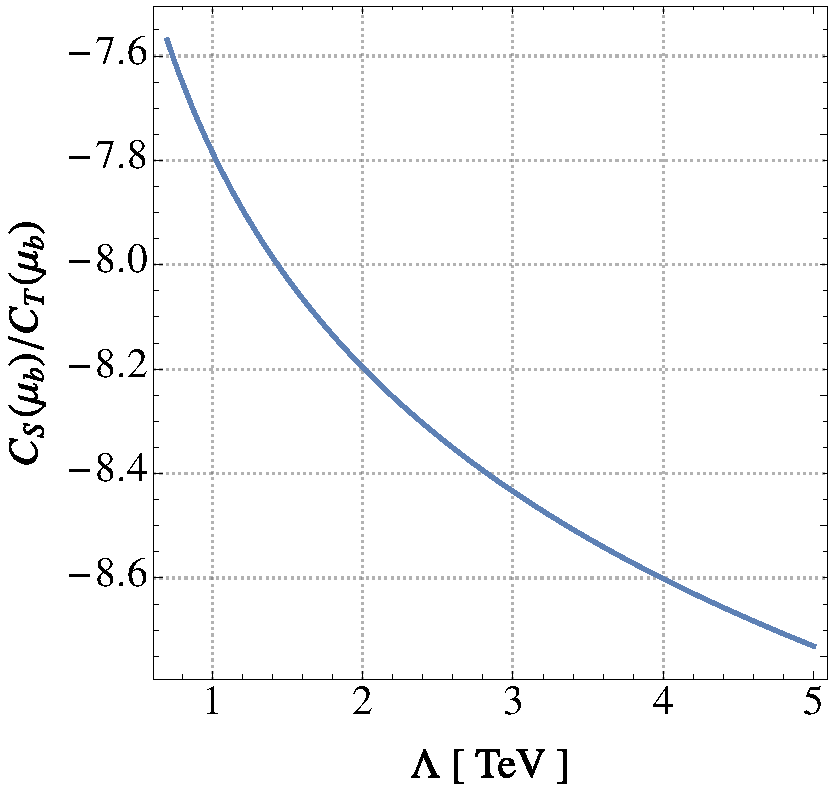
\includegraphics[width=0.6\linewidth]{runrat.pdf}
\caption[The dependence of the ratio of the tensor and scalar Wilson
coefficients evaluated at $\mu_b$ in $b \to c \ell \nu$ as a function of the
new-physics scale $\Lambda$, at which the ratio is $-4$.]{The dependence of the
  ratio of the tensor and scalar Wilson coefficients evaluated at $\mu_b$ in
  $b \to c \ell \nu$ as a function of the new-physics scale $\Lambda$, at which
  the ratio is $-4$. The figure depicts the values down to which the ratio
  $C_S/C_T$ evolves at $\mu_b$. For example, running from $\SI{1}{\TeV}$ to
  $\mu_b$ implies $C_S/C_T= -7.8$.}
\label{fig:ch3-runrat}
\end{figure}

We incorporate the new Belle combined measurement~\cite{Abdesselam:2019dgh} into
a fit of all measurements of $R_{D}$ and $R_{D^*}$ using the fitting software
\textsf{flavio}~\cite{Straub:2018kue}\footnote{We note that our fit does not
  include the measurements of $f_L^{D^*}$ and $R_{J/\psi}$, since errors here
  are still large. Instead, we take the central values from our fits and discuss
  predictions for these observables in
  section~\ref{sec:ch3-resultsanddiscussion}.}. The fit contours are shown in
Fig.~\ref{fig:ch3-fit}, with the fit excluding the new Belle measurement shown
with dashed contours to indicate its effect. We find the best-fit point
\begin{equation}
({C}_{V}, {C}_{S}) \approx (-0.18, 0.36),
\end{equation}
for the 2D fit to $\text{Re} C_{V}$ and
$\text{Re} C_{S} (\Lambda) = -4 C_T(\Lambda)$ at $\Lambda = \SI{2}{\TeV}$. We
also fit to $C_{V}$ with $C_{S}(\Lambda)=0$ and \textit{vice versa}. These
results are summarised in Table~\ref{tab:ch3-fitresults}. We comment here that
even for $S_{1}$ contributing to the direction
$C_{S}(\Lambda) = - 4 C_T(\Lambda)$, the vector operator will also always be
non-zero. This follows from the relation in Eq.~\eqref{eq:ch3-mixing}. The
leading contribution where only $x_{33}$ is non-zero is suppressed by
$|V_{ts}| \approx 0.04$, but this contribution can still be sizeable if $x_{33}$
is chosen to be large.

\begin{figure}
    \centering
    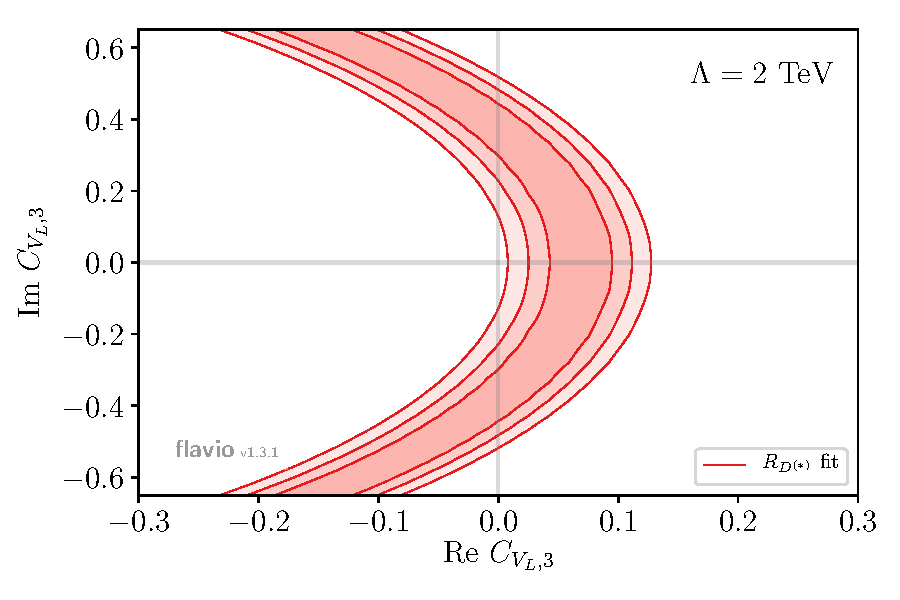
\includegraphics[width=0.62\linewidth]{rdrdstarfitCV}
    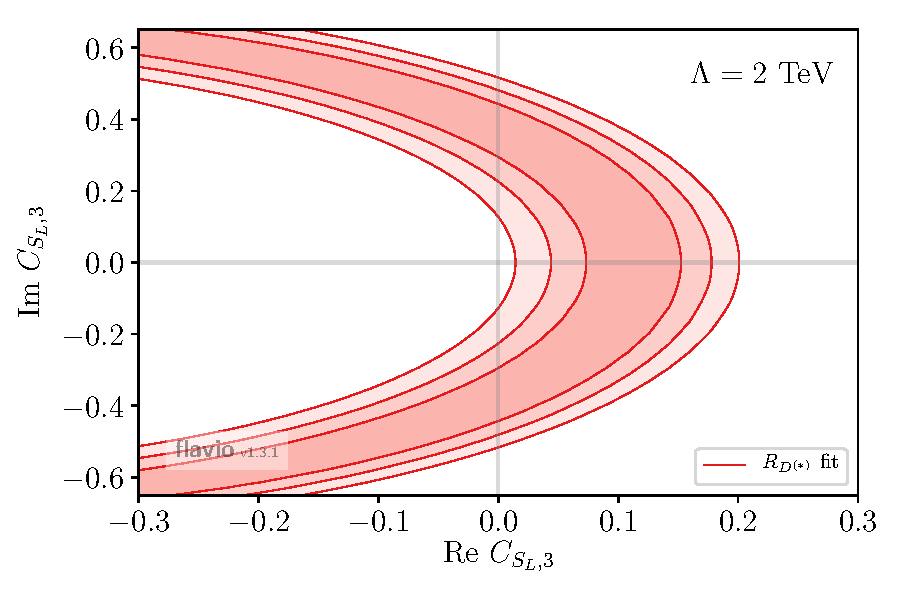
\includegraphics[width=0.62\linewidth]{rdrdstarfitCS}
    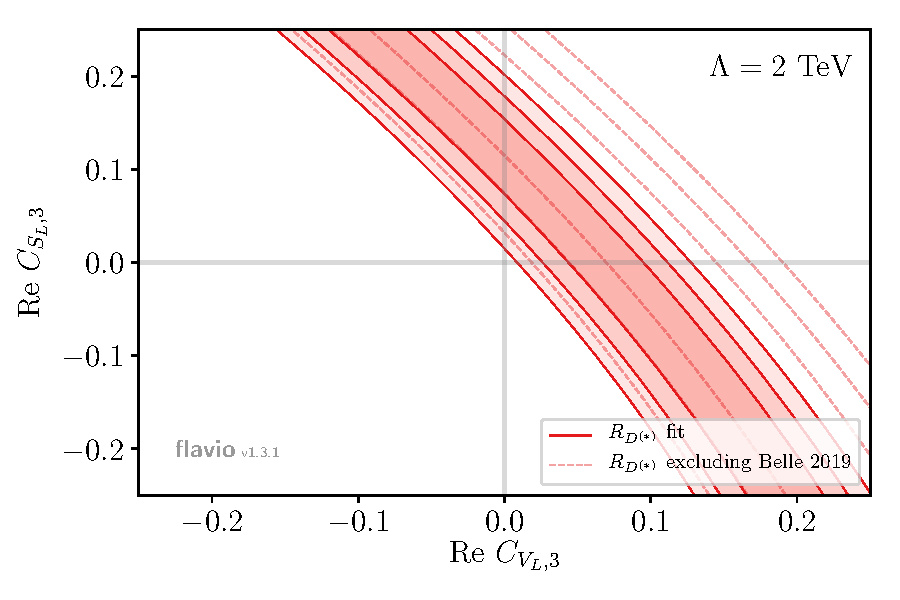
\includegraphics[width=0.62\linewidth]{rdrdstarfit}
    \caption[The results of our fit to $R_D$ and $R_{D^*}$ including the new
    Belle measurement~\cite{Abdesselam:2019dgh}.]{The results of our fit to
      $R_D$ and $R_{D^*}$ including the new Belle
      measurement~\cite{Abdesselam:2019dgh}. Contours show the $1$, $2$ and
      $3\sigma$ regions of the fit, dashed lines show the fit results without
      the recent Belle measurement. The scalar and tensor coefficients are run
      to the $b$-quark mass scale from $\SI{2}{\TeV}$. See
      Table~\ref{tab:ch3-fitresults} for central values and the text for more
      details.}
    \label{fig:ch3-fit}
\end{figure}

\begin{table}[t]
    \centering
    \begin{tabular}{c|ccc}
      \toprule
      Fit & Best fit & $1\sigma$ region & $2\sigma$ region \\
      \midrule
      $C_{V}$  & $0.069$ & $[0.044, 0.094]$ & $[0.026, 0.11]$ \\
      $C_{S}$ & $0.14$ & $[0.077, 0.15]$ & $[0.047, 0.18]$ \\
      $(C_{V}, C_{S})$ & $(-0.18, 0.36)$ & --- & --- \\
      \bottomrule
    \end{tabular}
    \caption[The results of our fit to $R_D$ and $R_{D^*}$ including the new
    Belle combined measurement~\cite{Abdesselam:2019dgh}.]{The results of our
      fit to $R_D$ and $R_{D^*}$ including the new Belle combined
      measurement~\cite{Abdesselam:2019dgh}. The first row shows the best fit
      point and $\sigma$-regions fitting to $C_{V}$ with all other operator
      coefficients vanishing. The second row shows the same for
      $C_{S}(\Lambda) = -4 C_T(\Lambda)$ for $\Lambda = \SI{2}{\TeV}$ and all
      other coefficients set to zero. The third row shows the best fit point for
      a 2D fit to $\text{Re}\, C_{V}$ and
      $\text{Re}\, C_{S}(\Lambda)= -4 \text{Re}\, C_T(\Lambda)$, again for
      $\Lambda = \SI{2}{\TeV}$.}
    \label{tab:ch3-fitresults}
\end{table}

\subsubsection{Neutral-current processes}
\label{sec:ch3-neutralcurrentprocesses}

The physics underlying the neutral-current $b \rightarrow s$ transitions in the
model can be described by the effective Lagrangian $\mathscr{L}_{\text{NC}}$:
\begin{equation}
  \mathscr{L}_{\text{NC}} = \frac{4 G_F}{\sqrt{2}} V_{tb} V^*_{ts} \frac{e^{2}}{16\pi^{2}} \sum_{IJ} C^\mu_{IJ}  \mathscr{O}^{\mu}_{IJ},
\end{equation}
where $I,J \in \{L, R\}$ and the operators in this chiral basis are defined
below in terms of $\mathscr{O}_{9,10}$. We note that this is equivalent to
Eq.~\eqref{eq:ch1-nc-lag}. Following the matching procedure performed in
Ref.~\cite{Misiak:1992bc}, we find that the field $S_{1}$ generates the
operators
\begin{equation}
  \label{eq:ch3-c9-c10-chiral}
  \begin{split}
  \mathscr{O}_{LL}^\mu \equiv
  \frac{1}{2}(\mathscr{O}_9^\mu - \mathscr{O}_{10}^\mu)
  &= (\bar{s}\gamma^\mu P_L b)(\bar{\mu} \gamma_\mu P_L \mu),\\
  \mathscr{O}_{LR}^\mu  \equiv
  \frac{1}{2}(\mathscr{O}_9^\mu + \mathscr{O}_{10}^\mu)
  &= (\bar{s}\gamma^\mu P_L
  b)(\bar{\mu}\gamma_\mu P_R \mu)
  \end{split}
\end{equation}
at the one-loop level with coefficients~\cite{Bauer:2015knc}
\begin{subequations} \label{eq:ch3-cllclreqs}
  \begin{align}
    C_{LL}^{S_{1},\mu} &= \frac{m_t^2}{8 \pi \alpha m_{S_{1}}^2}|z_{23}|^2 -
                         \frac{\sqrt{2}}{64\pi \alpha G_F m_{S_{1}}^2 V_{tb}V^*_{ts}}\sum_r x_{r 3}
                         x_{r 2}^* \sum_s |z_{2 s}|^2 , \label{eq:ch3-cll}\\
    \begin{split}
      C_{LR}^{S_{1},\mu} &= \frac{m_t^2}{16 \pi \alpha m_{S_{1}}^2}|y_{2 3}|^2
      \left[ \ln \frac{m_{S_{1}}^2}{m_t^2} - f \left( \frac{m_t^2}{m_W^2} \right)
      \right]\\ &\quad - \frac{\sqrt{2}}{64\pi \alpha G_F m_{S_{1}}^2
        V_{tb}V^*_{ts}}\sum_r x_{r 3} x_{r 2}^* \sum_s |y_{2 s}|^2, \label{eq:ch3-clr}
    \end{split}
  \end{align}
\end{subequations}
where
\begin{equation}
  f(x) = 1 - \frac{3}{x - 1} + \frac{3}{(x - 1)^2} \ln x.
\end{equation}
For the rest of the discussion we remove the $\mu$ superscript from the Wilson
coefficients and operators associated with $b \to s \mu \mu$, since we only
consider new-physics effects in the muonic mode. The dominant contributions are
from the box diagrams shown in Fig.~\ref{fig:ch3-boxes}. There are additional lepton
flavour universal contributions from $\gamma$ and $Z$ penguins, however these are
subdominant: the $Z$ penguins are suppressed by small neutrino masses and only
the small short-range contribution from the $\gamma$ penguins contributes to
$C^{S_{1}}_9$.

\begin{figure}[t]%
  \centering
  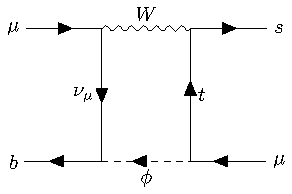
\includegraphics{boxes.pdf}
  \qquad
  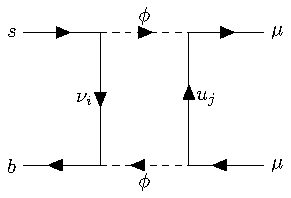
\includegraphics{boxes2.pdf}
  \caption{The box diagrams contributing to $C_{LL}^{S_{1}}$ and $C_{LR}^{S_{1}}$ in
    this scalar leptoquark model.}
  \label{fig:ch3-boxes}
\end{figure}

The authors of Refs.~\cite{Aebischer:2019mlg} conduct a global fit of all
available experimental data on the $b \rightarrow s$ decays. They find a good
fit to the data for the chiral coefficients generated by the leptoquark for
\begin{equation} \label{eq:ch3-cll12clr0}
  C_{LL}^{\text{NP}} \approx -1.0 \ \text{ and } \ C_{IJ}^{\text{NP}} \approx 0 \ \text{ otherwise},
\end{equation}
where new physics is assumed to significantly alter only the muonic mode and the
fit is performed for $C_{IJ} \in \mathbb{R}$. This choice of coefficients
results in a significantly improved fit to all of the $b \to s$ data, with a
total $6.6\sigma$ pull from the SM. Although a better fit to all of the data can
be achieved for $C_{LR}^{\text{NP}} < 0$ (this is clear from
Fig.~\ref{fig:ch1-c9-c10-fit}), the choice $C_{LR}^{\text{NP}}\approx 0$ allows
slightly smaller values of $C_{LL}^{\text{NP}}$ to explain the $R_{K^{(*)}}$
anomalies. The $2\sigma$ region for the fit is
$-1.4 \lesssim C_{LL}^{S_{1}} \lesssim -0.74$ with $C_{LR}^{S_{1}} = 0$. The
condition $C_{LR}^{S_{1}} \approx 0$ implies a suppression of the Yukawa
couplings $y_{2r}$, while $C_{LL}^{S_{1}} \approx -1$ requires large leptoquark
couplings to the second and third generation of left-handed quarks for the
second term in Eq.~\eqref{eq:ch3-cll}---corresponding to the second diagram in
Fig.~\ref{fig:ch3-boxes}---to dominate over the first, since it alone can be
negative.

\subsubsection{Anomalous magnetic moment of the muon}
\label{sec:ch3-gminus2}

The leptoquark also mediates one-loop corrections to the $\gamma \mu \mu$ vertex,
contributing to the muon anomalous magnetic moment. In the limit that $m_{S_{1}}^2
\gg m_t^2$, the contribution of $S_{1}$ to $a_\mu = (g - 2)_\mu/2$ is given
by~\cite{Bauer:2015knc, Djouadi:1989md, Chakraverty:2001yg, Cheung:2001ip}
\begin{equation} \label{eq:ch3-amu}
  a_\mu^{S_{1}} = \sum_{i} \frac{m_\mu m_{u_i}}{4\pi^2 m_{S_{1}}^2} \left(
    \frac{7}{4} - \ln \frac{m_{S_{1}}^2}{m_{u_i}^2} \right) \text{Re}
  (y_{2r} z_{2 i}) - \frac{m_\mu^2}{32 \pi^2 m_{S_{1}}^2}
  \left[ \sum_i |z_{2 i}|^2 + \sum_i |y_{2 i}|^2 \right],
\end{equation}
and the same-chirality terms are suppressed relative to the mixed-chirality term
by a factor of the muon mass, leading to the requirement of non-vanishing
right-handed couplings for an adequate explanation. We require that the
leptoquark contribution account for the measured anomaly, and thus that
$a_\mu^{S_{1}} = (287 \pm 80) \cdot 10^{-11}$~\cite{Davier:2010nc}.

The top-mass enhancement in the first term makes this the dominant contribution
in this model, and we illustrate the interesting values of $y_{32}$ and $z_{32}$
in Fig.~\ref{fig:ch3-gm2plots} for leptoquark mass values of
$m_{S_{1}}=\SI{1}{\TeV}$ and $m_{S_{1}}=\SI{5}{\TeV}$. Large $z_{23}$ values
assist the model's explanation of the $b \to s$ anomalies, hence a combined
explanation of this and the $(g-2)_\mu$ anomaly prefers a small $y_{23}$.
Explicitly, the condition~\cite{Bauer:2015knc}
\begin{equation} \label{eq:ch3-bnamueq}
  -20.7 (1 + 1.06 \ln\hat{m}_{S_{1}}) \text{Re}(y_{23} z_{23}) \approx 0.08 \hat{m}_{S_{1}}^2
\end{equation}
must be satisfied to meet the central value of the measurements of $a_\mu$ in
this minimal case.

\begin{figure}[t]
  \centering
\begin{minipage}[t]{.45\linewidth}
\centering 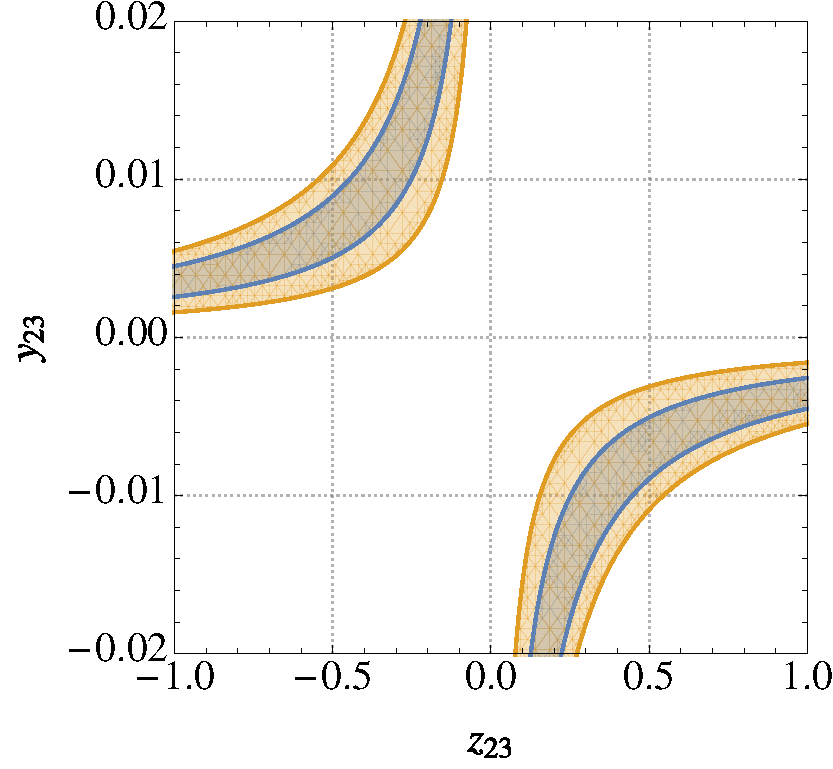
\includegraphics[scale=0.47]{gm2plot.pdf}
\phantomsubcaption \label{fig:ch3-gm2plot}
\end{minipage}%
\hfill
\begin{minipage}[t]{.45\linewidth}
\centering 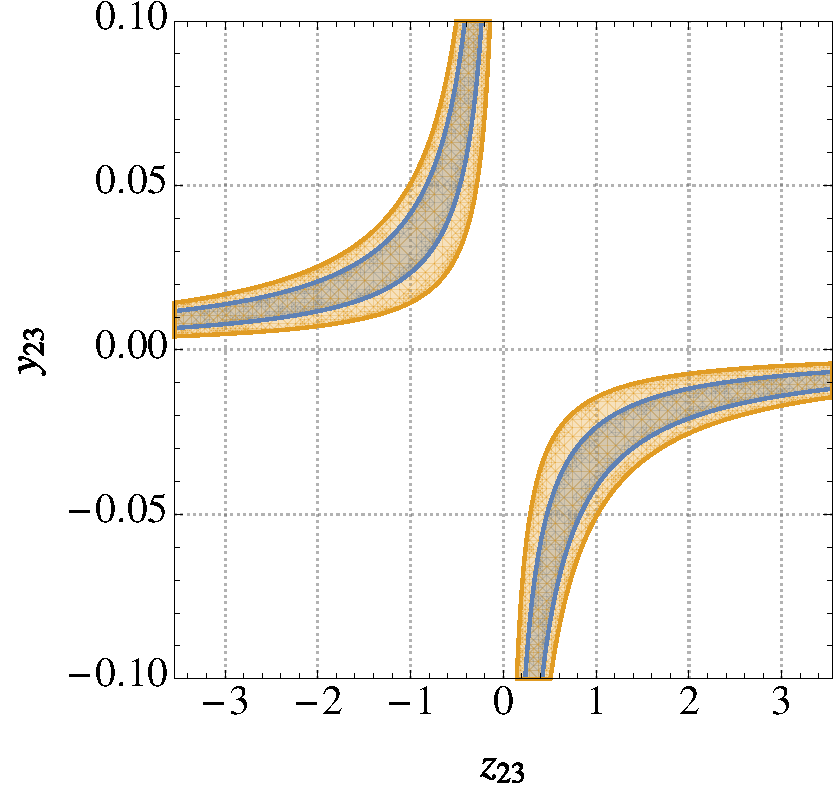
\includegraphics[scale=0.455]{gm2plot2.pdf}
\phantomsubcaption \label{fig:ch3-gm2plot2}
\end{minipage}
\caption[The $1$ and $2\sigma$ allowed regions for $a_\mu$ in the
$y_{23}$--$z_{23}$ plane for leptoquark masses of $m_{S_{1}} = \SI{1}{\TeV}$
(left) and $m_{S_{1}} = \SI{5}{\TeV}$ (right).]{The $1$ and $2\sigma$ allowed
  regions for $a_\mu$ in the $y_{23}$--$z_{23}$ plane for leptoquark masses of
  $m_{S_{1}} = \SI{1}{\TeV}$ (left) and $m_{S_{1}} = \SI{5}{\TeV}$ (right). The
  top-mass enhancement in the first term of Eq.~\eqref{eq:ch3-amu} allows the model
  to accommodate $a_\mu$ with very small values for $|y_{23}|$ with
  $z_{23} \neq 0$.}\label{fig:ch3-gm2plots}
\end{figure}

\subsection{Constraints}
\label{sec:ch3-constraints}

We proceed by studying the constraints important for the leptoquark $S_{1}$ in
the regions of parameter space dictated by the flavour anomalies. This analysis
includes the constraints imposed by $B$, $K$ and $D$ meson decays,
$B_s$--$\bar{B}_s$ mixing, lepton-flavour violating processes and electroweak
measurements.

Many of these processes are studied in the context of an effective-operator
framework. Since much of the nomenclature for four-fermion operator coefficients
is often only based on the Lorentz-structure of each term, keeping the naming
conventions present in the flavour-physics literature for each process can lead
to ambiguity. For this reason we index each effective Lagrangian appearing in
this section and retain the common names for each term, with the Lagrangian's
index prepended to the label. For example, $C_{i,V_L}$ might correspond to the
coefficient of an operator like $(\bar{S_{1}} \gamma_\mu P_L \chi)(\bar{\psi}
\gamma^\mu P_L \omega)$ in $\mathscr{L}_i$, where $S_{1},\chi,\psi,\omega$
represent Fermion fields. For clarity we remind the reader that the coefficients
of $\mathscr{L}_{\textsc{CC}}$ and $\mathscr{L}_{\textsc{NC}}$ from the previous
section are left unindexed.

For the reader's convenience, we signpost the important results
of this section below.

\paragraph{Constraints on the left-handed couplings.} A feature of the BN model
is that the effective operators mediating the $b \to s \mu \mu$ decays are
generated through box diagrams, since $S_{1}$ only couples down-type quarks to
neutrinos at tree-level. As a consequence, the large Yukawa couplings required
to meet the $b \to s$ measurements will mediate FCNC processes with a neutrino
pair in the final state---processes to which they are related by
$\textrm{SU}(2)_L$ invariance---at tree level. This makes the $b \to s \nu \nu$
decays and $K^+ \to \pi^+ \nu \nu$ very constraining for this model's
explanation of the $b \to s$ anomalies. The former decay is more important,
since it involves the combination of left-handed couplings present in
Eq.~\eqref{eq:ch3-cllclreqs}: $\sum_{r} x_{r3}x^*_{r2}$, and essential to ensure
a negative value for $C^{S_{1}}_{LL}$. The leptoquark also contributes to
$B_s$--$\bar{B}_s$ mixing through box diagrams similar to those given in
Fig.~\ref{fig:ch3-boxes} with neutrinos running through both internal fermion
lines. We find measurements of $B_s$--$\bar{B}_s$ mixing to be more constraining
than those of FCNC decays for leptoquark masses larger than a few \TeV. For
small leptoquark masses, precision electroweak measurements of the
$Z\ell \bar{\ell}$ couplings place upper bounds on the sum of the absolute
squares of left-handed couplings, and a relative sign difference between
couplings to the third-generation quarks and those to the second implies the
possibility of a mild cancellation taming these effects. A very important
constraint on the left-handed coupling $|x_{22}|$ can be derived from the meson
decay $D^0 \to \mu \mu$, a large value of which aids the explanation of
$R_{K^{(*)}}$ in this scenario. It has also recently been pointed
out~\cite{Becirevic:2016oho} that the LFU evident in the ratio
$R_{D}^{\mu/e} = \Gamma(B\rightarrow D \mu \nu) / \Gamma(B\rightarrow D e \nu)$
represents a significant hurdle to the leptoquark's explanation of the $b \to s$
data, and we discuss this constraint below.

Constraints on the product of left-handed couplings discussed above also
frustrate the model's attempts to explain measurements of the ratios $R_D$ and
$R_{D^{*}}$, specifically in those areas of parameter space suggested by
new-physics effects only in $C_V^{rs}$. This implies the need for non-vanishing
right-handed couplings $y_{rs}$ so that the $C_{S} = - 4 C_{T}$ direction is
generated.

\paragraph{Constraints on the right-handed couplings.} The right-handed
couplings $y_{rs}$ are generally less constrained in this leptoquark model,
since they mediate interactions involving fewer fermion species. The most
stringent limits come from mixed-chirality contributions to tau decays such as
$\tau \to \mu \mu \mu$ and $\tau \to \mu \gamma$, as well as the precision
electroweak measurements mentioned above. Many right-handed couplings also
feature in the model's contributions to $B$, $D$, and $K$ decays.

\subsubsection{Semileptonic charged-current processes}
\label{sec:ch3-semileptonicchargedcurrentprocesses}

Leptonic and semileptonic charged-current processes are a sensitive probe of the
model we study, since the leptoquark $S_{1}$ provides tree-level channels for
leptonic pseudoscalar meson decays and semileptonic decays of the tau. In order
to describe these processes, we generalise the Lagrangian presented in
Eq.~\eqref{eq:ch3-CCHam} to
\begin{equation} \label{eq:ch3-CCHam2}
  \begin{split}
    \mathscr{L}^{rstu}_{1} &= -\frac{4 G_F}{\sqrt{2}} V_{u_r d_s} \left[
      C_{1,V}^{rstu}(\bar{u}_r \gamma^\mu P_L d_s)(\bar{e}_t \gamma_\mu P_L
      \nu_{u}) + C^{rstu}_{1,S} (\bar{u}_r P_L d_s)(\bar{e}_t P_L\nu_{u}) \right. \\
    &\quad \left. + C^{rstu}_{1,T} (\bar{u}_r \sigma^{\mu \nu} P_L d_s)
      (\bar{e}_t \sigma_{\mu \nu} P_L \nu_{u})\right],
  \end{split}
\end{equation}
where the vector, scalar and tensor Wilson coefficients at the leptoquark mass
scale now read
\begin{subequations} \label{eq:ch3-ccoperators2}
  \begin{align}
    C_{1,V}^{rstu} &= \frac{1}{2 \sqrt{2} G_F V_{u_r d_s}} \frac{z_{ts}^* x_{ur}}{2m_{S_{1}}^2} + \delta_{tu},\\
    C_{1,S}^{rstu} &= \frac{1}{2 \sqrt{2} G_F V_{u_r d_s}} \frac{y_{t s} x_{u r}}{2m_{S_{1}}^2},\\
    C_{1,T}^{rstu} &= -\frac{1}{4} C_{1,S}^{rstu}, \label{eq:ch3-ccops3}
  \end{align}
\end{subequations}
in analogy with Eqs.~\eqref{eq:ch3-ccoperators}. The leptonic decay rate for a
pseudoscalar meson $P_{rs} \sim \bar{u}_r d_s$ is then given
by~\cite{Becirevic:2016oho}
\begin{equation} \label{eq:ch3-plnu}
  \begin{split}
    \Gamma(P_{rs} \to e_t \nu_{u}) &= \frac{G_F^2 m_P |V_{u_r d_s}|^2}{8\pi} f_P^2 m_{e_t}^2 \left( 1 - \frac{m_{e_u}^2}{m_P^2} \right)^2\\ &\quad \cdot \left| C_{1,V}^{rstu} - C_{1,S}^{rstu} \frac{m_P^2}{m_{e_t}(m_{u_r} + m_{d_s})} \right|^2,
  \end{split}
\end{equation}
where $f_P$ is the pseudoscalar meson decay constant. As before, we account for
the effect of the running of $\alpha_s$ from the high scale to the scales
appropriate for each decay for the scalar operator. We take the relevant scale
to be $\mu = \overline{m_c} = \SI{1.27}{\GeV}$ for the $D$ meson decays and
$\mu = \SI{2}{\GeV} $ for the $K$ decays, since this is the matching scale used
in Ref.~\cite{Aoki:2016frl}, from which we take the decay constants. Explicitly,
\begin{equation}
  C_{1,S} (\mu) = \left[\frac{\alpha_s(m_b)}{\alpha_s(\mu)} \right]^{\frac{\gamma_S}{2\beta_0^{(4)}}} \left[\frac{\alpha_s(m_t)}{\alpha_s(m_b)} \right]^{\frac{\gamma_S}{2\beta_0^{(5)}}} \left[\frac{\alpha_s(\Lambda)}{\alpha_s(m_t)} \right]^{\frac{\gamma_S}{2\beta_0^{(6)}}} C_{1,S}(\Lambda),
\end{equation}
while the running for the scalar operator featuring in the $B$ decays is the
same as in Eq.~\eqref{eq:ch3-runningrd}. Eq.~\eqref{eq:ch3-plnu} is finely sensitive to
the Wilson coefficient $C_{1,S}$ since it has the effect of lifting the chiral
suppression of the SM due to the charged lepton mass in the denominator of the
last term. Recent work~\cite{Becirevic:2016oho} has pointed out the importance
of considering the decays $B \to \ell \bar{\nu}$, $K \to \ell \bar{\nu}$, $D_s
\to \ell \bar{\nu}$ and $B \to D^{(*)} \ell \nu$, to which we also add a
discussion of $\tau \to K \nu$ and $B_c \to \ell \bar{\nu}$ below. In addition,
for each relevant process we calculate a LFU ratio, since in many cases these
are well measured quantities which constitute powerful probes of any new-physics
attempting to explain $R_{D^{(*)}}$ or $R_{K^{(*)}}$. We summarise the limits
and values we take for these decays and their relevant ratios in
Table~\ref{tbl:ch3-decays}. All values of the decay constants used throughout this
discussion are taken from Ref.~\cite{Aoki:2016frl}.

\begin{table}[t]
  \centering
  \begin{tabular}{cc}
    \toprule
    Observable & Experimental value \\
    \midrule
    $\text{Br}(K\to\mu\nu)$       & $(63.56 \pm 0.11) \%$  \\
    $\text{Br}(D_s \to \mu \nu)$  & $(0.549 \pm 0.016) \%$ \\
    $\text{Br}(D_s \to \tau \nu)$ & $(5.55 \pm 0.24) \%$   \\
    $\text{Br}(B \to \mu \nu)$    & $(6.46 \pm 2.22 \pm 1.60) \cdot 10^{-7}$~\cite{Sibidanov:2017vph}  \\
    $\text{Br}(B \to \tau \nu)$   & $(1.09 \pm 0.24) \cdot 10^{-4}$ \\
    $\text{Br}(B_c \to \tau \nu)$   & $\lesssim 30 \%$~\cite{Alonso:2016oyd} \\
    \arrayrulecolor{black!30}\midrule
    $r_K^{e/\mu} = \frac{\Gamma(K \to e\nu)}{\Gamma(K\to \mu\nu)}$ & $(2.488 \pm 0.009) \cdot 10^{-5}$\\
    $R_{K}^{\tau/\mu} = \frac{\Gamma(\tau \to K\nu)}{\Gamma(K\to \mu\nu)}$ & $(1.101 \pm 0.016) \cdot 10^{-2}$\\
    $R_{D_s}^{\tau/\mu} = \frac{\Gamma(D_s \to \tau\nu)}{\Gamma(D_s\to \mu\nu)}$ & $10.73 \pm 0.69^{+0.56}_{-0.53}$~\cite{Zupanc:2013byn}\\
    % $R^{\mu/e}_{K\to\pi} = \frac{\Gamma(K \to \pi \mu \nu)}{\Gamma(K \to \pi e \nu)}$ & $0.6608 \pm 0.0029$\\
    $R_D^{\mu/e} = \frac{\Gamma(B \to D \mu \nu)}{\Gamma(B \to D e \nu)}$ & $0.995 \pm 0.022 \pm
0.039$~\cite{Glattauer:2015teq}\\
    $R_{D^*}^{e/\mu} = \frac{\Gamma(B \to D^* e \nu)}{\Gamma(B \to D^* \mu \nu)}$ & $1.04 \pm 0.05 \pm 0.01$~\cite{Abdesselam:2017kjf}\\
    \arrayrulecolor{black!100}\bottomrule
  \end{tabular}
  \caption[A table summarising the experimental values we take for the various
  leptonic branching ratios and LFU ratios considered in this section.]{A table
    summarising the experimental values we take for the various leptonic
    branching ratios and LFU ratios considered in this section. Measurements
    quoted without explicit citation are taken from Ref.~\cite{Olive:2016xmw}.}
    \label{tbl:ch3-decays}
\end{table}

The ratio
\begin{equation} \label{eq:ch3-rkemu}
  r_K^{e/\mu} = \frac{\Gamma(K \to e \nu)}{\Gamma(K \to \mu \nu)}
\end{equation}
is one of the most precisely measured quantities in weak hadronic physics. As
such, the consideration of next-to-leading-order corrections becomes important
for our phenomenological analysis of the effects of the leptoquark $S_{1}$ on
these decays. Electroweak effects contributing to $r_K^{e/\mu}$ have been
calculated to order $e^2p^4$ in chiral perturbation theory,
e.g.~\cite{Cirigliano:2007ga, Finkemeier:1994ev}. Higher order contributions to
the quotient Eq.~\eqref{eq:ch3-rkemu} are proportional to the lowest order
contribution: $r_K^{e/\mu, (0)}$, calculated directly from Eq.~\eqref{eq:ch3-plnu}.
Including the effects of leading higher-order logarithms through $\Delta_{LL}$,
Eq.~\eqref{eq:ch3-rkemu} can be written
\begin{equation}
  r_K^{e/\mu} = r_K^{e/\mu, (0)} \left( 1 + \Delta^K_{e^2 p^2} + \Delta^K_{e^2 p^4} + \cdots \right) \left( 1 + \Delta_{LL} \right)
\end{equation}
and we take $\Delta_{LL} = 0.055 \%$, $\Delta_{e^2 p^2}^K = -3.786 \%$ and
$\Delta_{e^2 p^4}^K = (0.135 \pm 0.011) \%$~\cite{Cirigliano:2007ga} in our
calculation.

One can extend the study of lepton-flavour universality in leptonic kaon decays
by considering the crossed process $\tau \to K \nu$. More specifically, the
ratio
\begin{equation}
  R_K^{\tau/\mu} = \frac{\Gamma(\tau \to K\nu)}{\Gamma(K \to \mu \nu)}
\end{equation}
can be used to derive constraints on the muon and tau couplings of the
leptoquark $S_{1}$, and a similar approach has been taken to constrain the
couplings of a vector leptoquark in Ref.~\cite{Fajfer:2015ycq}. For the
numerator, we find
\begin{equation}
  \Gamma(\tau \to K \nu) = \frac{G_F^2 |V_{us}|^2}{8 \pi} f_K^2 m_\tau^3 \left( 1 - \frac{m_K^2}{m_\tau^2} \right)^2 \sum_{r} \left| C_{1,V}^{123r}  - C_{1,S}^{123r} \frac{m_K^2}{m_\tau(m_u + m_s)} \right|^2,
\end{equation}
and the ratio $R_K^{\tau/\mu}$ is required to lie within $2\sigma$ of its
experimental value: $(1.101 \pm 0.016) \cdot 10^{-2}$~\cite{Olive:2016xmw}.

Pion leptonic decays have been well-studied in the context of leptoquark models,
and measurements of the ratio $R_\pi^{\mu/e} = \Gamma(\pi \to \mu
\nu)/\Gamma(\pi \to e \nu)$ demand that leptoquark interactions with the
electron and first-generation quarks are small\footnote{In the most minimal
  case, a non-zero $x_{2 1}$ implies $z_{2 1} \approx x_{2 1}$ and these
  couplings alone are sufficient to mediate the decay $\pi^+ \rightarrow \mu^+
  \nu$.}~\cite{Buchmuller:1986iq, Davidson:1993qk}. The electron and down-quark
couplings play no role in the anomalies we consider in this work, and we only
require that the appropriate couplings are small enough to evade these
constraints.

\paragraph{Comments on lepton flavour universality in $B \to
  D^{(*)} (e,\mu) \nu$.} An additional constraint comes from the
observation that LFU is respected in the ratio of decay rates
\begin{equation}
  R_{D^{(*)}}^{\mu/e} = \frac{\Gamma(B \rightarrow
    D^{(*)} \mu \nu)}{\Gamma(B \rightarrow
    D^{(*)} e \nu)},
\end{equation}
implying a tension with the purported violation in $\mu$--$e$ universality
evident in $R_{K^{(*)}}$. This constraint has been studied in
Ref.~\cite{Becirevic:2016oho}, where it was concluded that the leptoquark model
cannot respect this constraint while explaining the suppression of $R_K$ in the
absence of the right-handed couplings $y_{rs}$. The ratio has been measured to
be $R_D^{\mu/e} = 0.995 \pm 0.022 \pm 0.039$~\cite{Glattauer:2015teq}, while the
reciprocal is presented for the $D^*$ ratio:
$R_{D^{*}}^{e/\mu} = 1.04 \pm 0.05 \pm 0.01$~\cite{Abdesselam:2017kjf}. In the
case of $R_D^{\mu/e}$, $2\sigma$ consistency with the measurement allows for an
approximately $10\%$ deviation from the SM prediction, a weaker bound than that
presented in Ref.~\cite{Becirevic:2016oho}, while the recent Belle result for
$R_{D^{*}}^{e/\mu}$ permits only a $4\%$ deviation for contributions to the
muonic mode. We find that these constraints become less important for leptoquark
masses larger than $\SI{1}{\TeV}$, permitting sizeable contributions to $C_{LL}$
in this model. We illustrate this point in the top plot of
Fig.~\ref{fig:ch3-LFUratios}, where random points passing all of the constraints
presented in our analysis except $R_{D^{*}}^{e/\mu}$ are presented in the
$C_{LL}$--$R_{D^{*}}^{\mu/e}$ plane. The parameters and ranges taken in our scan
are the same as those of scan I in Sec.~\ref{sec:ch3-resultsanddiscussion} in
which masses are sampled randomly from the range $[1,5]~\TeV$. The complementary
set-up for $R_{D}^{e/\mu}$ is shown in the bottom figure of
Fig.~\ref{fig:ch3-LFUratios}, \textit{mutatis mutandis}.

\begin{figure}
  \centering
  \begin{minipage}[t]{0.6\linewidth}
    \centering 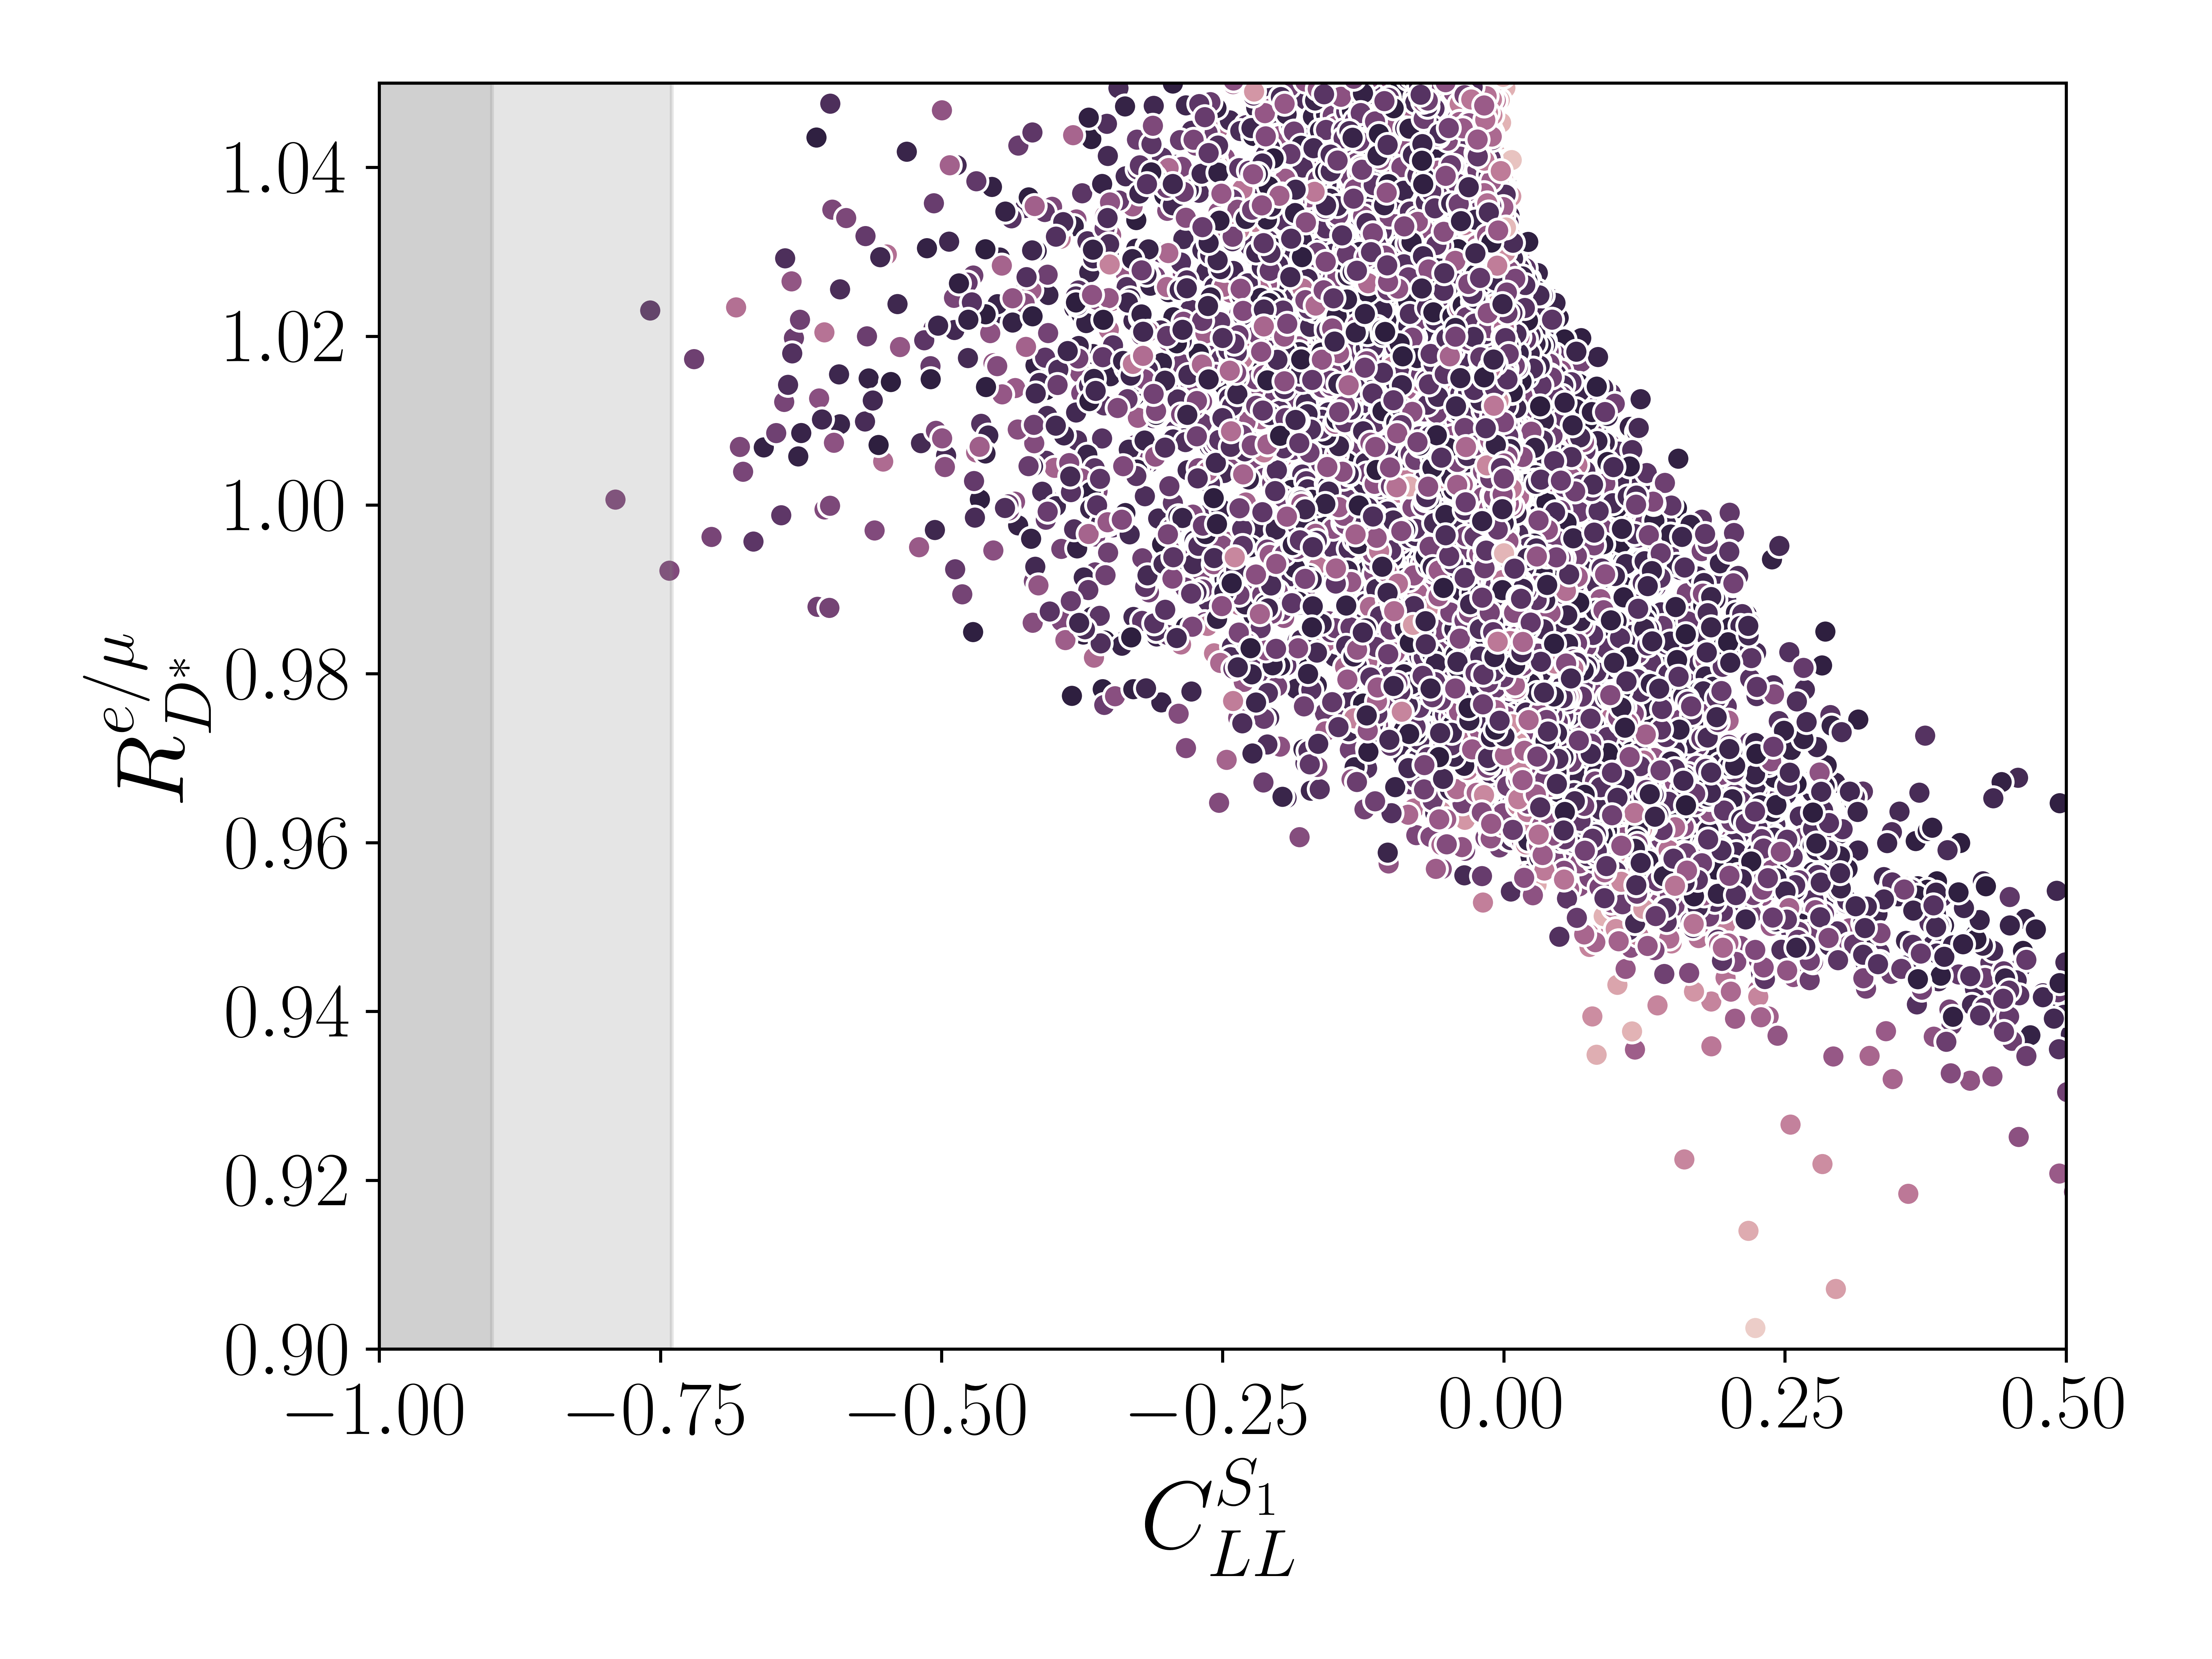
\includegraphics[width=\linewidth]{new_becTestStar.png}
  \end{minipage}
  \hfill
  \begin{minipage}[t]{0.6\linewidth}
    \centering 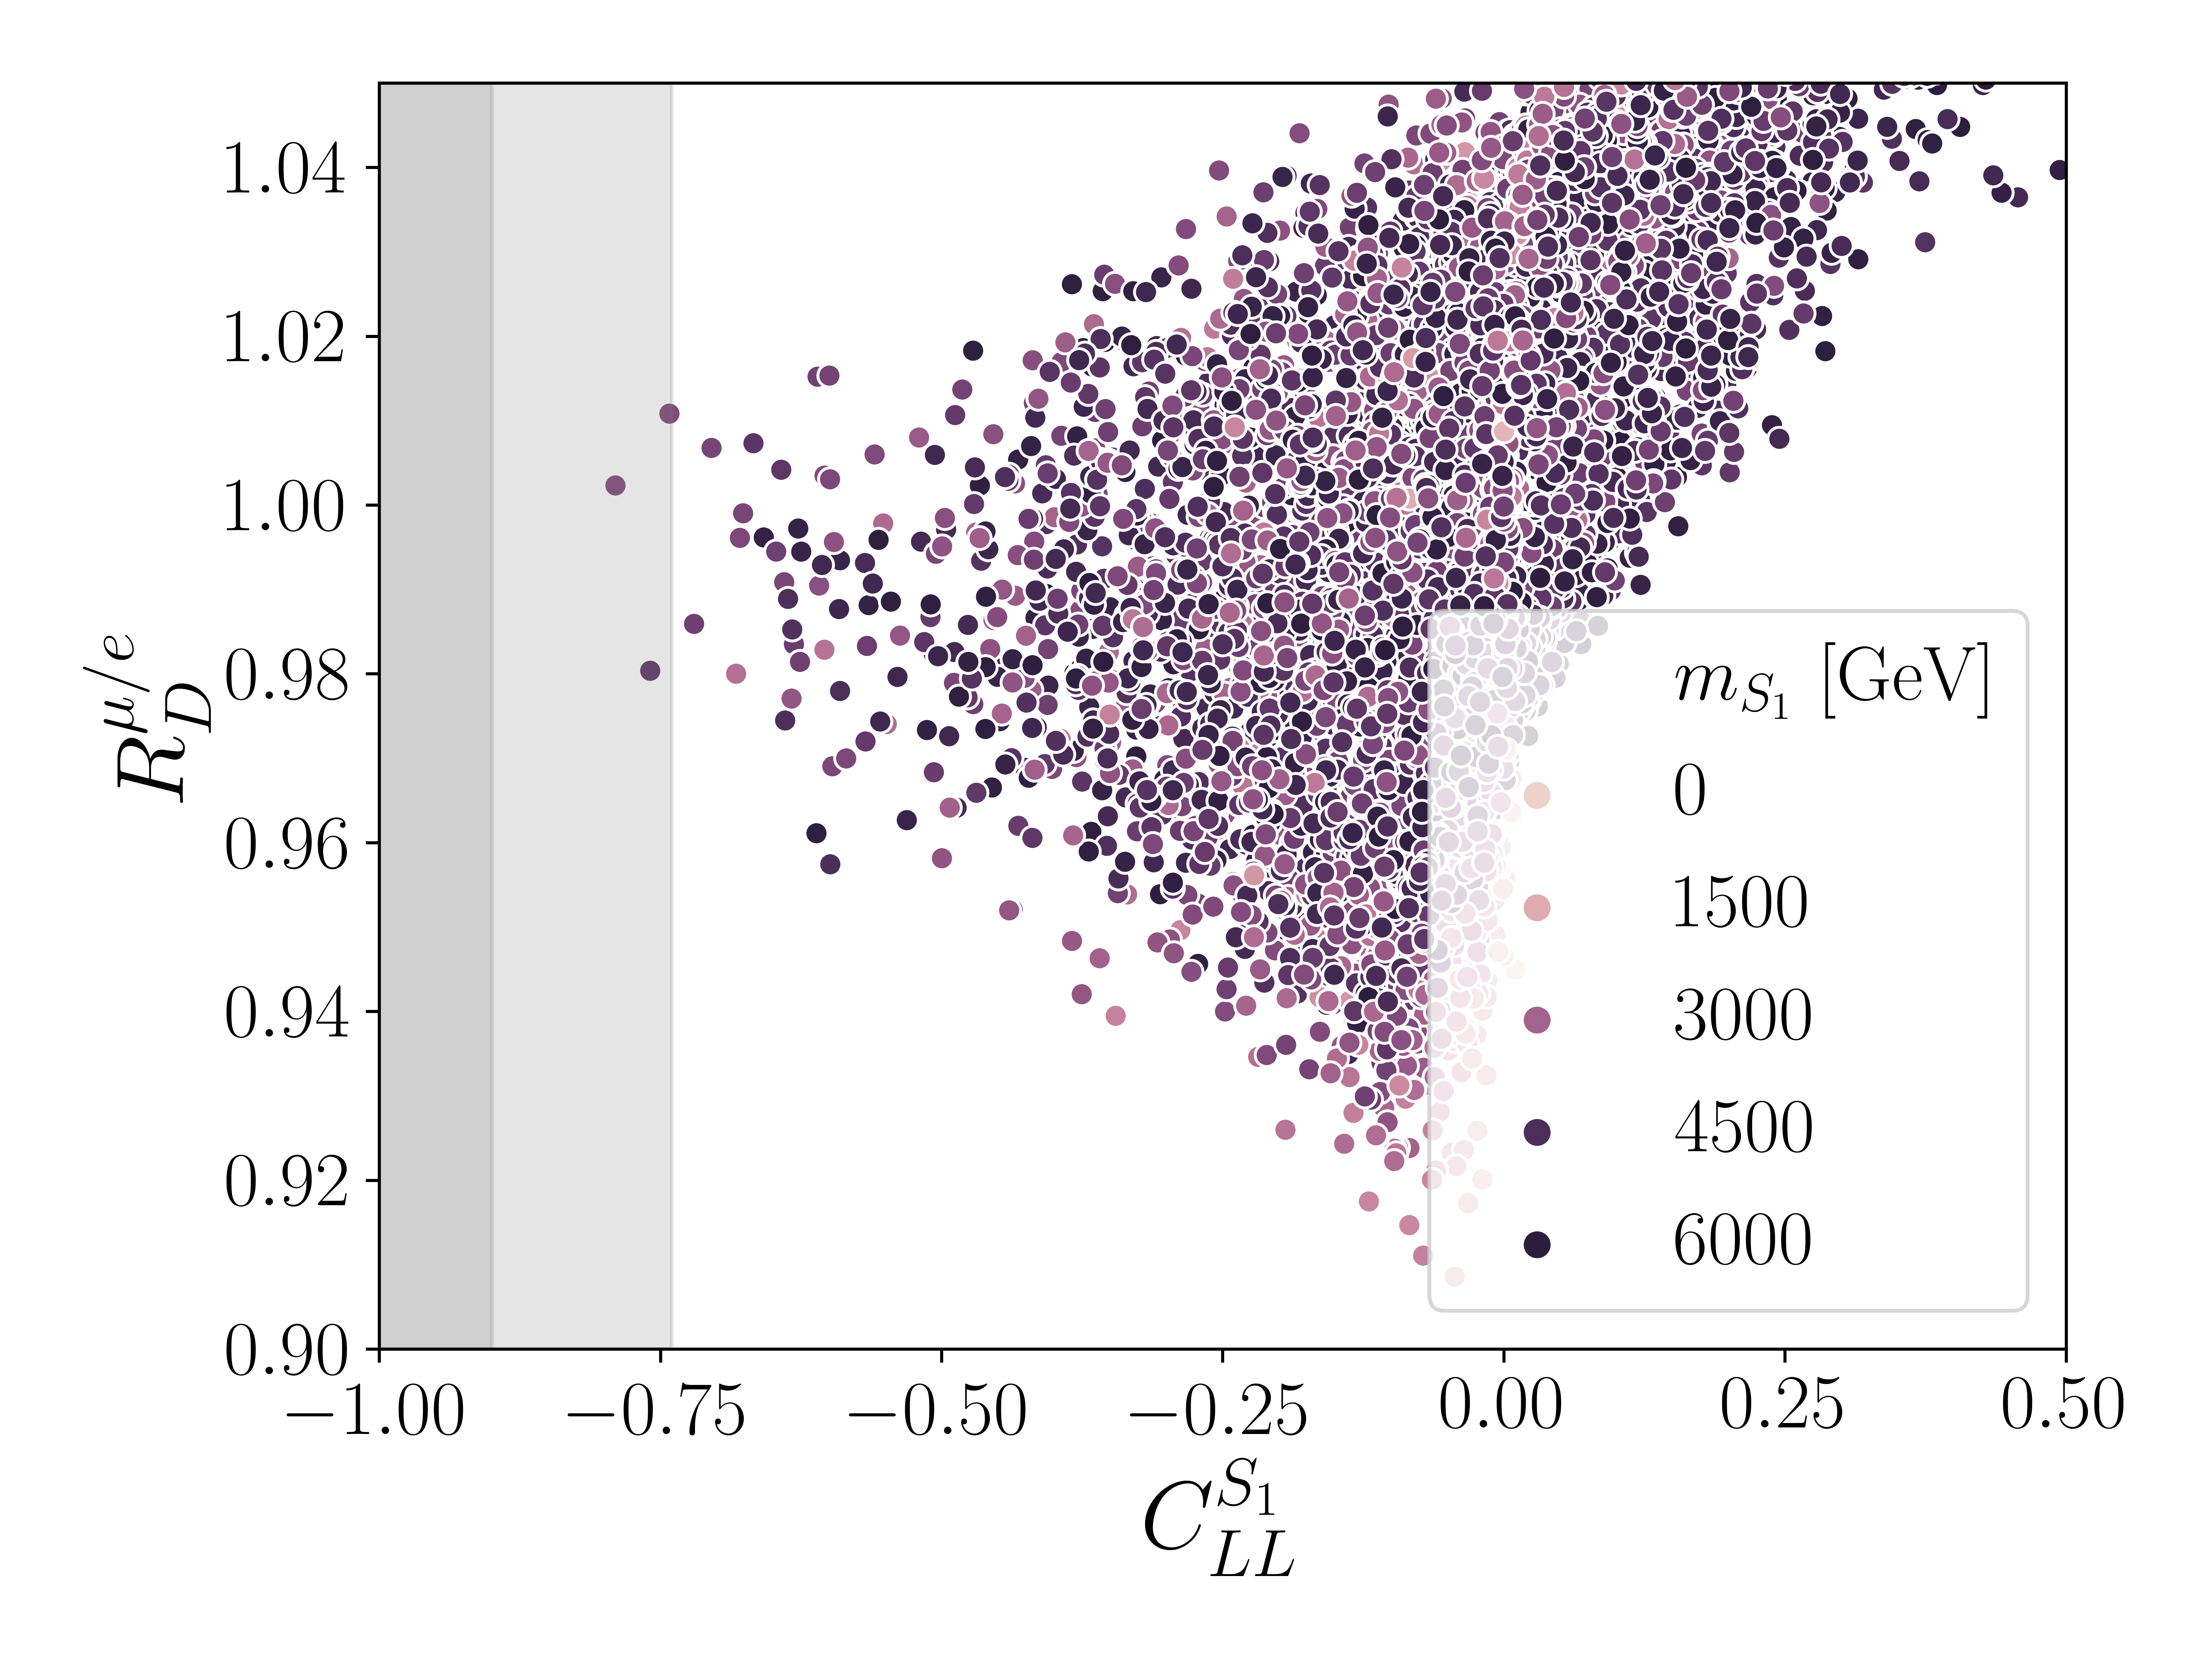
\includegraphics[width=\linewidth]{new_becTest.png}
  \end{minipage}
  \caption[The results of our random scan showing $C_{LL}$ against $R_D^{\mu/e}$
  (bottom) and $R^{e/\mu}_{D^*}$ (top) for the parameter choices detailed in
  Sec.~\ref{sec:ch3-resultsanddiscussion} for `scan I', in which the leptoquark
  mass is allowed to vary to values as large as \SI{5}{\TeV}.]{The results of
    our random scan showing $C_{LL}$ against $R_D^{\mu/e}$ (bottom) and
    $R^{e/\mu}_{D^*}$ (top) for the parameter choices detailed in
    Sec.~\ref{sec:ch3-resultsanddiscussion} for `scan I', in which the
    leptoquark mass is allowed to vary to values as large as \SI{5}{\TeV}. For
    leptoquark masses between 3 and \SI{5}{\TeV}, the tension in the $b \to s$
    data can be significantly resolved while keeping LFU effects between
    electron and muon $b \to c$ modes mild.}
  \label{fig:ch3-LFUratios}
\end{figure}

\paragraph{Comments on $B_c \to \tau \nu$.} The leptonic decays of the charmed
$B$ meson have not yet been measured---few $B_c$ mesons are produced at $e^+e^-$
$B$-factories and the leptonic mode cannot be reliably reconstructed at
LHC\textit{b}. Despite this, measurements of the $B_c$ lifetime have recently
been shown to imply serious constraints~\cite{Li:2016vvp, Alonso:2016oyd} for
models explaining $R_{D^{(*)}}$ with contributions to the operator $C_S^{3r}$
defined in Eq.~\eqref{eq:ch3-CCHam}. Here, we wish to point out that the $B_c \to
\tau \nu$ rate remains SM-like in this leptoquark model due to the presence of
the tensor contribution $C_T^{3r}$, and thus that measurements of the $B_c$
lifetime do not constitute a serious constraint on the model.

In Fig.~\ref{fig:ch3-bctaunu1} we plot the branching ratio
$\text{Br}(B_c \to \tau \nu)$ in this leptoquark model against interesting
values of $R_{D^*}$, in the spirit of Fig.~1 of Ref.~\cite{Alonso:2016oyd}. The
blue curve represents the contribution from only the Wilson coefficient $C_S$,
while the orange curve represents the contribution from the scalar leptoquark
$S_{1}$ where the scalar and tensor contributions are related through
Eq.~\eqref{eq:ch3-ccops3}. The presence of both the scalar and tensor
contributions results renders the branching ratio sufficiently small in the
region of interest.

\begin{figure}[t]
  \centering 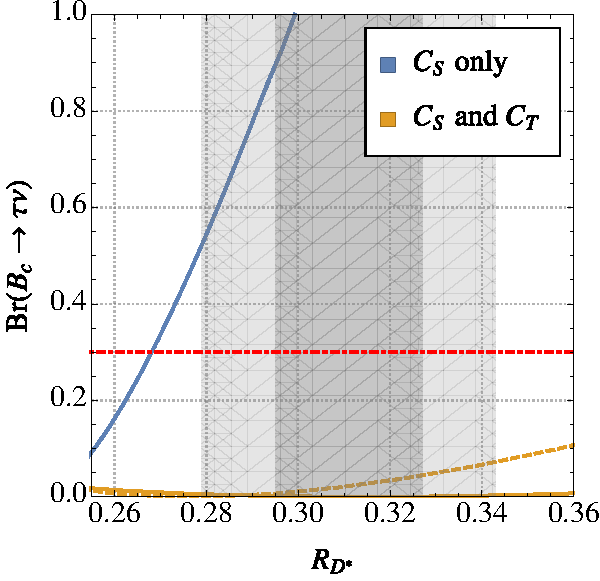
\includegraphics[scale=0.75]{bctaunu.pdf}
  \caption[The branching ratio $\text{Br}(B_c \to \tau \nu)$ against $R_{D^*}$
  with new physics only in $C_S$ (solid blue) and new physics in both $C_S$ and
  $C_T$ satisfying $C_S / C_T = -4$ (solid orange) and $C_S / C_T = -7.8$
  (dashed orange).]{The branching ratio $\text{Br}(B_c \to \tau \nu)$ against
    $R_{D^*}$ with new physics only in $C_S$ (solid blue) and new physics in
    both $C_S$ and $C_T$ satisfying $C_S / C_T = -4$ (solid orange) and
    $C_S / C_T = -7.8$ (dashed orange). The $30\%$ limit is shown in red
    (dot-dashed). The dark and light grey regions represent the $1$ and
    $2\sigma$ regions for $R_{D^{(*)}}$. In this leptoquark model,
    $\text{Br}(B_c\to \tau \nu)$ remains $\lesssim 30\%$ in the region of
    interest.}
  \label{fig:ch3-bctaunu1}
\end{figure}

\subsubsection{Lepton flavour violating processes}
\label{sec:ch3-leptonflavourviolatingprocesses}

The lepton-flavour symmetries present in the SM are broken by the
Yukawa couplings of the leptoquark to the SM fermions. This implies that $S_{1}$
can mediate processes that do not conserve lepton flavour, of which those
considered in our analysis are $e_i \to e_j \gamma$, $e_i \to e_j
e_k e_l$ and muon--electron conversion in nuclei: $\mu \ce{^{A}_{Z}N} \to
e \ce{^{A}_{Z}N}$. We use the expressions for these processes found in the
Appendix of Ref.~\cite{Angel:2013hla}, adapted to the case of one leptoquark,
and direct the reader there for more details. We impose the following limits for
the constraints:
\begin{align}
  \text{Br}(\tau \to \mu \gamma) &< 4.4 \cdot 10^{-8}~\text{\cite{Aubert:2009ag}},\\
  \text{Br}(\tau \to \mu \mu \mu) &< 2.1 \cdot 10^{-8}~\text{\cite{Miyazaki:2011xe}},\\
  \text{Br}(\mu \ce{^{197}_{79}Au} \to e \ce{^{197}_{79}Au}) &< 7.0 \cdot 10^{-13}~\text{\cite{Bertl:2006up}}.
\end{align}
In the $\mu \to e$ transition, we only consider muon--electron conversion since
this is the most stringent of the muon's lepton-flavour-violating (LFV) decay
modes that the leptoquark can mediate~\cite{Angel:2013hla, Babu:2010vp,
  Cai:2014kra}. The tree-level contributions to muon--electron conversion imply
very strong constraints on the coupling combinations involved. Assuming no
accidental cancellation between terms, the order-of-magnitude
bounds~\cite{Angel:2013hla}
\begin{align}
  z_{21}y_{11}^*, y_{21}z_{11}^* &\lesssim [4 \cdot 10^{-9}, 7 \cdot 10^{-8}] \frac{m_{S_{1}}^2}{m_W^2},\\
  z_{21}z_{11}^*, y_{21}y_{11}^* &\lesssim [10^{-8}, 10^{-7}] \frac{m_{S_{1}}^2}{m_W^2}.
\end{align}
can be evaded with small electron couplings.

\subsubsection{Rare meson decays}
\label{sec:ch3-raremesondecays}

The most important rare meson decays remain to be mentioned. We group them here
and separate their discussion based on the species of lepton in the final state.
The decays studied are: (1) $B \to K \nu \nu$ and $K^+ \to \pi^+ \nu \nu$,
involving neutrinos, and (2) $D^0 \to \mu \mu$ and $D^+ \to \pi^+ \mu \mu$,
involving charged leptons.

The decays $B \rightarrow K^{(*)} \nu \nu$ and $K^+ \rightarrow \pi^+ \nu \nu$ heavily
constrain the combination of Yukawa couplings $x_{rs}$ in this model since the
SM contributions proceed at loop-level, while our leptoquark mediates such
neutral-current quark decays at tree-level. The physics describing this class of
decays is described by the effective Lagrangian~\cite{Altmannshofer:2009ma,
  Buras:2004uu}
\begin{equation}
  \begin{split}
    \mathscr{L}_2^{rstu}
    &= \frac{8 G_F}{\sqrt{2}} \frac{e^2}{16 \pi^2} V_{t d_r} V^*_{t d_s} \left[ C^{rstu}_{2,L} (\bar{d}_r \gamma_\mu P_{L} d_s)(\bar{\nu}_t
      \gamma^\mu P_L \nu_u) \right. \\ &\quad \left. + C^{rstu}_{2,R} (\bar{d}_r \gamma_\mu P_{R} d_s)(\bar{\nu}_t
      \gamma^\mu P_L \nu_u) \right] + \text{ h.c.}
  \end{split}
\end{equation}
and operator coefficients
\begin{equation}
  C_{2,L}^{rstu} = -\frac{\sqrt{2}\pi^2}{e^2 G_F m_{S_{1}}^2}\frac{x^*_{t s} x_{u r}}{V_{t d_r}V_{t d_s}^*} + C_L^{\text{SM}}\delta_{tu}, \quad C_{2,R}^{rstu} = 0,
\end{equation}
where $C_L^{\text{SM}} = -X(m_t^2/m_W^2)/s_w^2$. The SM loop function $X(x)$ is
given by~\cite{Buras:2004uu, Altmannshofer:2009ma, Buchalla:1998ba,
  Misiak:1999yg}
\begin{equation}
  X(x) = \frac{x}{8} \left[ \frac{x+2}{x-1} + \frac{3x-6}{(x-1)^2} \ln x \right],
\end{equation}
and the ratios
$R_{K^{(*)}}^{\nu\nu} \equiv \Gamma(B\rightarrow K^{(*)} \nu \nu)/\Gamma(B\rightarrow K \nu \nu)_{\text{SM}}$
are constrained to satisfy $R_K^{\nu\nu} < 3.9$ and $R_{K^{*}}^{\nu\nu} < 2.7$
at $90\%$ C.L.~\cite{Grygier:2017tzo}. We find
\begin{equation} \label{eq:ch3-rknunu}
  \begin{split}
    R_{K^{(*)}}^{\nu\nu} &= \frac{1}{3}\sum_{rs}\frac{|C_{2,L}^{32rs} |^2 }{|C_L^{\text{SM}}|^2}\\
    &= 1 + \frac{a^2}{3m_{S_{1}}^4}\sum_{rs}\left|\frac{x^*_{r 2} x_{s 3}}{V_{tb}
        V^*_{ts}}\right|^2 - \frac{2a}{3m_{S_{1}}^2} \sum_r \text{Re} \left(\frac{x^*_{r
        2} x_{r 3}}{V_{tb} V^*_{ts}}\right),
  \end{split}
\end{equation}
where $a = \sqrt{2} \pi^2 / (e^2 G_F |C_L^{\text{SM}}|)$. Due to the absence of
right-handed currents, our model predicts $R_K^{\nu\nu} = R_{K^{*}}^{\nu\nu}$
although the bound on $R_{K}^{\nu\nu}$ is slightly weaker, as is that for
the inclusive decay. A conservative limit on the combination
$(\sum x^*_{r 2} x_{r 3})/\hat{m}^2_{S_{1}}$ can be derived using the Schwartz
inequality~\cite{Bauer:2015knc}:
\begin{equation} \label{eq:ch3-bnunucond}
  -0.05 \lesssim \frac{[\mathbf{x}^\dagger \mathbf{x}]_{23}}{\hat{m}^2_{S_{1}}} \lesssim 0.1,
\end{equation}
where we have assumed $\text{Arg}(x_{r2}^*x_{r3}) = \text{Arg}(V_{tb}V_{ts}^*)$.
We emphasise that this bound represents an insufficient condition for the model
to respect the experimental limits. In Fig.~\ref{fig:ch3-rknunuallowed} we present
the allowed region for non-zero $x_{32}$ and $x_{33}$ and $m_{S_{1}} = \SI{1}{\TeV}$---a coupling texture interesting for explaining $R_{D^{(*)}}$, although
heavily constrained by $R_{K^{*}}^{\nu\nu}$.

\begin{figure}[t]
  \centering 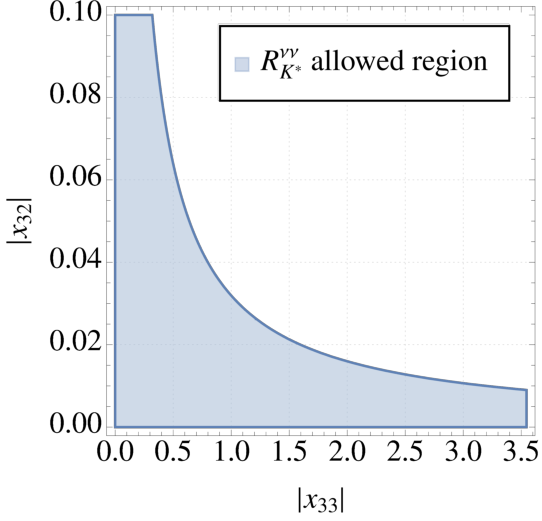
\includegraphics[scale=0.85]{rknunuallowed.pdf}
  \caption[The region allowed by experimental limits on the decay
  $B \to K^{*} \nu \nu$ in the $|x_{33}|$--$|x_{32}|$ plane for $m_{S_{1}} = \SI{1}{\TeV}$.]{The region allowed by experimental limits on the decay
    $B \to K \nu \nu$ in the $|x_{33}|$--$|x_{32}|$ plane for $m_{S_{1}} = \SI{1}{\TeV}$. All other couplings are switched off. A large value of $|x_{33}|$
    is essential to explaining $R_{D^{(*)}}$, and the figure implies that such a
    requirement keeps $|x_{32}|$ small.}
  \label{fig:ch3-rknunuallowed}
\end{figure}

The decay $K^+ \rightarrow \pi^+ \nu \nu$ constitutes the most stringent
constraint on our model from the kaon sector~\cite{Kumar:2016omp}. We
find
\begin{equation}
  \begin{split}
  \text{Br}(K^+\rightarrow \pi^+ \nu \nu) &= \frac{1}{3}\sum_{rs} \kappa_+ \left[ \left(\text{Im} \frac{ V_{ts}V_{td}^* s_w^2 C_{2,L}^{21rs} }{\lambda^5} \right)^2  \right. \\ &\quad \left. +  \left( \text{Re} \frac{ V_{tb}V_{ts}^* s_w^2 C_{2,L}^{21rs}}{\lambda^5} + P_{(u,c)} \delta_{rs} \right)^2 \right],
  \end{split}
\end{equation}
by adapting Eq.~(3.29) of Ref.~\cite{Altmannshofer:2009ma}, where the
factor $\kappa_+ = (5.27 \pm 0.03) \cdot 10^{-11}$ is due mainly to hadronic
matrix elements, $\lambda$ is the CKM Wolfenstein parameter, $P_{(u,c)} = 0.41
\pm 0.05$ accounts for the effects of light-quark loops, and the small
electromagnetic corrections have been neglected. The branching ratio for the
decay has most recently been measured by the E949 collaboration to be
$\text{Br}(K^+ \rightarrow \pi^+ \nu \nu) = (1.73^{+1.15}_{-1.05}) \cdot
10^{-10}$~\cite{Artamonov:2009sz}. A conservative limit can be placed on the
combination of new-physics couplings featuring in $C_{2,L}^{21rs}$ by
considering only same-flavoured neutrinos in the final state of the decay. Under
the assumptions that the couplings involved are real and that only one
combination dominates, we find
\begin{equation} \label{eq:ch3-kpinunubound}
  -9.1 \cdot 10^{-4} < \frac{[\mathbf{x}^\dagger \mathbf{x}]_{21}}{\hat{m}_{S_{1}}^2} < 4.8 \cdot 10^{-4}.
\end{equation}
This bound can be avoided by considering a suppression of the leptoquark
couplings to the first generation of quarks.

In this leptoquark model, the coupling of the $c$-quark to the charged leptons
is essential for the explanation of the $b \to c \tau \nu$ anomalies. Also, as
discussed earlier, the up-quark couplings cannot be entirely avoided due to the
stringency of Eq.~\eqref{eq:ch3-kpinunubound} and the mixing of
Eq.~\eqref{eq:ch3-mixing}. These factors make the physics of operators of the form
$\mathscr{O}_{rstu} \sim (u_r \Gamma u_s) (e_t \Gamma e_u)$ an important
source of constraint on this model. Additionally, in order to ensure
$C_{LL}^{S_{1}} \approx -1.2$ in the model's original conception, an ansatz for
$z_{rs}$ was chosen such that $|z_{22}|$ takes $\mathscr{O}(1)$ values.
Constraints from the decays $D^0 \rightarrow \mu \mu$ and $D^+ \rightarrow \pi^+
\mu \mu$ are especially worrying in this case, since the leptoquark mediates
these processes at tree-level. Even within the context of vanishing
first-generation couplings, one cannot avoid inducing new-physics interactions
involving up quarks because of the mixing of Eq.~\eqref{eq:ch3-mixing}. The
new-physics contributions to decays of the form $u_r \to u_s e_t e_u$ can
be contained within the effective Lagrangian
\begin{equation}
  \label{eq:ch3-charm-lag}
  \begin{split}
    \mathscr{L}_3^{rstu}
    &= \frac{4 G_F}{\sqrt{2}} \bigg[  C^{rstu}_{3, V_{R}}  (\bar{u}_r \gamma_\mu P_R u_s)(\bar{e}_t \gamma^\mu P_R e_u) + C_{3, V_{L}}^{rstu} (\bar{u}_r \gamma_\mu P_L u_s)(\bar{e}_t \gamma^\mu P_L e_u)\\ &\quad + C_{3, T}^{rstu} (\bar{u}_r \sigma_{\mu\nu} P_R u_s)(\bar{e}_t \sigma^{\mu\nu} P_R e_u) + C_{3, S_L}^{rstu} (\bar{u}_r P_L u_s)(\bar{e}_t P_L e_u)\\ &\quad + C_{3, S_R}^{rstu}(\bar{u}_r P_R u_s)(\bar{e}_t P_R e_u) + \text{h.c.}
    \bigg],
  \end{split}
\end{equation}
with coefficients $C_{3,r}$ at the leptoquark mass scale given by
\begin{align}
  C_{3,\{V_L,V_R\}}^{rstu} &= \frac{1}{2\sqrt{2} G_F} \left\{ \begin{matrix} z_{ts}z_{lr}^*\\ y^*_{ts} y_{ur} \end{matrix}  \right\} \frac{1}{2 m_{S_{1}}^2},\\
  C_{3,\{S_L,S_R\}}^{rstu} &= \frac{1}{2\sqrt{2} G_F} \left\{ \begin{matrix} z_{ts}y_{ur}\\ y^*_{ts} z^*_{ur} \end{matrix}  \right\} \frac{1}{2 m_{S_{1}}^2},\\
  C_{3,T}^{rstu} &= -\frac{1}{4} C^{rstu}_{3,S_L}.
\end{align}
For the scalar and tensor operators we account for the running of $\alpha_s$
down to the charm-quark mass scale as in
Sec.~\ref{sec:ch3-semileptonicchargedcurrentprocesses}.

For the leptonic decay, we find
\begin{subequations} \label{eq:ch3-Dmumu}
  \begin{align}
    \begin{split}
      \Gamma(D^0 \rightarrow \mu \mu) &= \frac{f_D^2 m_D^3 G_F^2}{32\pi}\left(\frac{m_D}{m_c}\right)^2\beta_\mu
      \Bigg[ \left| C_{3,S_L}^{2122}-C_{3,S_R}^{2122}\right|^2 \beta_\mu^2  \\
      & \quad + \left| C_{3,S_L}^{2122}+ C_{3,S_R}^{2122} -\frac{2 m_\mu m_c}{m_D^2} (C_{3,V_L}^{2122}+C_{3,V_R}^{2122})\right|^2 \Bigg] \end{split} \\
    \begin{split}
      &= \frac{f_D^2 m_D^3}{512 \pi m_{S_{1}}^4}
      \left( \frac{m_D}{m_c} \right)^2 \beta_\mu \left[ \vphantom{\frac{2 m_\mu
            m_c}{m_D^2}} | y^*_{22} z_{2 1}^* - z_{2 2} y_{2 1} |^2
        \beta_\mu^2 \eta^2 \right. \\
      &\quad \left. + \left| \eta(y_{2 2}^* z_{2 1}^* +
          z_{2 2} y_{2 1}) - \frac{2 m_\mu m_c}{m_D^2} (z_{2 2} z_{2 1}^*
          + y_{2 2}^* y_{2 1}) \right|^2 \right] \; ,
    \end{split}
  \end{align}
\end{subequations}
where $\beta_\mu = (1 - 4m_\mu^2/m_D^2)^{1/2} \approx 0.99$,
$f_D = \SI{212(2)}{\MeV}$~\cite{Aoki:2016frl} and
$\eta = C_{3,S_{L}}^{2122}(\overline{m_c}) / C_{3,S_{L}}^{2122}(m_{S_{1}})$. In
the limit that the left-handed contribution dominates, the bound
\begin{equation} \label{eq:ch3-zmc}
  |x_{2 2}| < 0.46 \hat{m}_{S_{1}}
\end{equation}
can be derived from the experimental upper limit $\text{Br}(D^0 \rightarrow
\mu\mu) < 7.6 \cdot 10^{-9}$~\cite{Aaij:2013cza} assuming $x_{23} \ll x_{22}$.
One can arrange for a mild cancellation between the same- and mixed-chirality
terms in Eq.~\eqref{eq:ch3-Dmumu} by allowing the right-handed couplings $y_{2
  (1,2)}$ to take $\mathscr{O}(0.1)$ values, however this creates tensions with
other meson decays such as $D_s \rightarrow \mu \nu$, $K \rightarrow \mu \nu$
and $D^+ \rightarrow \pi^+ \mu \mu$, and we find no overlapping allowed region.

For the decay $D^+ \to \pi^+ \mu \mu$, we implement the calculation of
Ref.~\cite{Fajfer:2015mia}. The branching ratio
\begin{equation}
  \text{Br}(D^+ \to \pi^+ \mu^+ \mu^-) < 8.3 \cdot 10^{-8},
\end{equation}
is measured by extrapolating spectra over the resonant
region~\cite{Aaij:2013sua}, while the bounds on the separate high- and low-$q^2$
bins are
\begin{align}
  \text{Br}(D^+ \to \pi^+ \mu^+ \mu^-)_{q^2 \in [1.56, 4.00]}   &< 2.9 \cdot 10^{-8},\label{eq:ch3-Dpimumu1}\\
  \text{Br}(D^+ \to \pi^+ \mu^+ \mu^-)_{q^2 \in [0.0625, 0.276]} &< 2.5 \cdot 10^{-8},\label{eq:ch3-Dpimumu2}
\end{align}
where $q^2$ ranges are given in $\GeV^{2}$. Both Eq.~\eqref{eq:ch3-Dpimumu1} and
Eq.~\eqref{eq:ch3-Dpimumu2} are imposed in our numerical scans.

\subsubsection{Meson mixing}

A complementary constraint on the left-handed couplings can be derived from
$B_s$--$\bar{B}_s$ mixing, providing a stronger bound than $R_K^{\nu\nu}$ for
leptoquark masses larger than a few \TeV. The UT\textit{fit} collaboration
determines constraints on $\Delta F = 2$ processes in terms of the quotient of
the meson mixing amplitude and the SM prediction:
\begin{equation}
  C_{B_s} e^{2i \phi_{B_s}} \equiv \frac{\langle B_s | \mathscr{H}^{\Delta F = 2} | \bar{B}_s \rangle}{\langle B_s | \mathscr{H}^{\Delta F = 2}_{\text{SM}} | \bar{B}_s \rangle} \ ,
\end{equation}
and the current best fit values for these parameters are
$C_{B_s} = 1.110 \pm 0.090$ and
$\phi_{B_s} = (0.42 \pm 0.86)^\circ$~\cite{Bona:2007vi}. In the notation of
Ref.~\cite{Bona:2007vi}, our leptoquark only generates the effective operator
$Q^{rs}_1 = C^{bs}_1(\bar{q}_{ra} \gamma_\mu P_L q_s^a)(\bar{q}_{tb} \gamma^\mu P_L q_u^b)$
through box diagrams with neutrinos and leptoquarks in the loop. The relevant
operator coefficient, defined at the high scale $\Lambda$, is
\begin{equation} \label{eq:ch3-Q1}
  C^{bs, S_{1}}_{1}(\Lambda) = \frac{1}{128 \pi^2} \left(\sum_r \frac{x_{r 3}^* x_{r 2}}{m_{S_{1}}}\right)^2 \ ,
\end{equation}
in the limit of vanishing SM fermion masses. The SM processes involve similar
box diagrams with top quarks and $W$ bosons in the loop, inducing the Wilson
coefficient (see e.g.~\cite{Fleischer:2008uj})
\begin{equation}
  C^{bs, \text{SM}}_{1} = \frac{G_F^2 m_W^2}{4\pi^2}(V_{tb}^*V_{ts})^2 S_0(m_t^2 / m_W^2) \ ,
\end{equation}
where $S_0(x)$ is the well-known Inami-Lim function~\cite{Inami:1980fz}:
\begin{equation}
  S_0(x) = \frac{x^3 -11x^2 + 4x}{4(x-1)^2} - \frac{3x^3}{2(x-1)^3} \ln x \ .
\end{equation}
We account for the effect of the running of $\alpha_s$ down to $m_W$ for the
coefficient $C^{bs, S_{1}}_{1}$ to compare with the SM result
using~\cite{Aebischer:2017gaw}
\begin{equation}
  C_1^{bs, S_{1}}(m_W) =  \left[\frac{\alpha_s(m_t)}{\alpha_s(m_W)}\right]^{\frac{\gamma}{2\beta_0^{(5)}}} \left[\frac{\alpha_s(\Lambda)}{\alpha_s(m_t)}\right]^{\frac{\gamma}{2\beta_0^{(6)}}} C_1^{bs, S_{1}}(\Lambda) \ ,
\end{equation}
where $\gamma = 4$ and $\beta_0^{(n_f)} = 11 - 2 n _f / 3$. The combination of
left-handed couplings in Eq.~\eqref{eq:ch3-Q1} is thus required to satisfy
\begin{equation} \label{eq:ch3-BsBsbar}
  C_{B_s} e^{2i \phi_{B_s}} = 1 + \frac{1}{32 G_F^2 m_W^2 S_0(m_t^2/m_W^2)} \left(  \frac{\eta^\prime}{V_{tb}^* V_{ts}} \sum_r \frac{x_{r 3}^* x_{r 2}}{m_{S_{1}}} \right)^2 \ ,
\end{equation}
where $\eta^\prime = C_1^{bs, S_{1}}(m_W) / C_1^{bs, S_{1}}(m_{S_{1}})$.

\subsubsection{Precision electroweak measurements}

The Yukawa interactions of the leptoquark with both left- and right-handed SM
fermions give corrections to many electroweak observables. Precision
measurements of these have been translated into bounds on dimension-six
operators in the literature, and we proceed by applying the results of a recent
fit to the electroweak precision data~\cite{Ciuchini:2013pca}. Specifically, we
consider the way in which the couplings $x_{rs}$ and $y_{rs}$ are constrained by
precision electroweak measurements of the $Z \ell \bar{\ell}$ couplings $g_L$
and $g_R$. These receive corrections from leptoquark loops in our
model~\cite{Bauer:2015knc}:
\begin{equation} \label{eq:ch3-neccond}
  \begin{split}
  \delta g_X^{e_r} &= (-1)^{\delta_{XR}} \frac{3}{32 \pi^2} \frac{m_t^2}{m_{S_{1}}^2} \left( \ln \frac{m_{S_{1}}^2}{m_t^2} - 1 \right) |\lambda^X_{r 3}|^2 \\ &\quad - \frac{1}{32 \pi^2}\frac{m_Z^2}{m_{S_{1}}^2}\sum_{s}^2 |\lambda^X_{r s}|^2 \left[ \left( \delta_{XL} - \frac{4 s_w^2}{3} \right) \left( \ln\frac{m_{S_{1}}^2}{m_Z^2} + i\pi + \frac{1}{3} \right) - \frac{s_w^2}{9}\right],
  \end{split}
\end{equation}
where $X \in \{L,R\}$, $\lambda^L_{rs} = z_{rs}$ and $\lambda^R_{rs} = y_{rs}$.
From Eq.~(3.28) and Table 10 of Ref.~\cite{Ciuchini:2013pca}, we calculate the
conservative constraints
\begin{equation} \label{eq:ch3-eqZll}
  \text{Re}\delta g_L^{e_r} \in [-8.5, 12.0] \cdot 10^{-4}, \quad \text{Re}\delta g_R^{e_r} \in [-5.4, 6.7] \cdot 10^{-4}
\end{equation}
at $95\%$ confidence from the fit results obtained using the large-$m_t$
expansion. The expressions in Eq.~\eqref{eq:ch3-eqZll} are conservative since we do
not account for correlations between different operators but this does not
affect our results in an important way. The results of the fit are sensitive to
the interference between the SM and leptoquark contributions, hence only the
real part of the $\delta g_I^{e_r}$ is constrained.

\section{Results and discussion}
\label{sec:ch3-resultsanddiscussion}

Below we study the extent to which the experimental anomalies in $R_{D^{(*)}}$,
the $b \to s$ transition and $(g-2)_\mu$ can be accommodated in light of the
constraints presented in Sec.~\ref{sec:ch3-constraints}. We first consider each
anomaly separately and then present the combined parameter space.

For all of the random scans in this section our Monte Carlo strategy proceeds as
follows. We sample random real values of the free parameters $x_{rs}$ for
$r,s \neq 1$ and leptoquark masses in the range $\hat{m}_{S_{1}} \in [0.6, 5]$.
Values are sampled from the region described in Eq.~\eqref{eq:ch3-bnunucond}---a
necessary condition for the $x_{rs}$ to respect the bound from $B \to K\nu\nu$,
discussed in Sec.~\ref{sec:ch3-raremesondecays}---and the perturbativity bound
$|x_{rs}| \leq \sqrt{4\pi}$ is imposed at sampling. The values chosen for the
right-handed couplings $y_{rs}$ depend on the process studied, although we find
that only the $y_{2r}$ and $y_{32}$ are important for our analysis. Two scans
are performed, here labelled I and II. Scan I explores the parameter space
associated with the $b \to s$ anomalies and thus only contains the couplings
featuring in Eq.~\eqref{eq:ch3-cllclreqs}, while scan II is intended to
elucidate the parameter space associated with both the neutral-current and
charged-current anomalies, hence $y_{32}$ is included. An important difference
between scans I and II is that the former allows $C_{LR}^{S_{1}} \neq 0$,
although this comes at the expense of fewer points passing all of the
constraints since the couplings $y_{22}$ and $y_{23}$ are heavily constrained by
semileptonic charged-current processes discussed in
Sec.~\ref{sec:ch3-semileptonicchargedcurrentprocesses}. Explicitly, the
parameters and respective ranges over which they are scanned are as follows.
\begin{description}
\item [Scan I.] $6 \cdot 10^6$ points sampled from the region in
  Eq.~\eqref{eq:ch3-bnunucond} subject to
  \begin{itemize}
  \item $\hat{m}_{S_{1}} \in [0.6,5]$,
  \item $|x_{rs}| \leq \sqrt{4\pi}$ for ${r,s \neq 1}$,
  \item $|y_{22}|, |y_{23}| \leq \sqrt{4\pi}$,
  \item All other couplings are set to zero.
  \end{itemize}
  Of the $6 \cdot 10^6$ points, only $\sim 5 \cdot 10^3$ pass all of the
  constraints.
\item [Scan II.] $6 \cdot 10^6$ points sampled from the region in
  Eq.~\eqref{eq:ch3-bnunucond} subject to
  \begin{itemize}
  \item $\hat{m}_{S_{1}} \in [0.6,5]$,
  \item $|x_{rs}| \leq \sqrt{4\pi}$ for ${r,s \neq 1}$,
  \item $|y_{23}| \leq 0.05$, $|y_{32}| \leq \sqrt{4\pi}$,
  \item All other couplings, including $y_{22}$, are set to zero.
  \end{itemize}
  We will see from the results of scan I that $y_{22} \approx 0$ is preferred
  for $R_{K^{(*)}}$, hence we take it to vanish in scan II. The range $|y_{23}|
  \leq 0.05$ is motivated \textit{a posteriori} by the fit to $(g - 2)_\mu$ and
  the avoidance of a number of constraints. These relaxed requirements on the
  $y_{2r}$ mean that, of the $6 \cdot 10^6$ generated points, $\sim 3.7 \cdot
  10^4$ pass all of the constraints.
\end{description}
For each of the points the relevant observables and operators $R_D$, $R_{D^*}$,
$C_{LL}^{S_{1}}$ and $C_{LR}^{S_{1}}$ are calculated and then the associated coupling
constants are filtered through the constraints considered, including
$R_{K^{*}}^{\nu\nu} < 2.7$.

Our analysis mainly focuses on answering the following questions: (1) To what
extent can the present leptoquark model explain $R_{K^{(*)}}$ while maintaining
a SM-like $R_{D^{(*)}}$? (2) To what extent can it explain $R_{D^{(*)}}$ with a
SM-like $R_{K^{(*)}}$? (3) How well can all of the anomalies be explained
together? These questions are addressed below in the order given above.
Throughout this discussion, the relative ease with which this leptoquark model
can explain the tension in $(g-2)_\mu$ is exploited to simplify our study. We do
not include its calculation in our numerical scans, since the values of $x_{23}$
and $y_{23}$ required---namely, those satisfying Eq.~\eqref{eq:ch3-bnamueq}---are
such that no constraints are encountered.


\subsection{Flavour anomalies}

\paragraph{Explaining the $b \to s$ data.} In order for the leptoquark model to
explain the measured tensions in the $b \to s$ transition the left-handed
couplings of $S_{1}$ to the second and third generation of quarks are necessary
to ensure a non-vanishing $C_{LL}^{S_{1}}$, a parameter space very heavily
constrained by the limits from rare meson decays discussed in
Sec.~\ref{sec:ch3-raremesondecays}. The necessary condition Eq.~\eqref{eq:ch3-bnunucond}
imposed by the bound on $R_{K^{*}}^{\nu\nu}$ can be combined with Eq.~\eqref{eq:ch3-cll}
to give~\cite{Bauer:2015knc}
\begin{equation} \label{eq:ch3-rknncond}
  \begin{split}
    \sum_{i=1}^2 |z_{2r}|^2 + \left( 1 - \frac{0.77}{\hat{m}_{S_{1}}^2}
    \right) |z_{23}|^2 &\approx \left(|V_{us}|^2 + 1\right) |z_{22}|^2 +
    \left( 1 - \frac{0.8}{\hat{m}_{S_{1}}^2} \right) |z_{23}|^2\\ &\gtrsim - 6
    C_{LL}^{S_{1}}.
  \end{split}
\end{equation}
It follows that $\mathscr{O}(1)$ couplings to the muon are necessary for the
model to meet the benchmark $C_{LL}^{S_{1}} \approx -1.0$. For small leptoquark
masses the model prefers a large $|z_{22}|$ since the top contribution is
suppressed through destructive interference between the box diagrams in
Fig.~\ref{fig:ch3-boxes}, however the limit from $D^0 \to \mu \mu$ [see
Eq.~\eqref{eq:ch3-zmc}] prohibits such a scenario. Indeed, the analysis of
Ref.~\cite{Becirevic:2016oho} indicates that the constraint following from the
LFU evident in $R_D^{\mu/e}$ also constitutes a very serious stumbling-block for
the model's explanation of the $b \to s$ data for
$m_{S_{1}} \lesssim \SI{1}{\TeV}$. We make progress by performing a random scan
in which the leptoquark mass is allowed to vary up to \SI{5}{\TeV}---such large
masses have the effect of lifting the suppression on the last term in
Eq.~\eqref{eq:ch3-rknncond} and permitting larger values for $z_{22}$ according
to Eq.~\eqref{eq:ch3-zmc}. In addition to the $x_{rs}$, we turn on the $y_{2r}$
with $r \neq 1$ in order to study the extent to which $C_{LR}^{S_{1}}$ can
contribute. These define the parameters of scan I, introduced above, and we
present the results of this scan along with those of scan II, for which
$C_{LR} = 0$, in Fig.~\ref{fig:ch3-cllclrpts} and Fig.~\ref{fig:ch3-rkscans}.
Consistent with our comments in
Section~\ref{sec:ch3-semileptonicchargedcurrentprocesses}, we find that any
phenomenologically viable explanation of the anomalous $b \to s$ data in this
leptoquark model requires $m_{S_{1}} \gtrsim \SI{2.5}{\TeV}$. Additionally,
constraints from the $\tau \to \mu$ flavour-changing observables require
$|x_{32}| > |x_{33}|$ for large $|x_{32}|$. Although the benchmark value
$C_{LL}^{S_{1}} \approx -1.0$ is unattainable in light of the constraints we
have considered for a perturbative $x_{23}$, the model can reduce the tension
with the $b \to s$ data to within $\sim 1.5 \sigma$, a significant improvement
on the SM. Points in parameter space implying such large, negative values for
$C_{LL}^{S_{1}}$ also entail a vanishing $C_{LR}$.

\begin{figure}
  \centering
  \begin{minipage}[t]{\linewidth}
    \centering 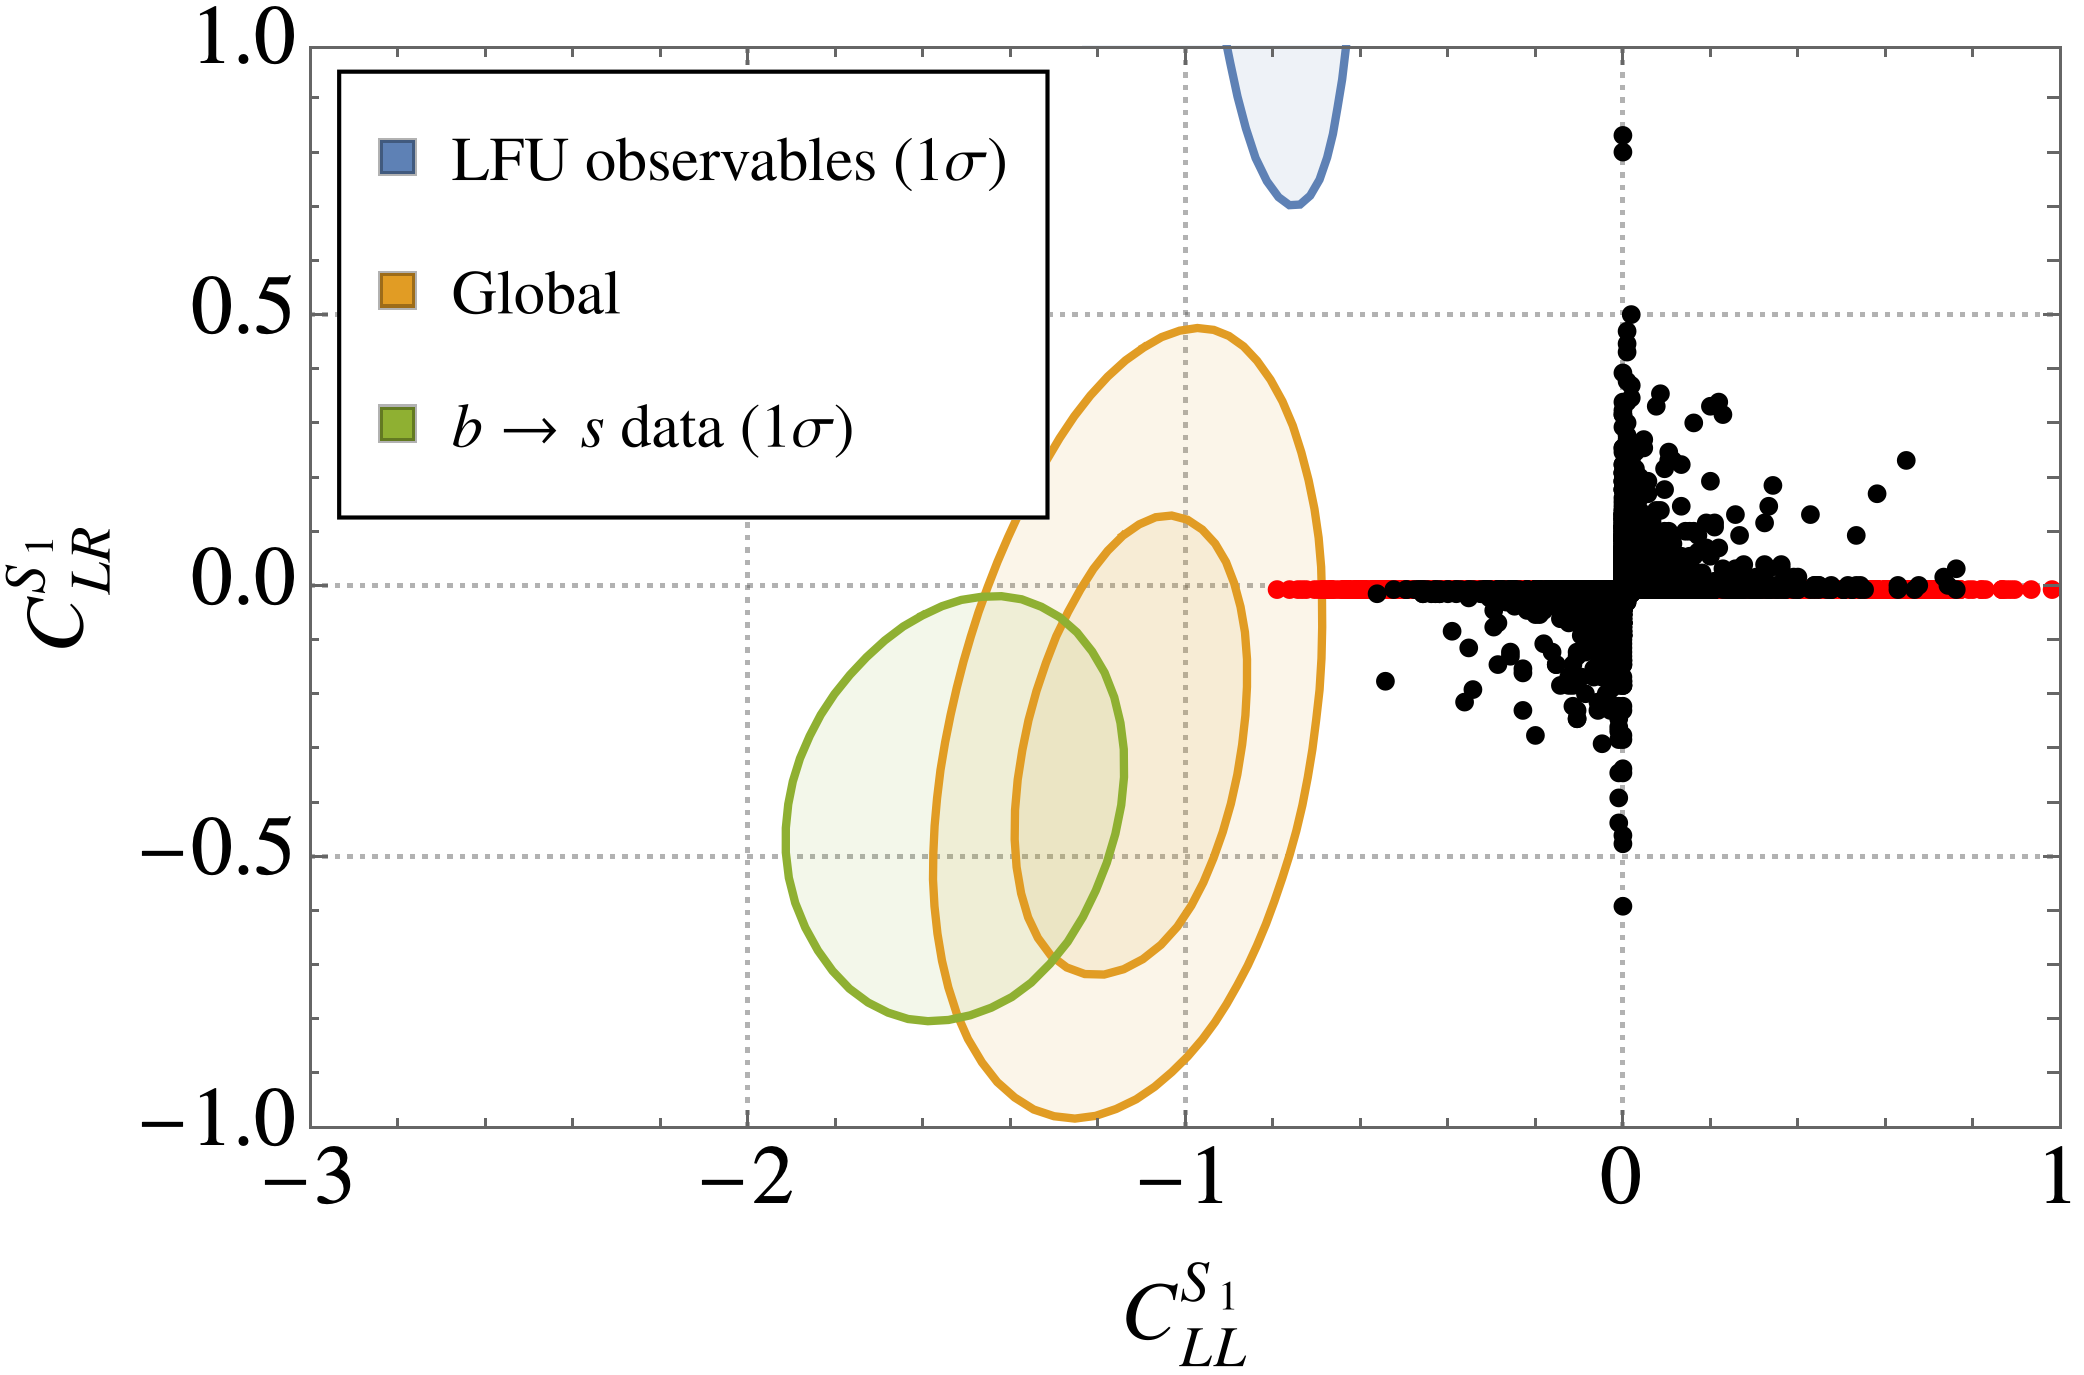
\includegraphics[width=0.7\linewidth]{newcllclr.png}
    \subcaption[The results of scan I (black) and scan II (red) projected onto
    the $C_{LL}^{S_{1}}$--$C_{LR}^{S_{1}}$ plane.]{The results of scan I (black)
      and scan II (red) projected onto the $C_{LL}^{S_{1}}$--$C_{LR}^{S_{1}}$
      plane. The contours are those of Fig.~\ref{fig:ch1-c9-c10-fit} projected
      onto the chiral basis, originally from Ref.~\cite{Aebischer:2019mlg}. The
      blue contours represent the fit to only LFU observables, the green the fit
      to the other $b \to s$ data, while the global fit contours are shown in
      orange. The model can alleviate the tensions in LFU observables to just
      shy of the $1\sigma$ region, a significant improvement on the SM. In this
      region, $C_{LR}^{S_{1}} \approx 0$, implying a suppression of the
      $y_{2r}$. Agreement with only the LFU observables is not as good.\vspace{1em}}
    \label{fig:ch3-cllclrpts1}
  \end{minipage}
  \begin{minipage}[t]{.49\linewidth}
    \centering 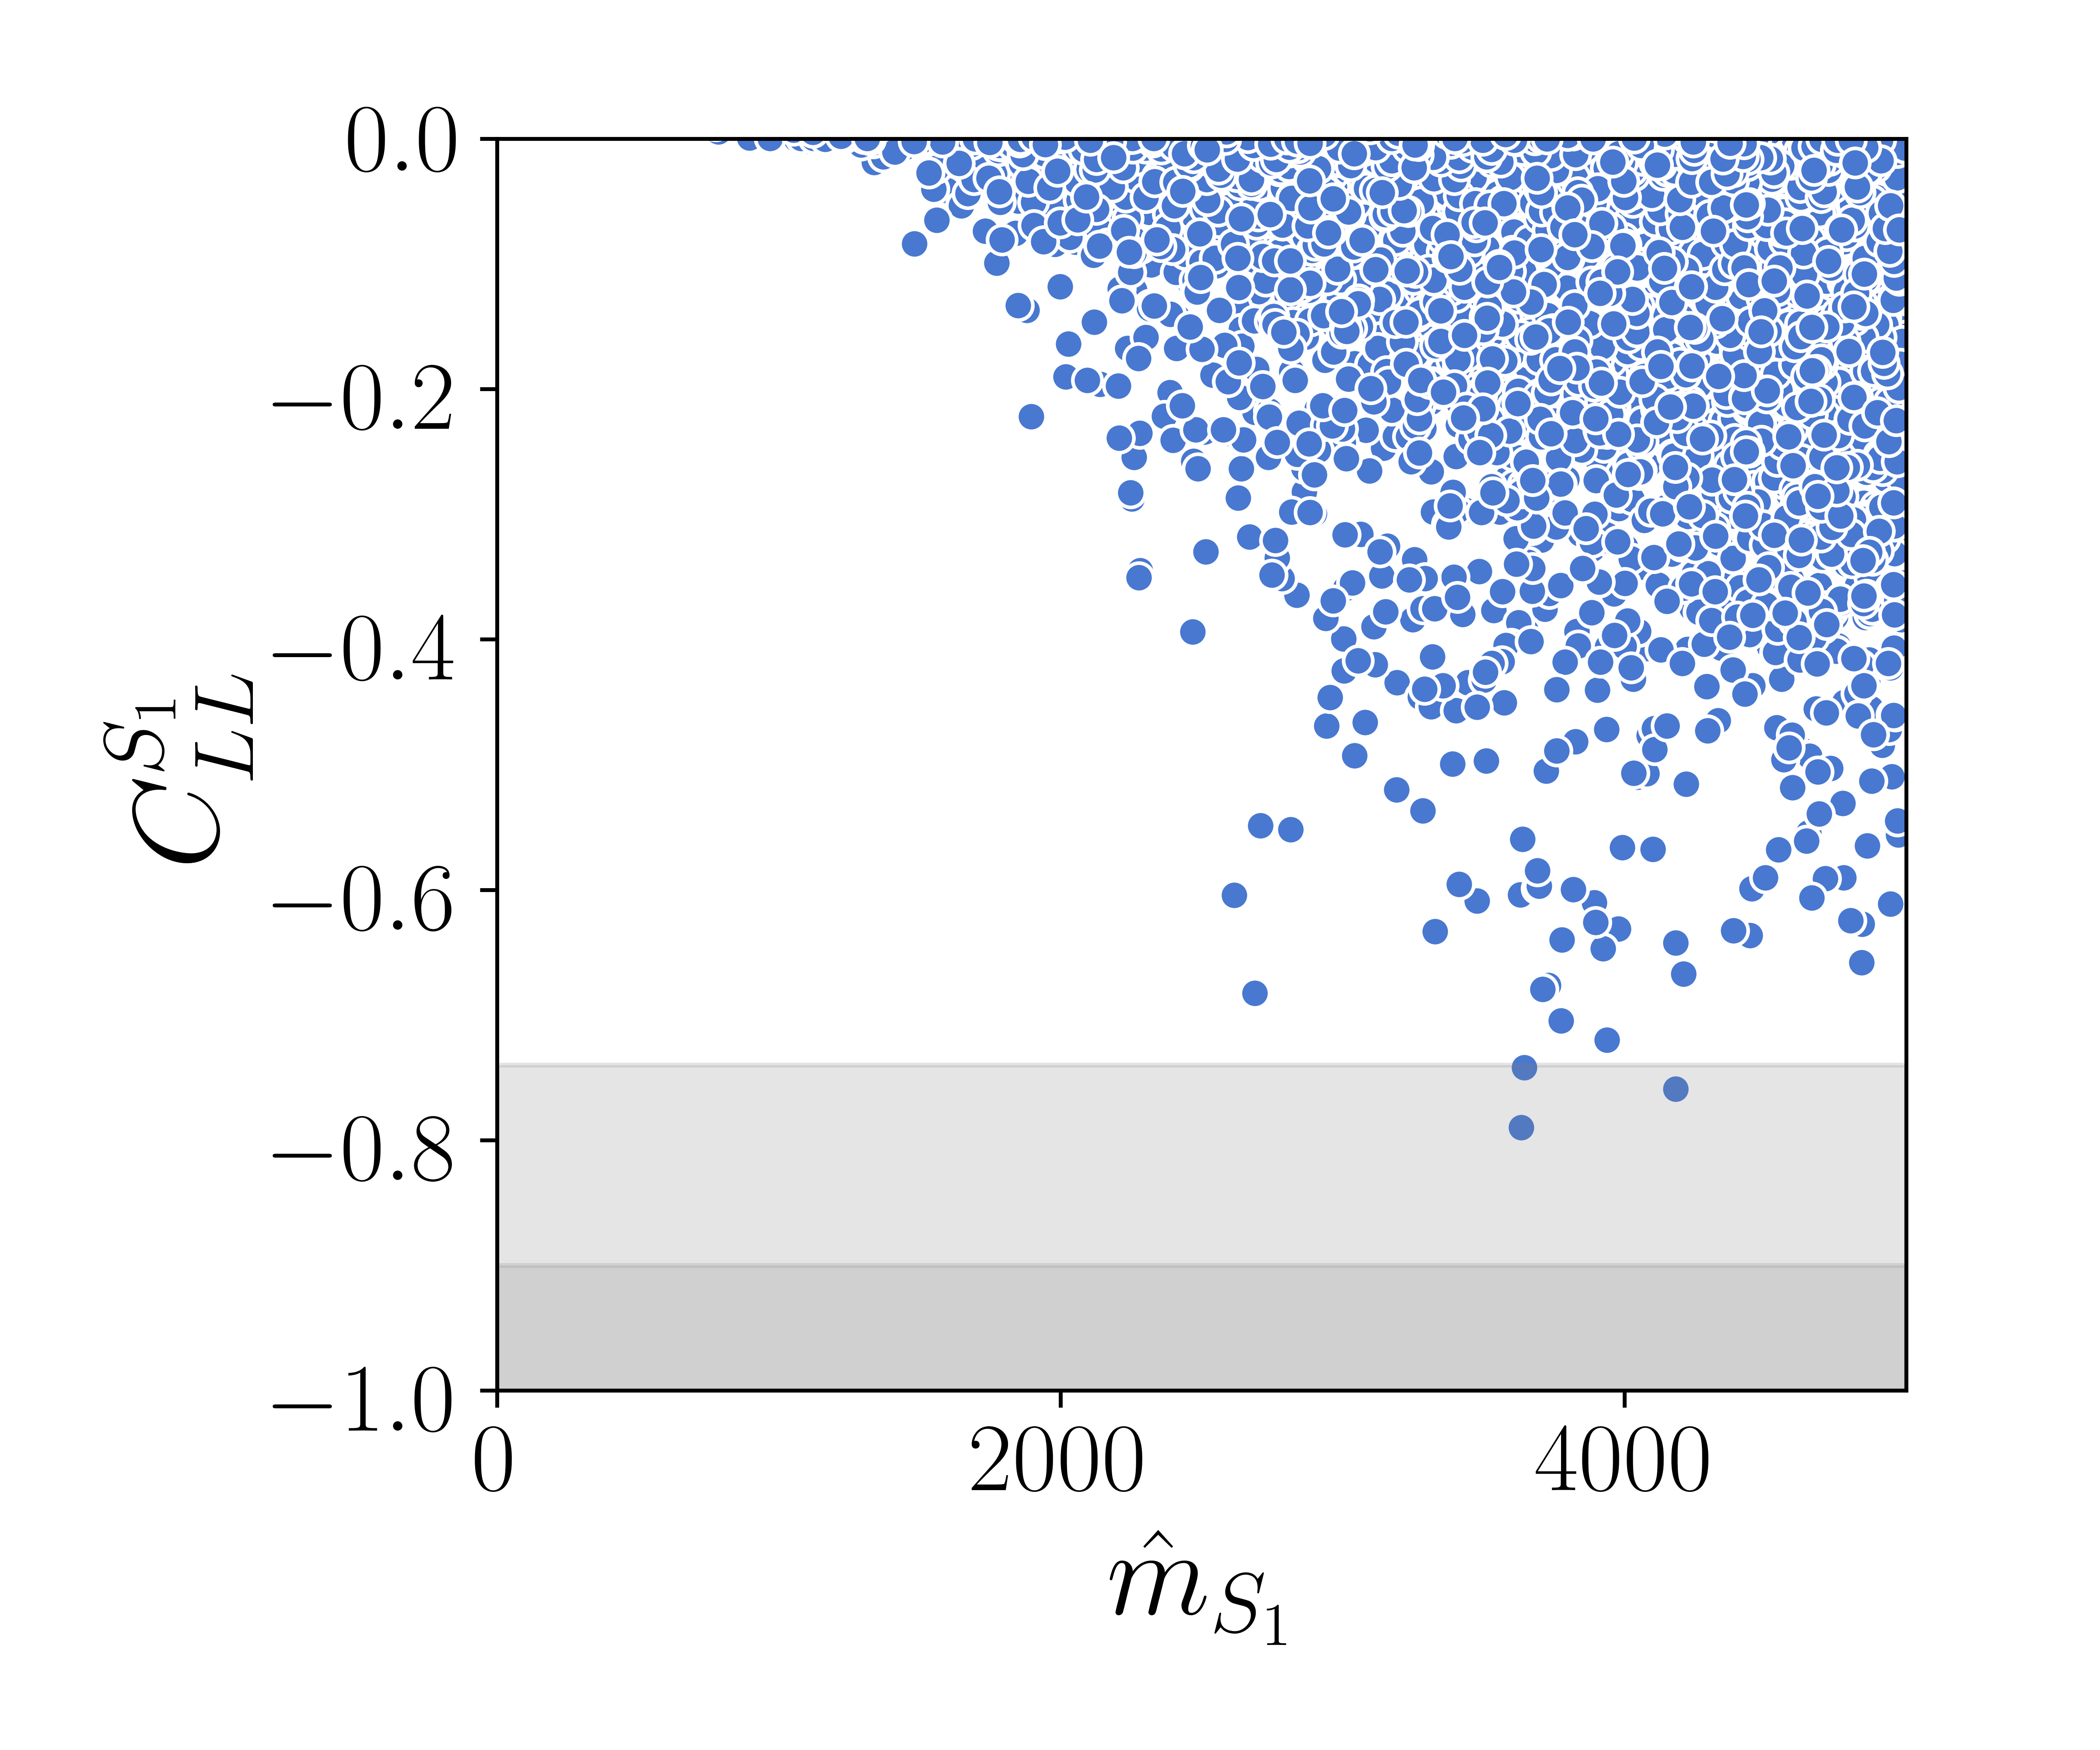
\includegraphics[width=\linewidth]{new_cllm.png}
    \subcaption[A scatter plot showing the results of scan II projected onto the
      $C_{LL}^{S_{1}}$--$\hat{m}_{S_{1}}$ plane.]{A scatter plot showing the results of scan II projected onto the
      $C_{LL}^{S_{1}}$--$\hat{m}_{S_{1}}$ plane. Yellow points imply SM-like values
      for $R_D$ and $R_{D^{*}}$. The constraints imposed by $D^0 \to \mu \mu$,
      $D^+ \to \pi^+ \mu \mu$ and $Z \to \mu \bar{\mu}$ disfavor light
      leptoquark masses.}
    \label{fig:ch3-cllm}
  \end{minipage}
  \hfill
  \begin{minipage}[t]{.49\linewidth}
    \centering 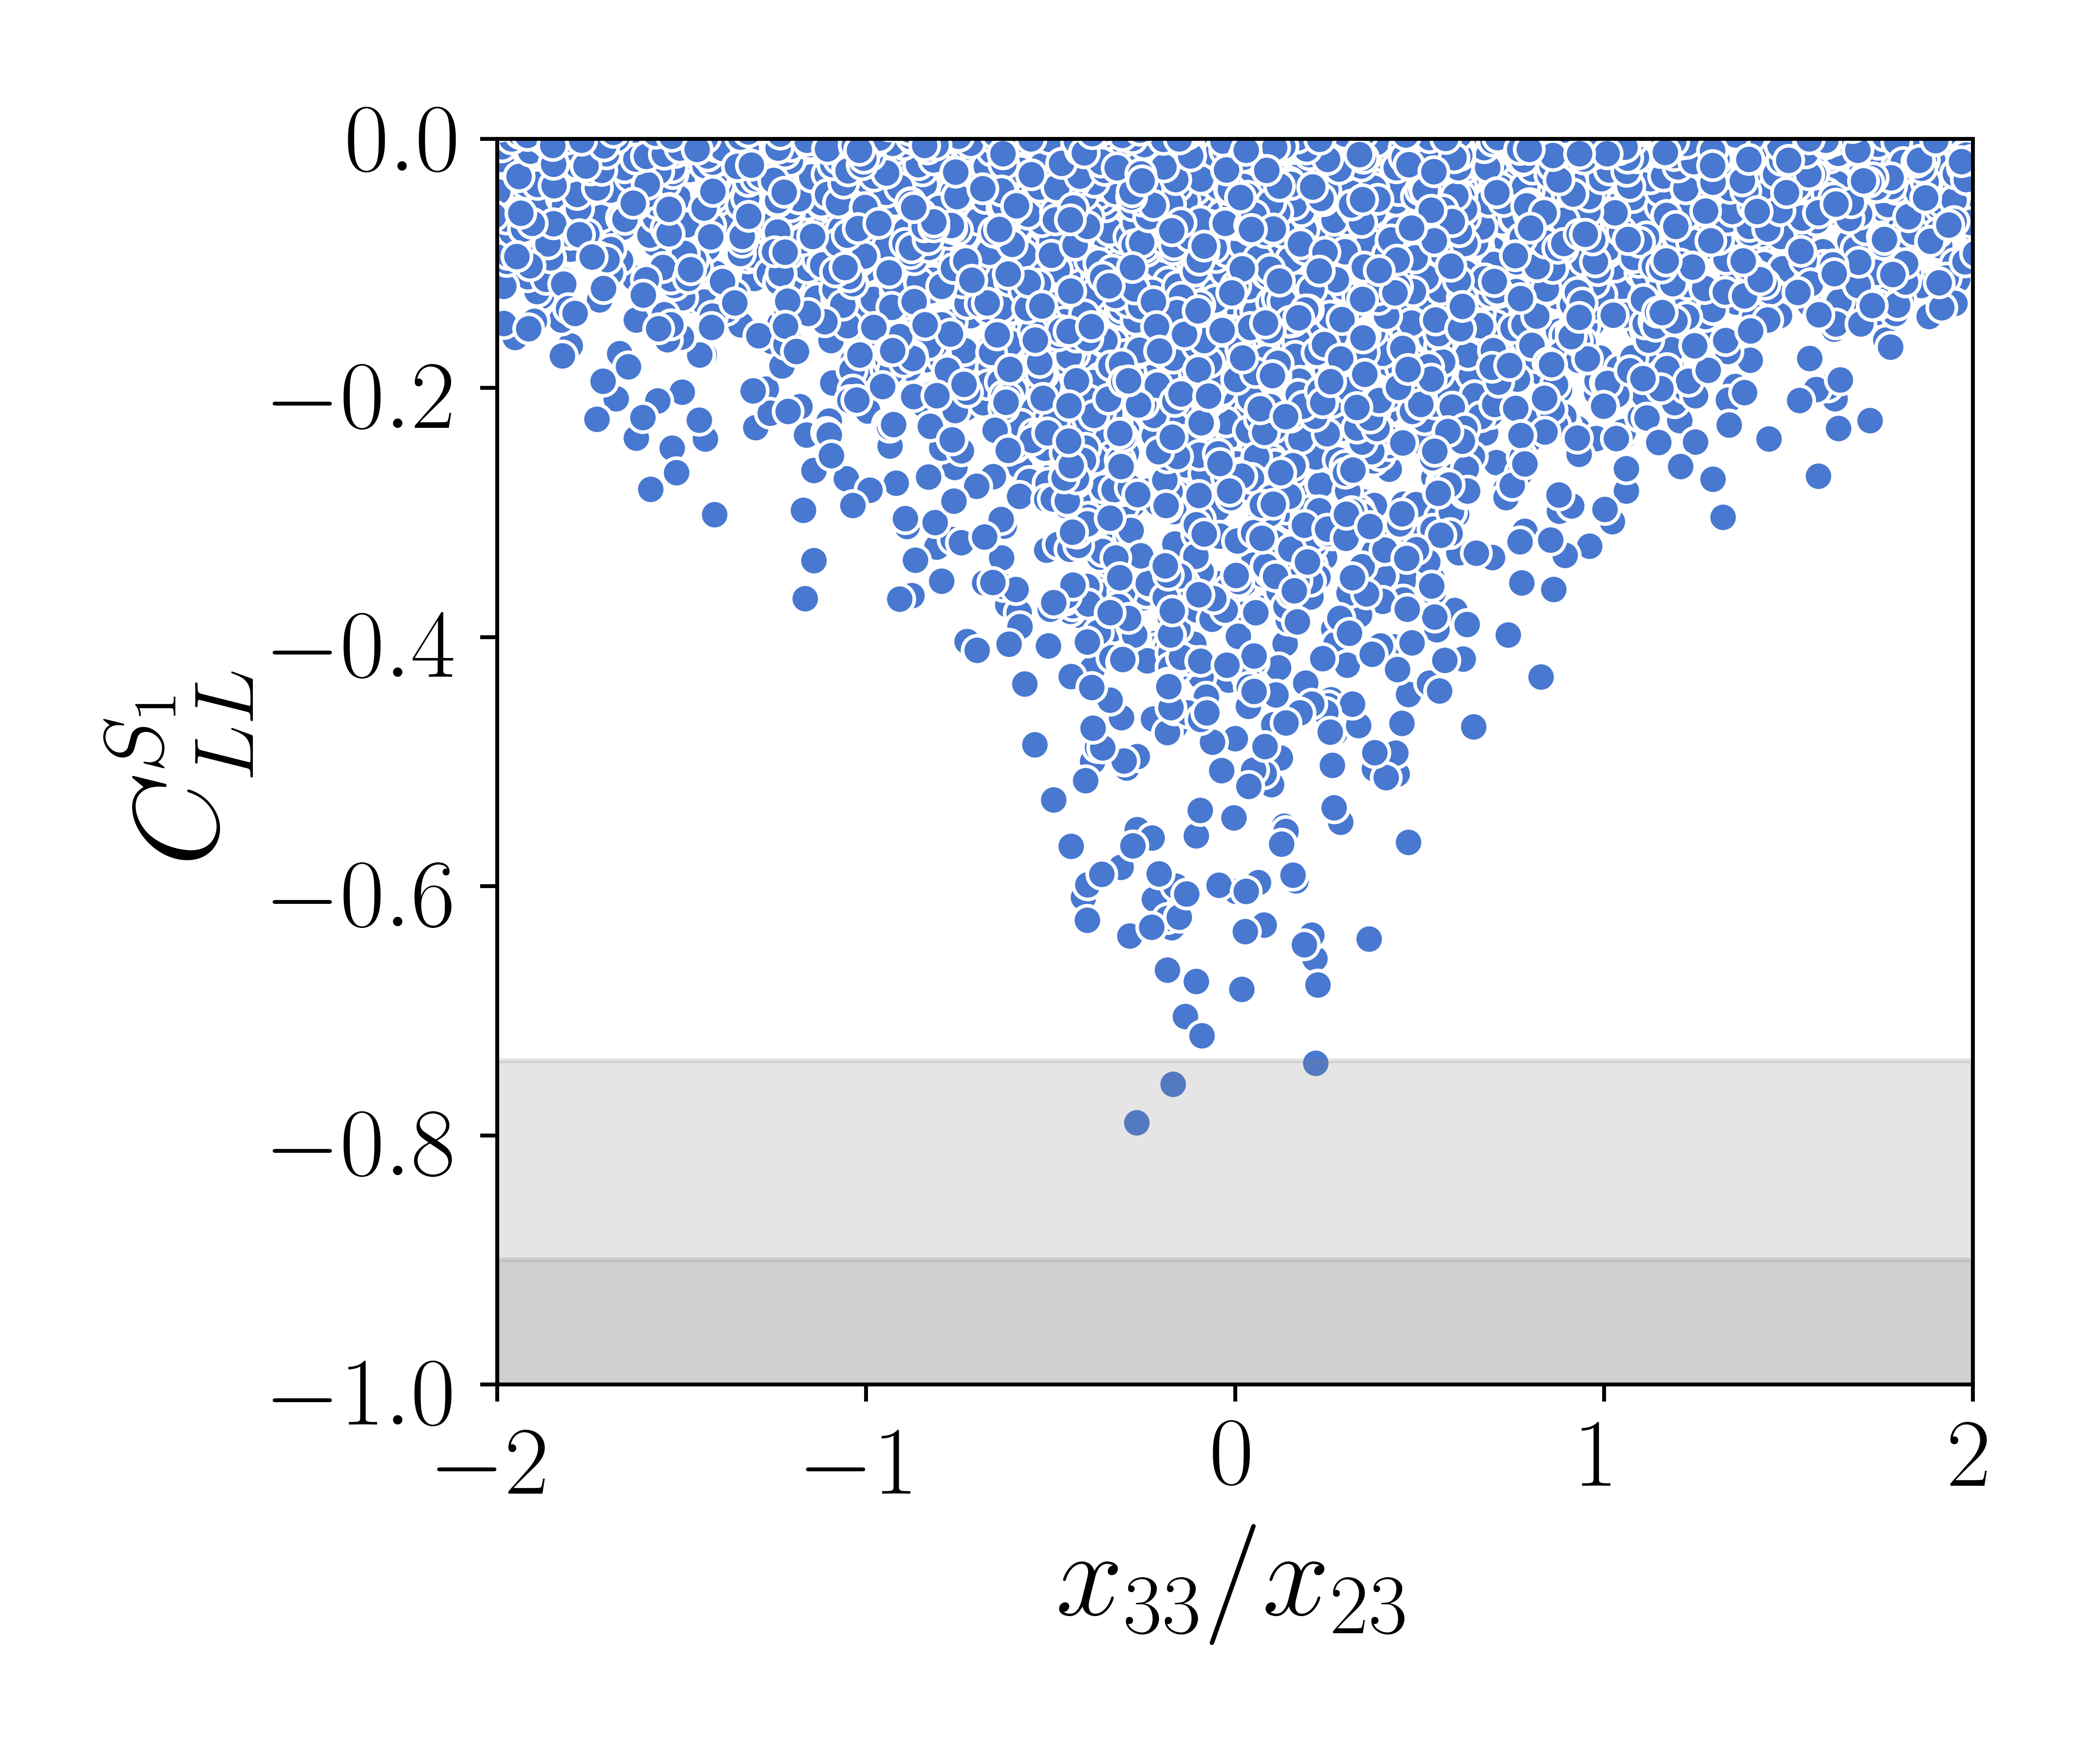
\includegraphics[width=\linewidth]{new_x33x23rat.png}
    \subcaption[A scatter plot of $C_{LL}^{S_{1}}$ against the ratio
      $x_{33}/x_{23}$ for parameters subject to scan II.]{A scatter plot of $C_{LL}^{S_{1}}$ against the ratio
      $x_{33}/x_{23}$ for parameters subject to scan II. Again, yellow points
      correspond to SM-like $R_D$ and $R_{D^{*}}$. A large, negative value for
      $C_{LL}^{S_{1}}$ requires $|x_{23}| > |x_{33}|$ to keep LFV $\tau \to \mu$
      observables at bay.}
    \label{fig:ch3-x33x32rat}
  \end{minipage}
  \caption[The key results probing the extent to which the model can explain the
  tensions in the $b \to s$ data.]{The key results probing the extent to which
    the model can explain the tensions in $b \to s$ data. Significant
    improvement from the SM is possible for leptoquark masses between $3$ and
    $\SI{5}{\TeV}$, $|x_{23}| > |x_{33}|$ and suppressed $y_{2r}$. The grey
    areas in (b) and (c) are the $1$ and $2\sigma$ allowed regions for
    $C_{LL}^{S_{1}}$.}
  \label{fig:ch3-cllclrpts}
\end{figure}

\begin{figure}
    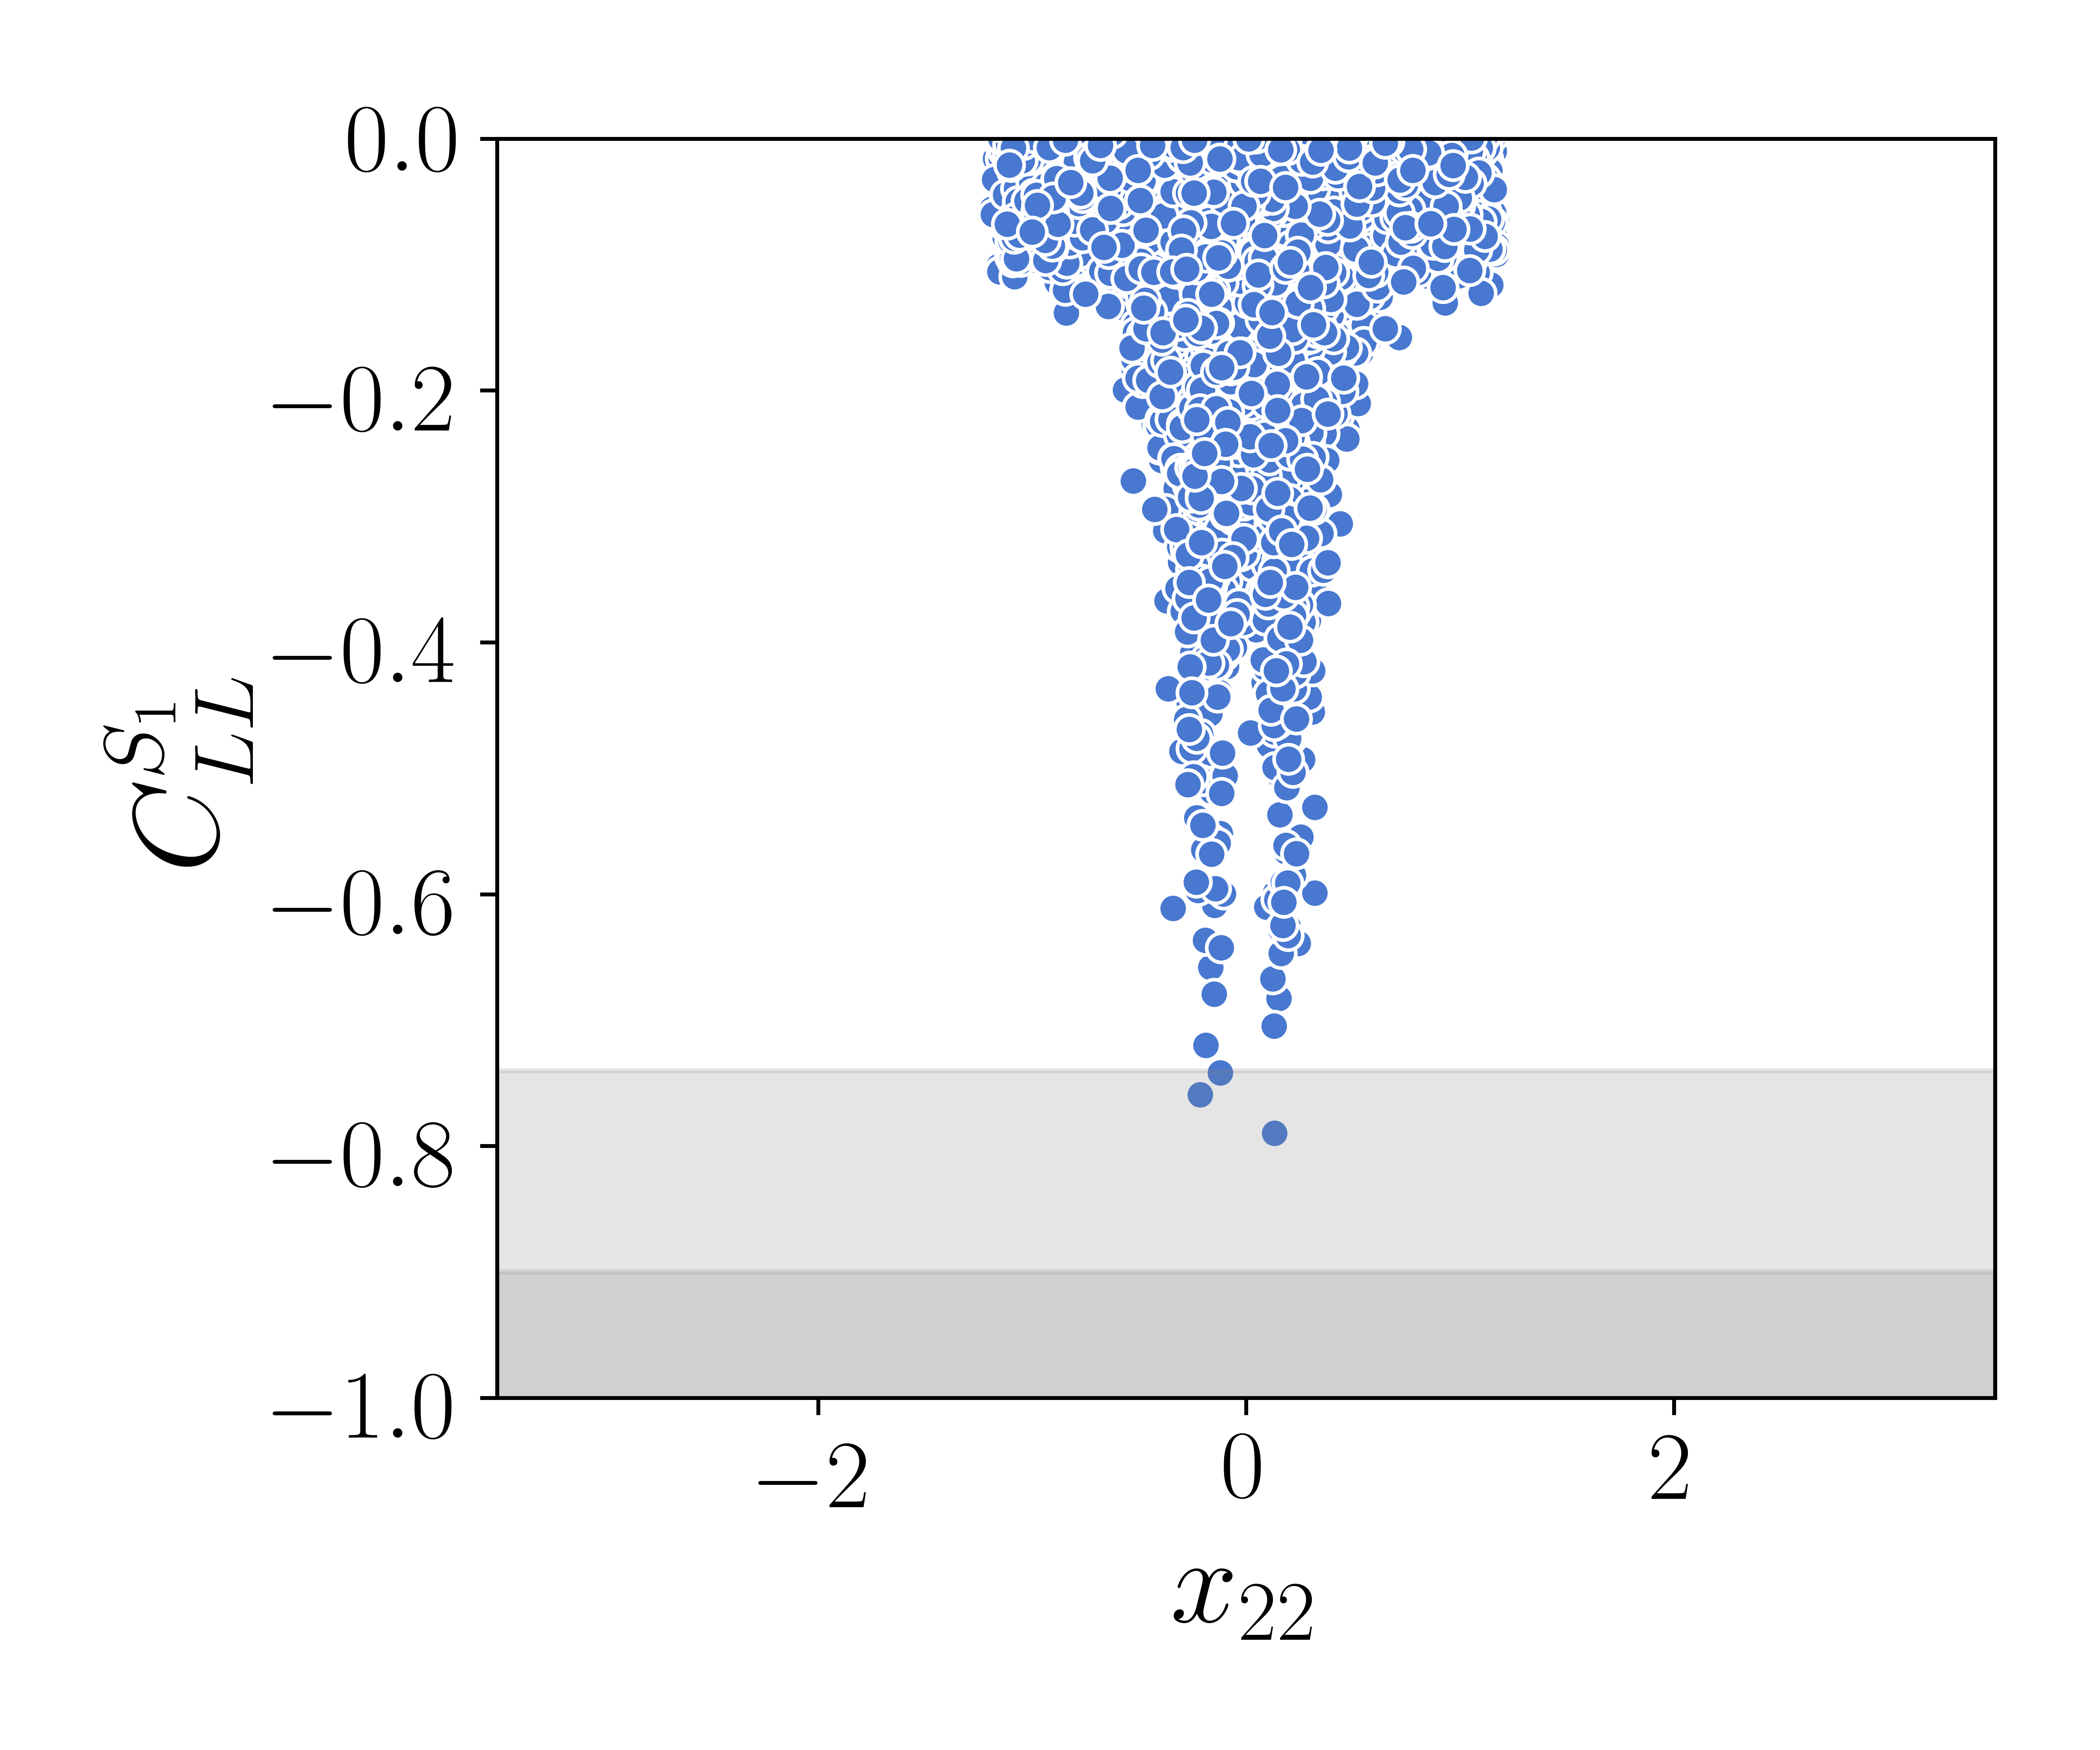
\includegraphics[width=0.49\textwidth]{new_cllx22.png} \hfill
    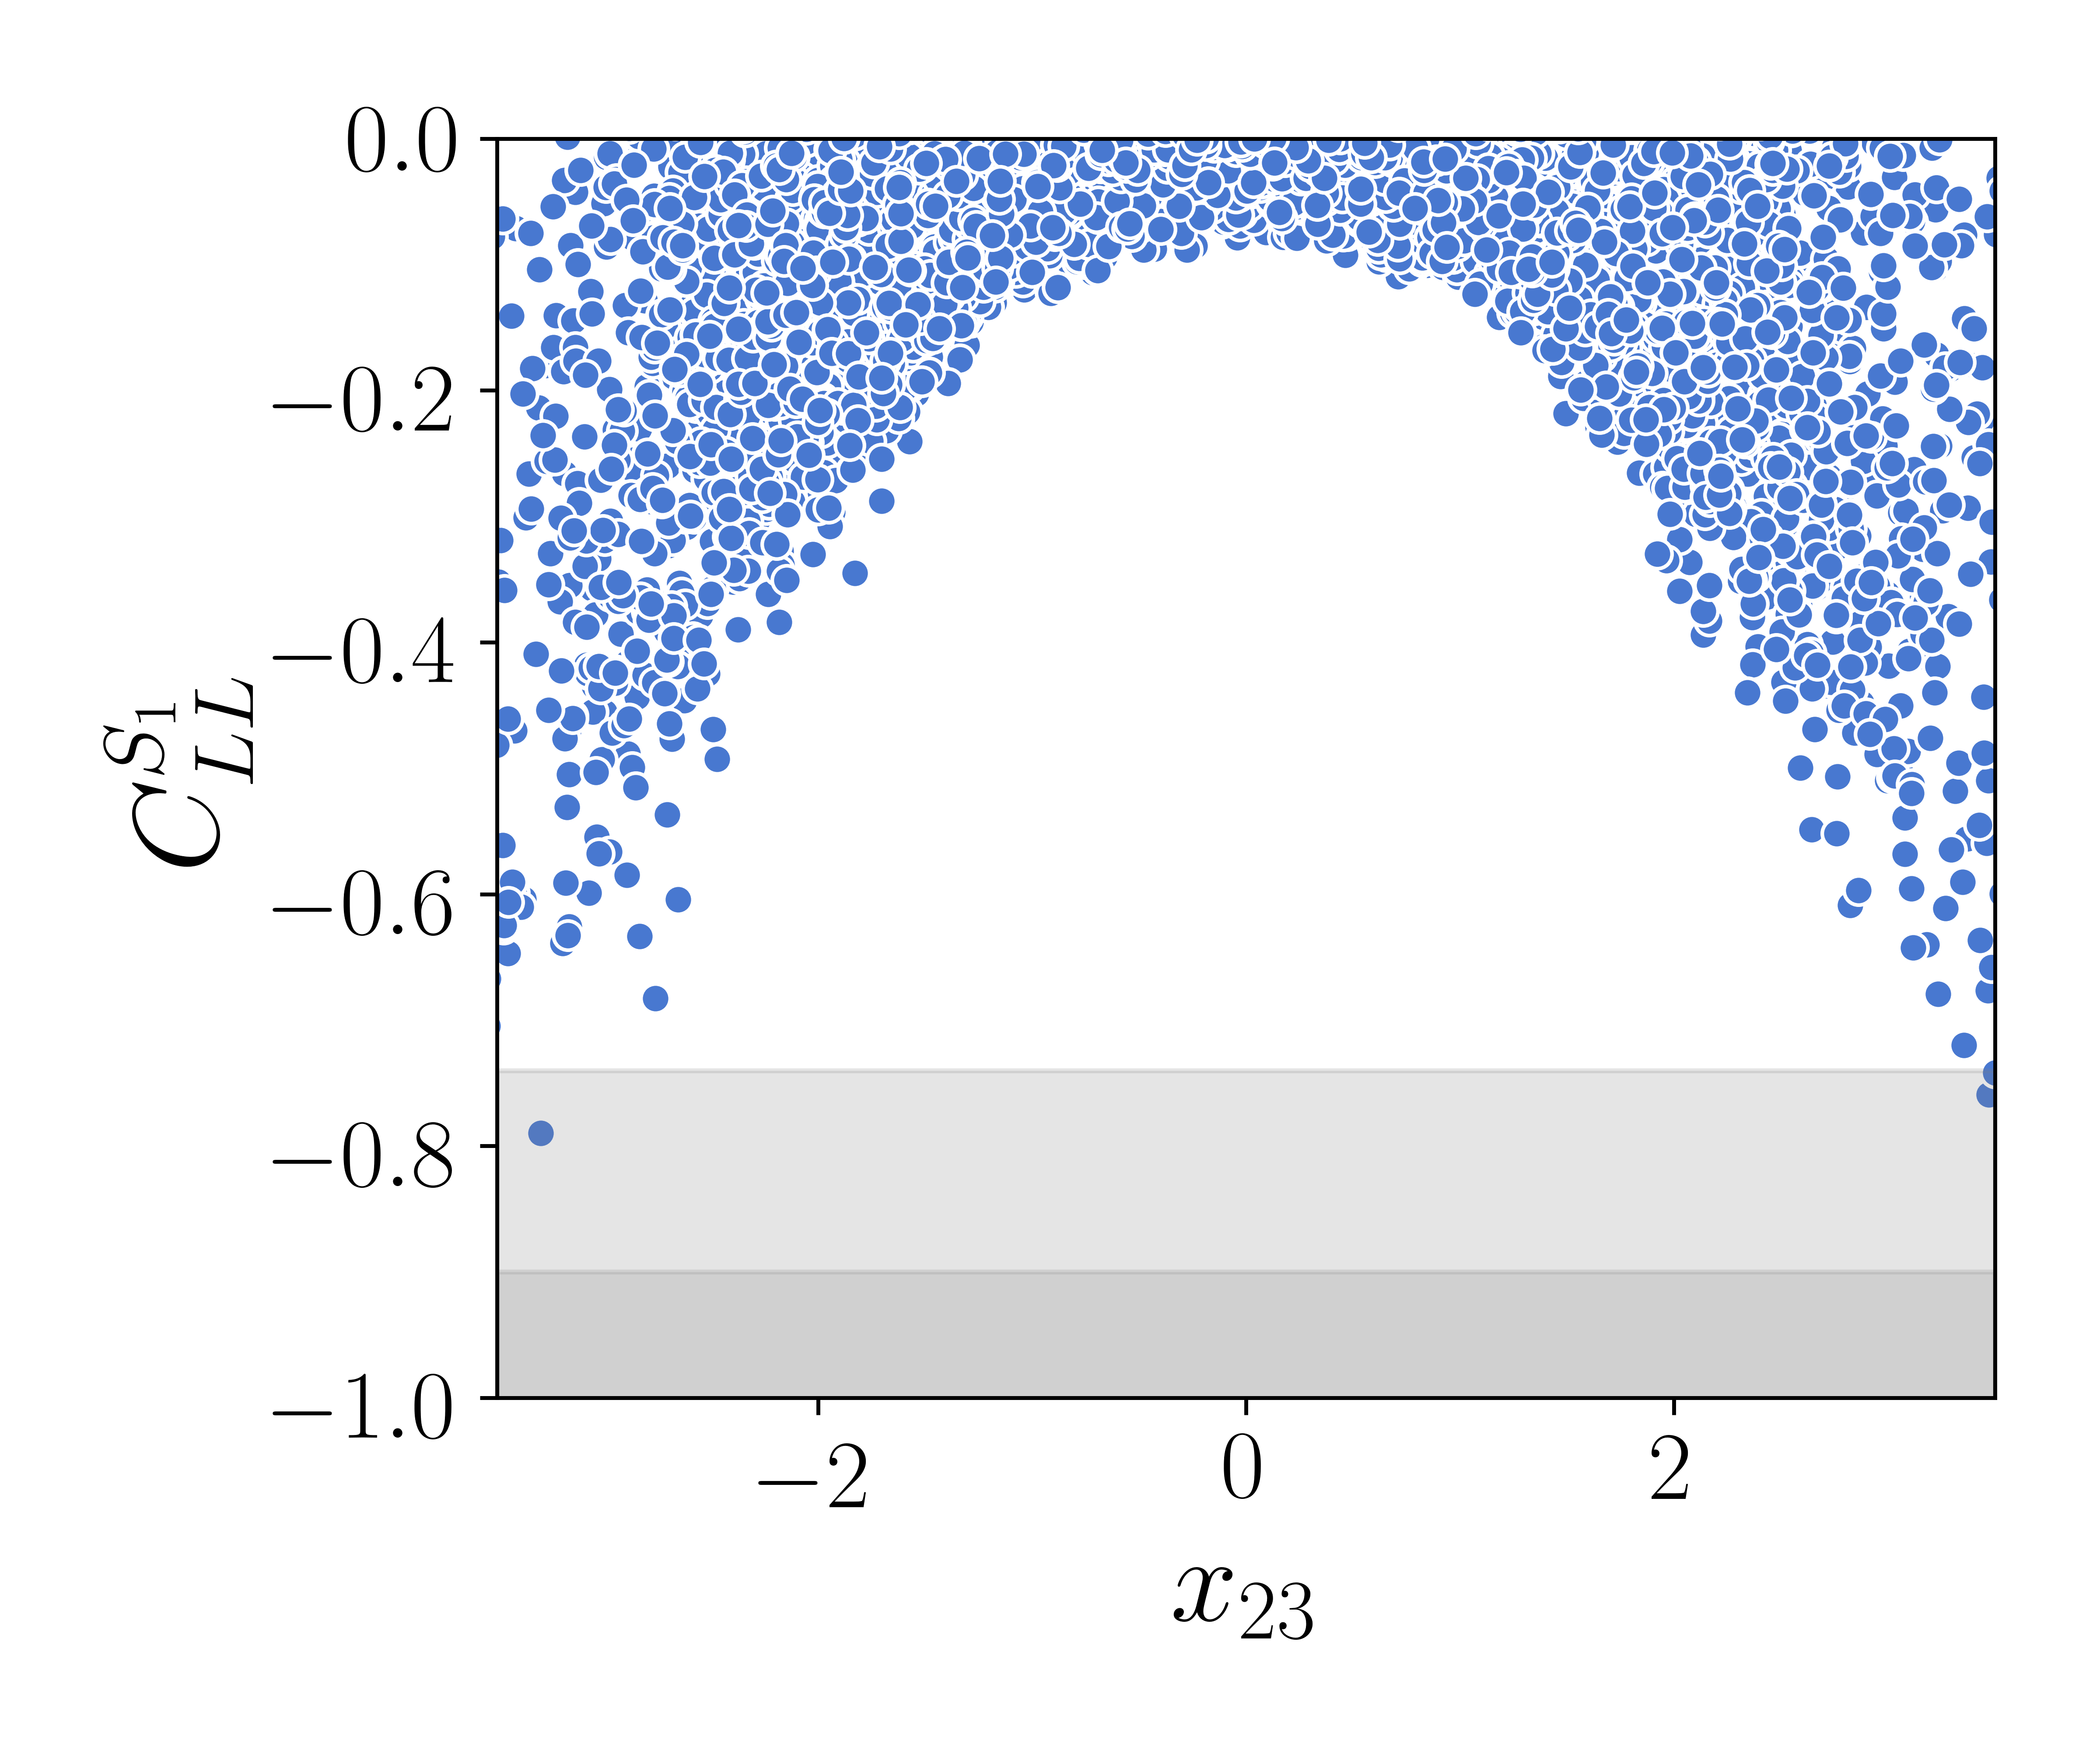
\includegraphics[width=0.49\textwidth]{new_cllx23.png} \\
    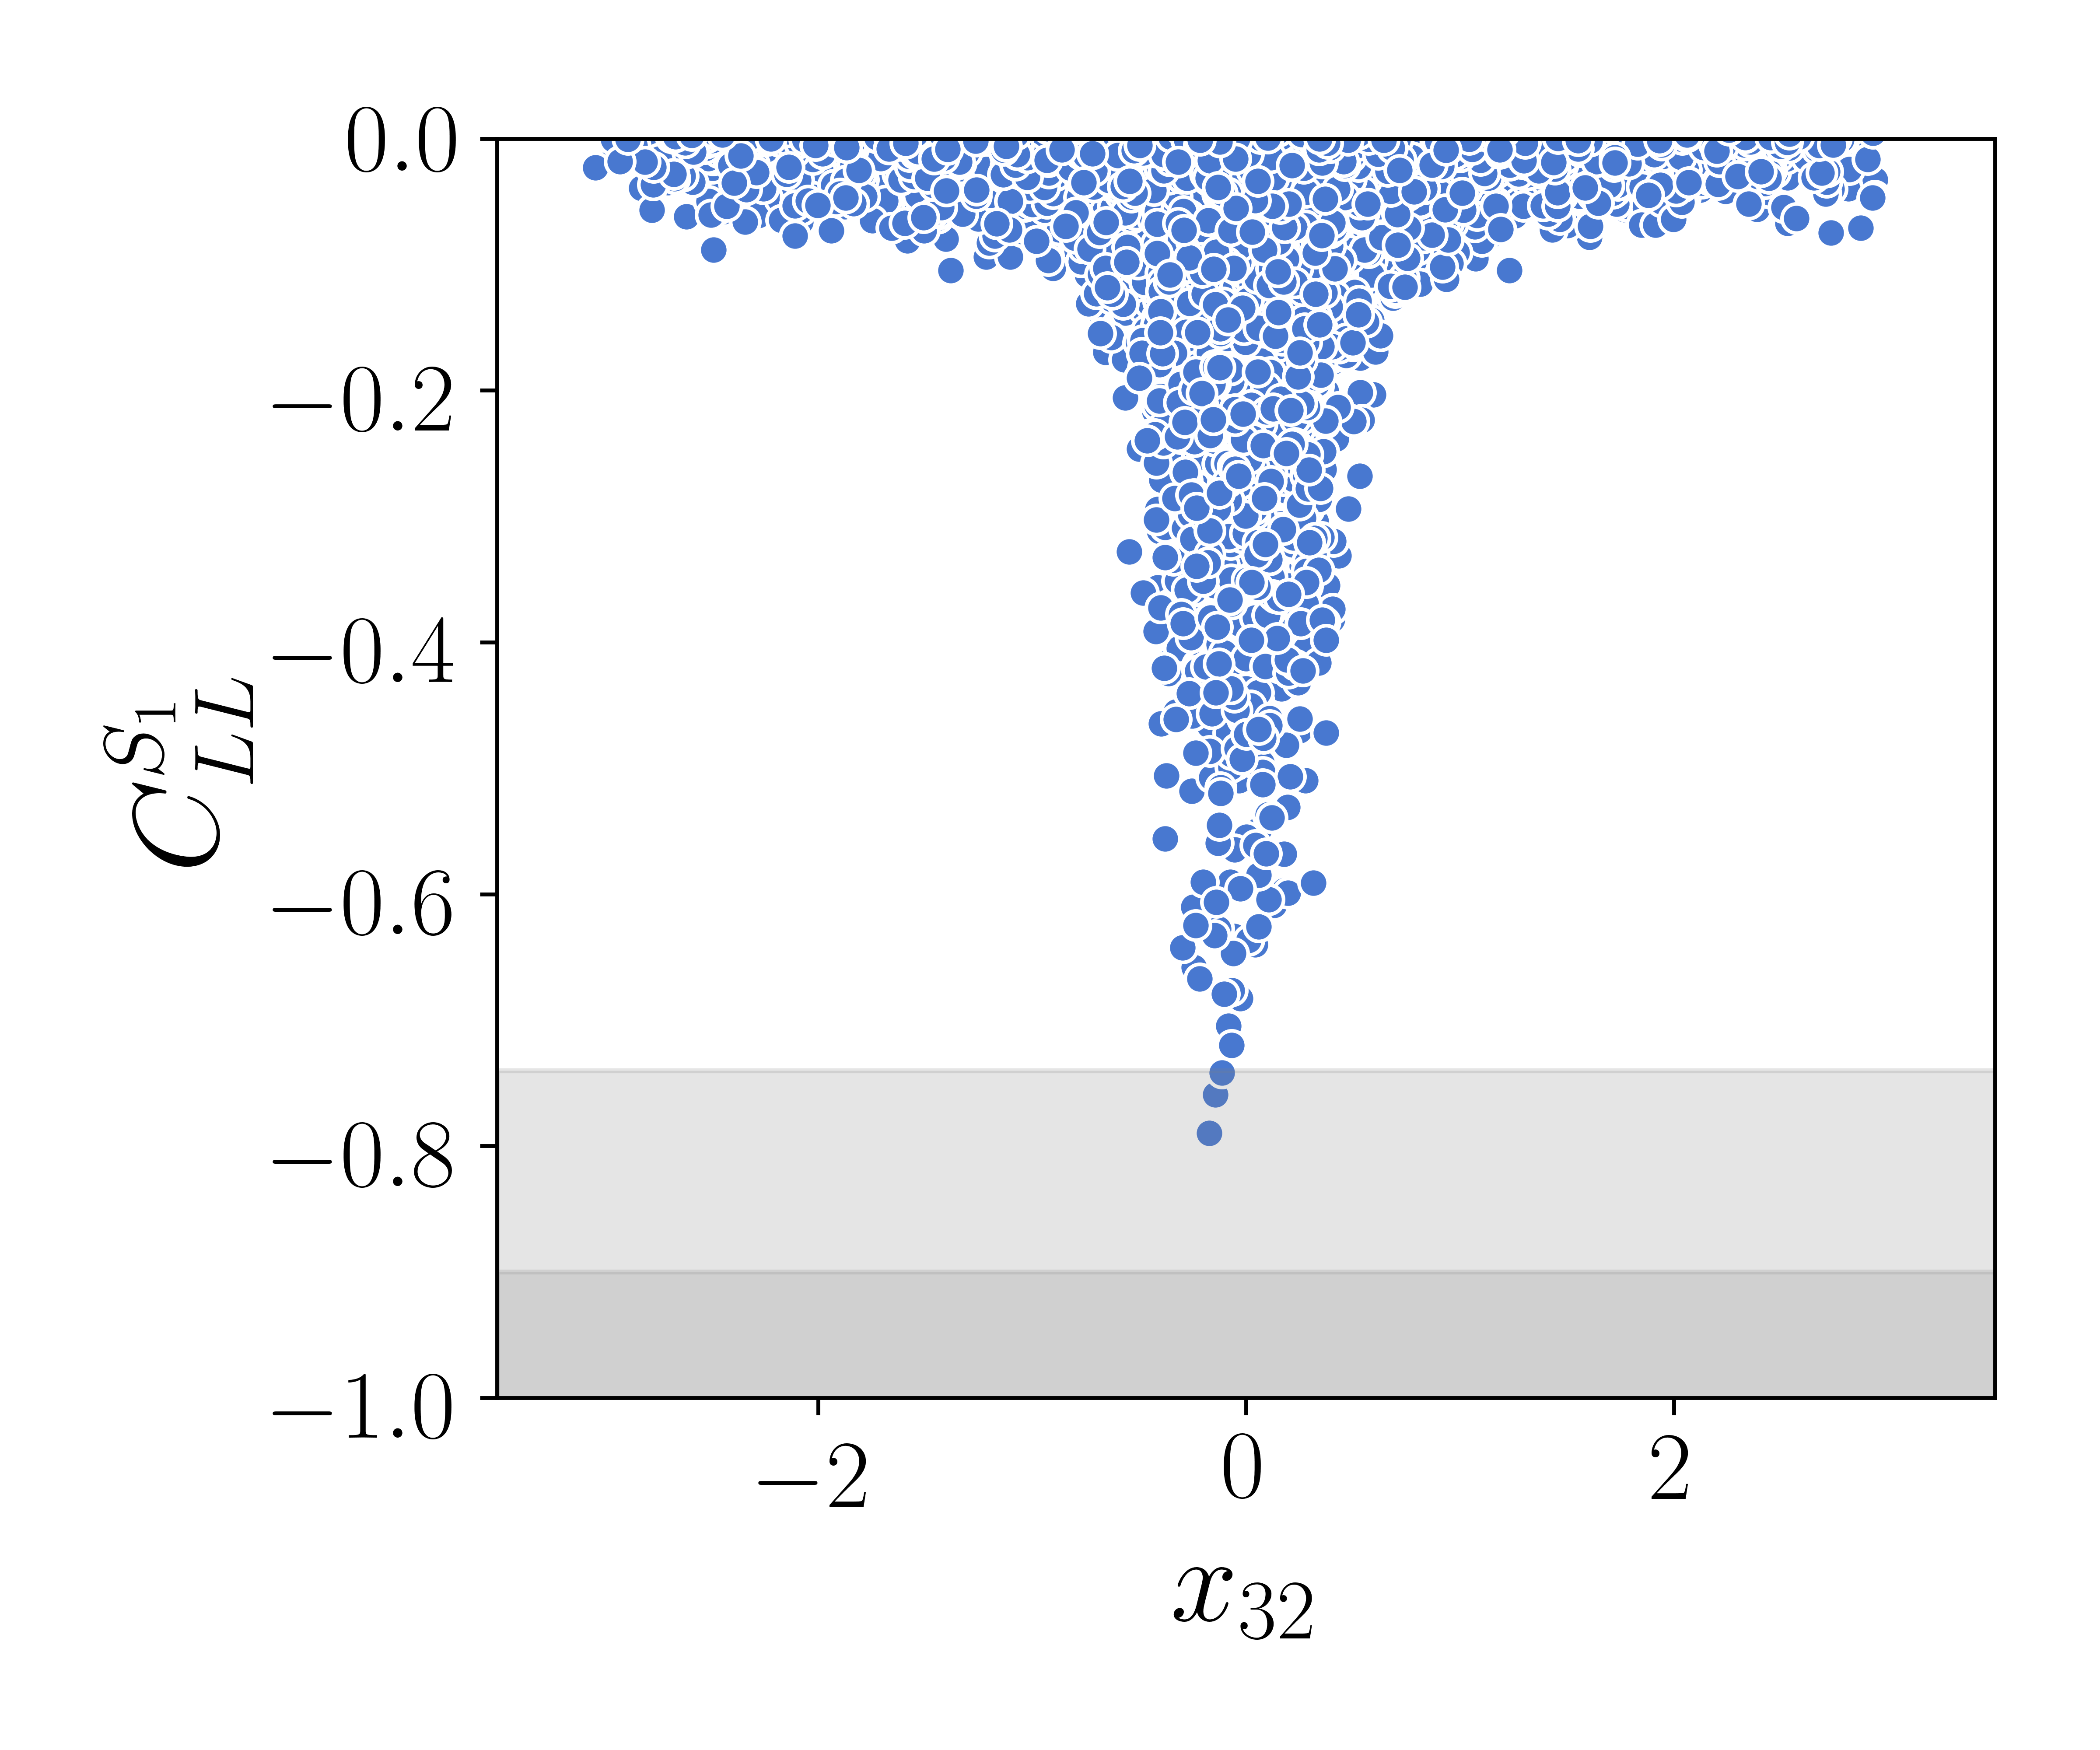
\includegraphics[width=0.49\textwidth]{new_cllx32.png} \hfill
    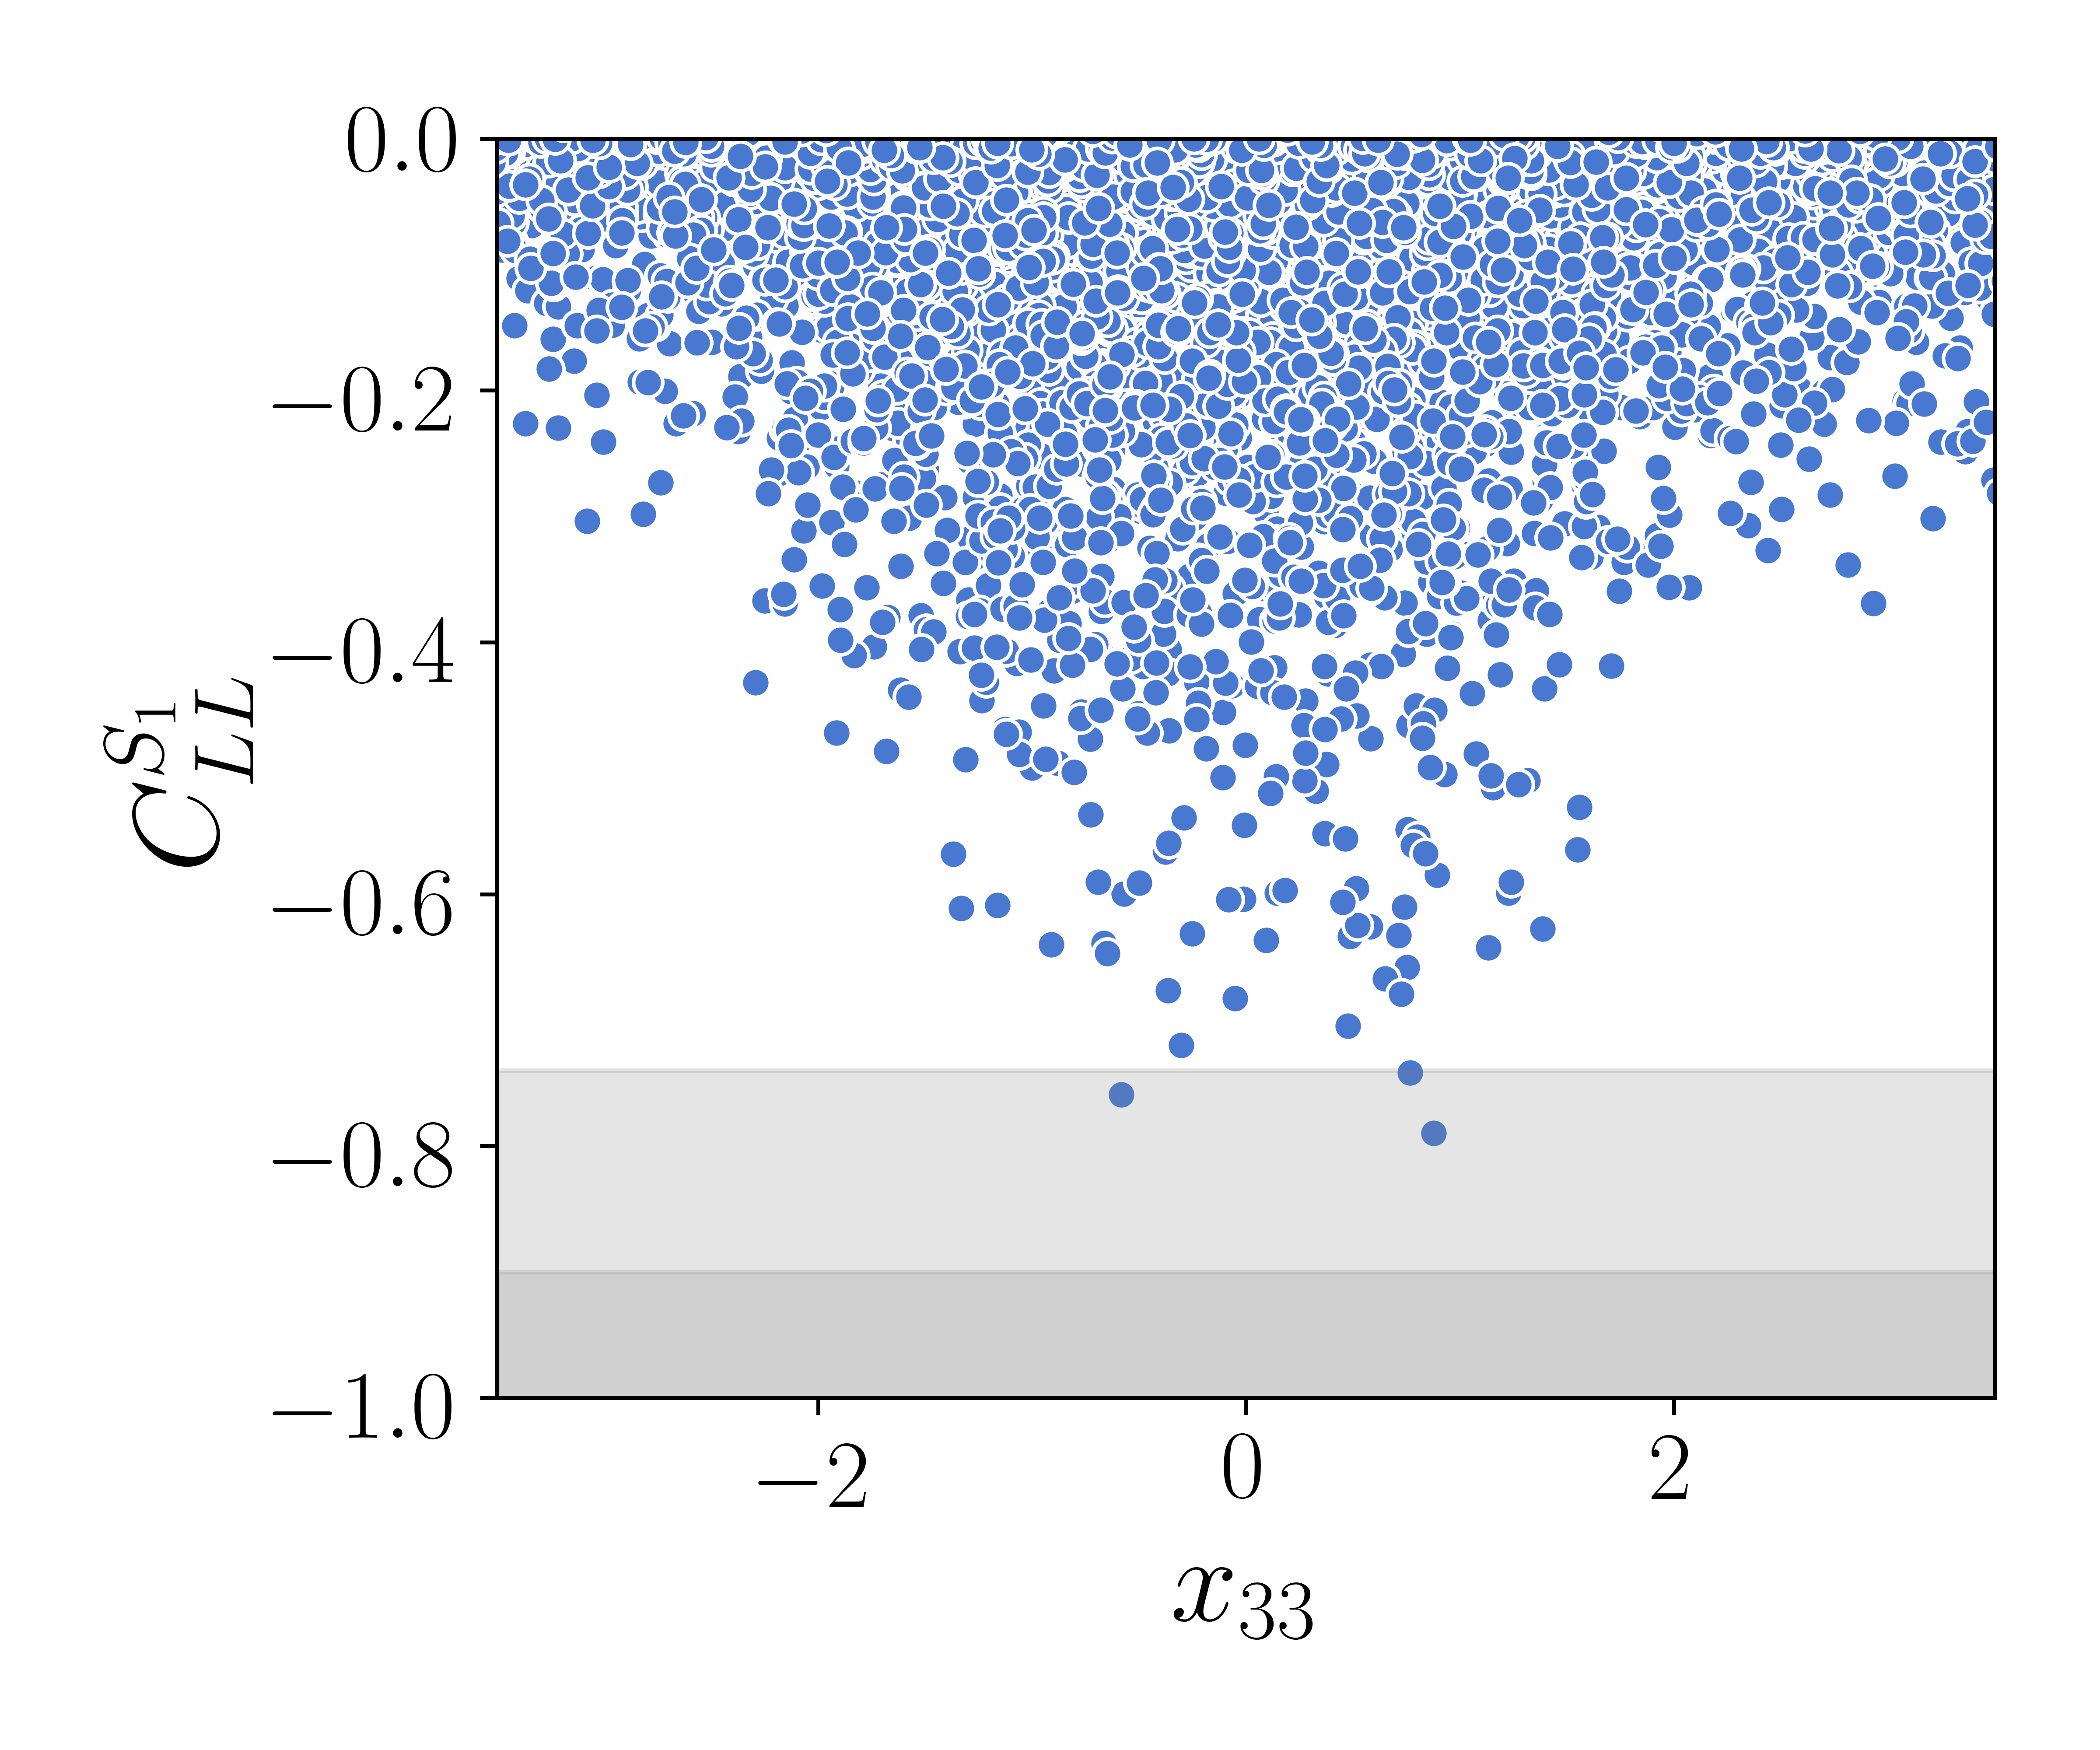
\includegraphics[width=0.49\textwidth]{new_cllx33.png}
    % 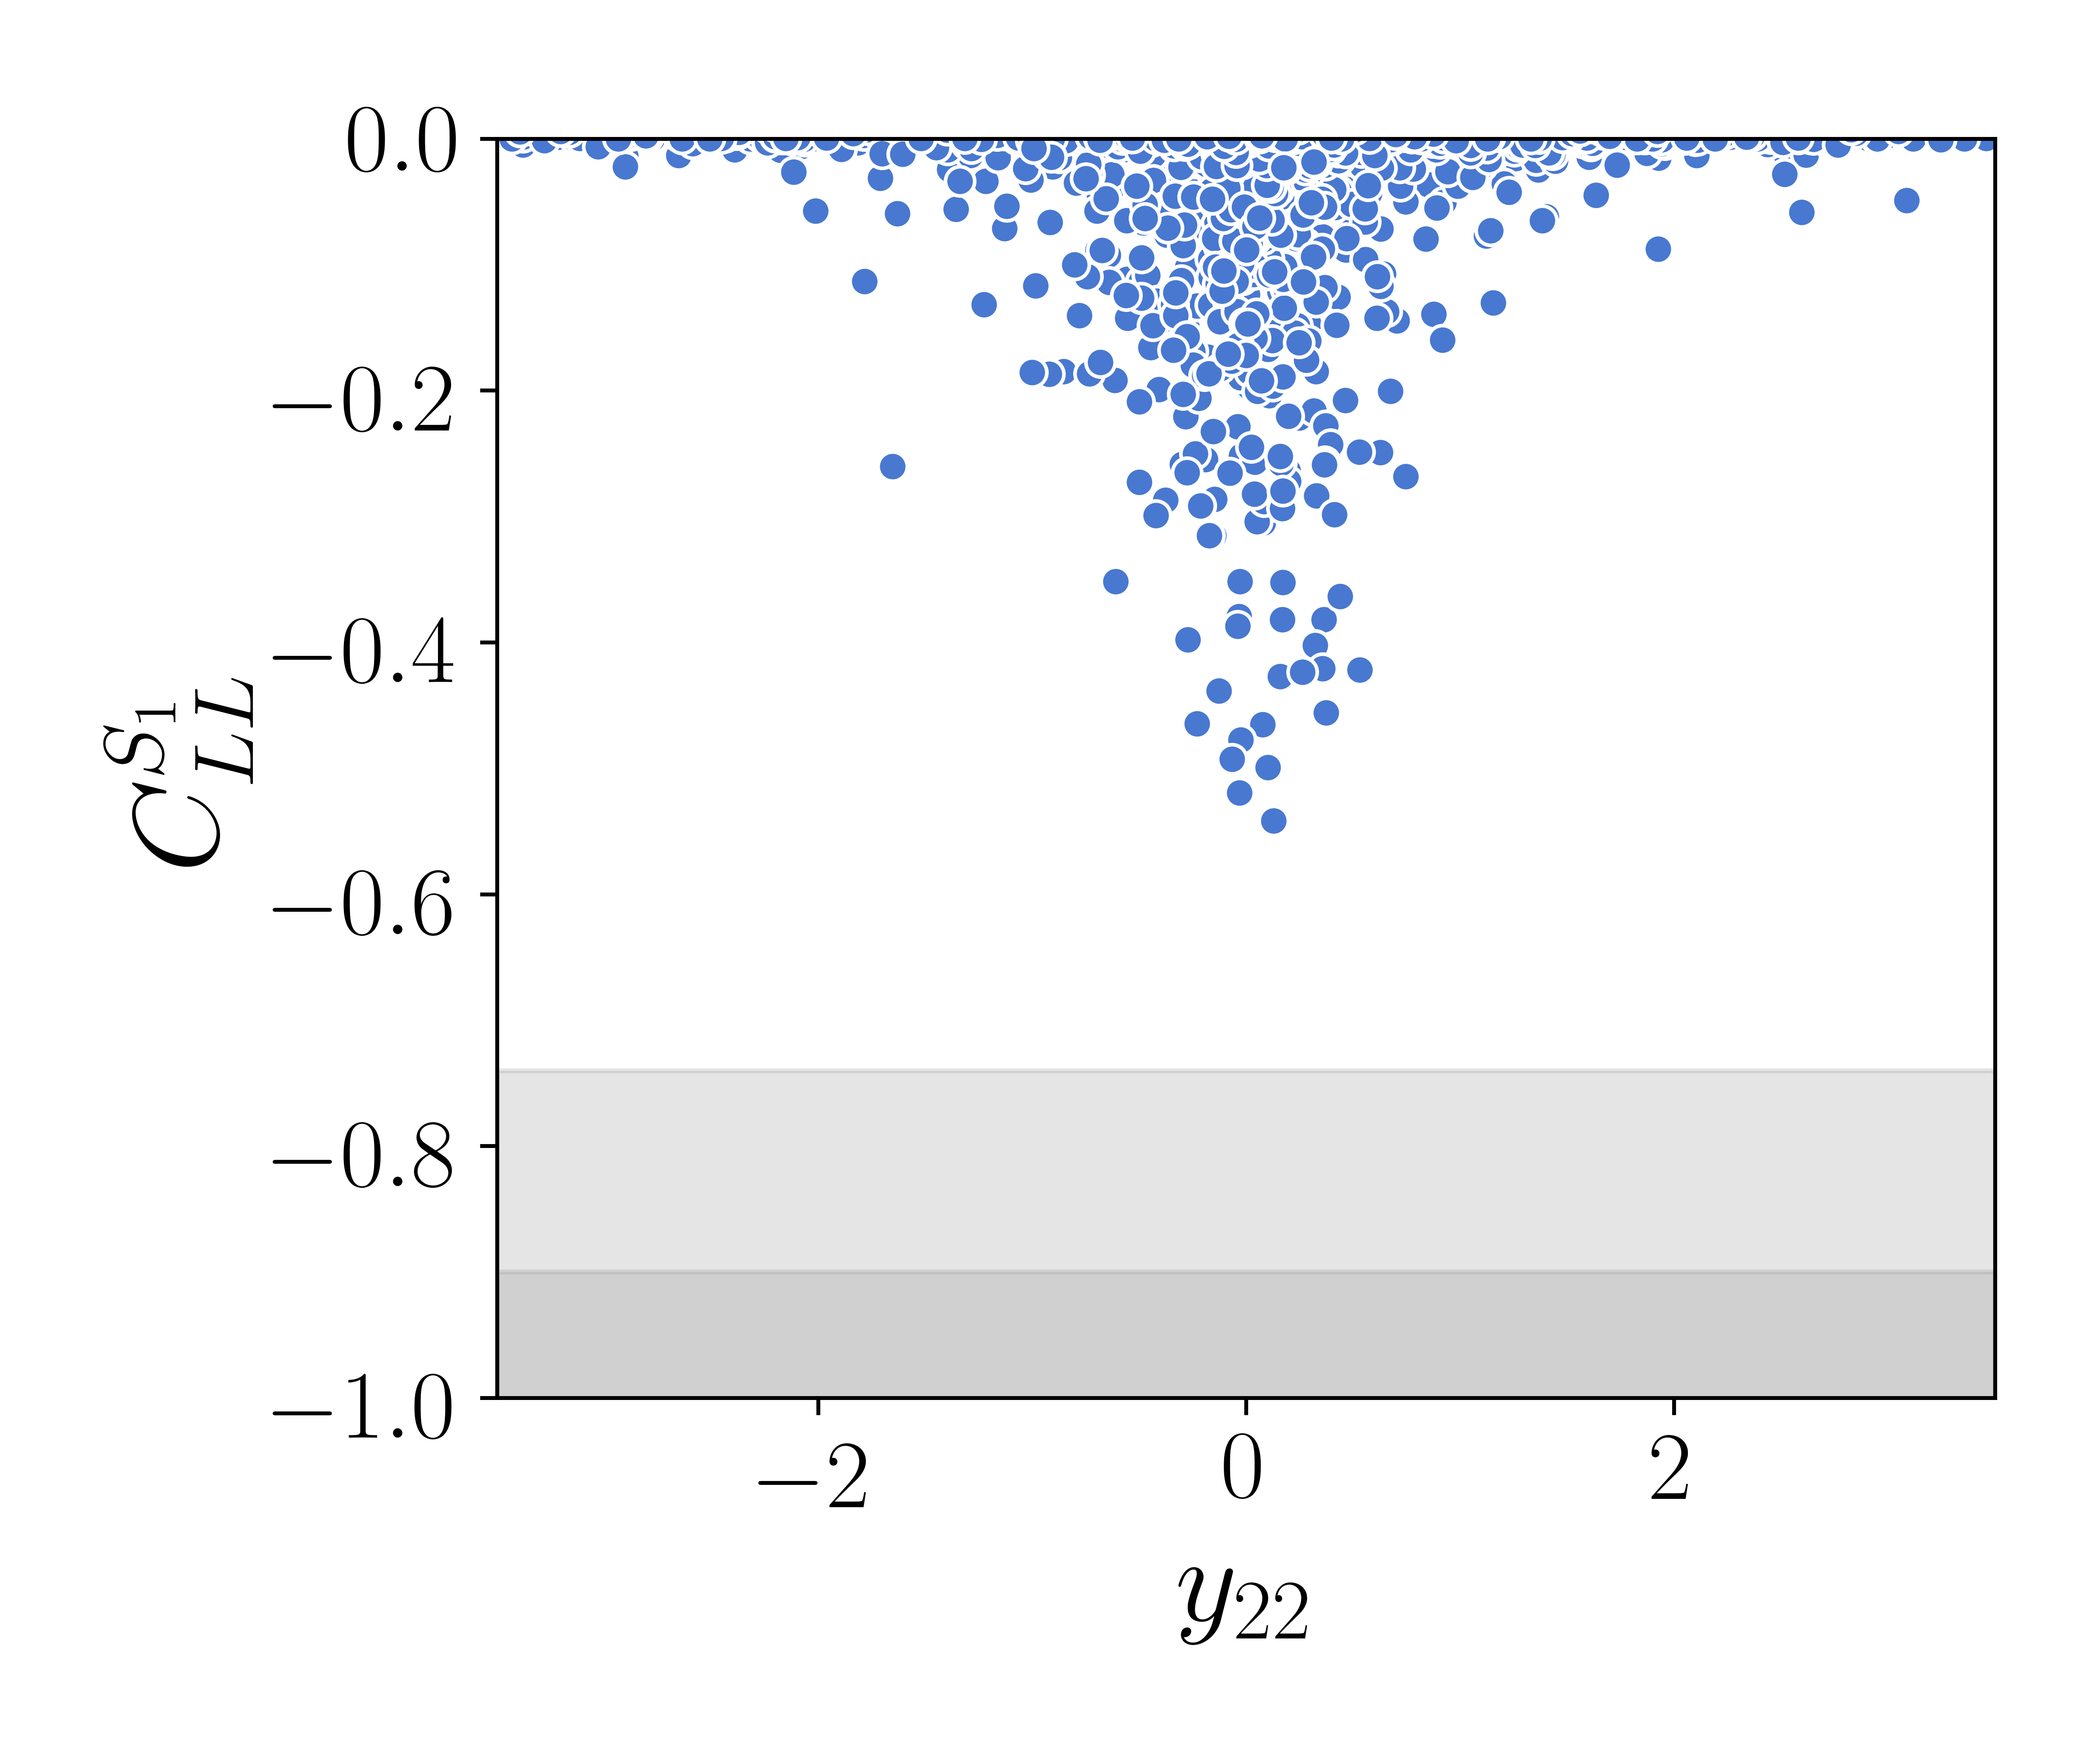
\includegraphics[width=0.40\textwidth]{new_clly22.png} \hfill
    % 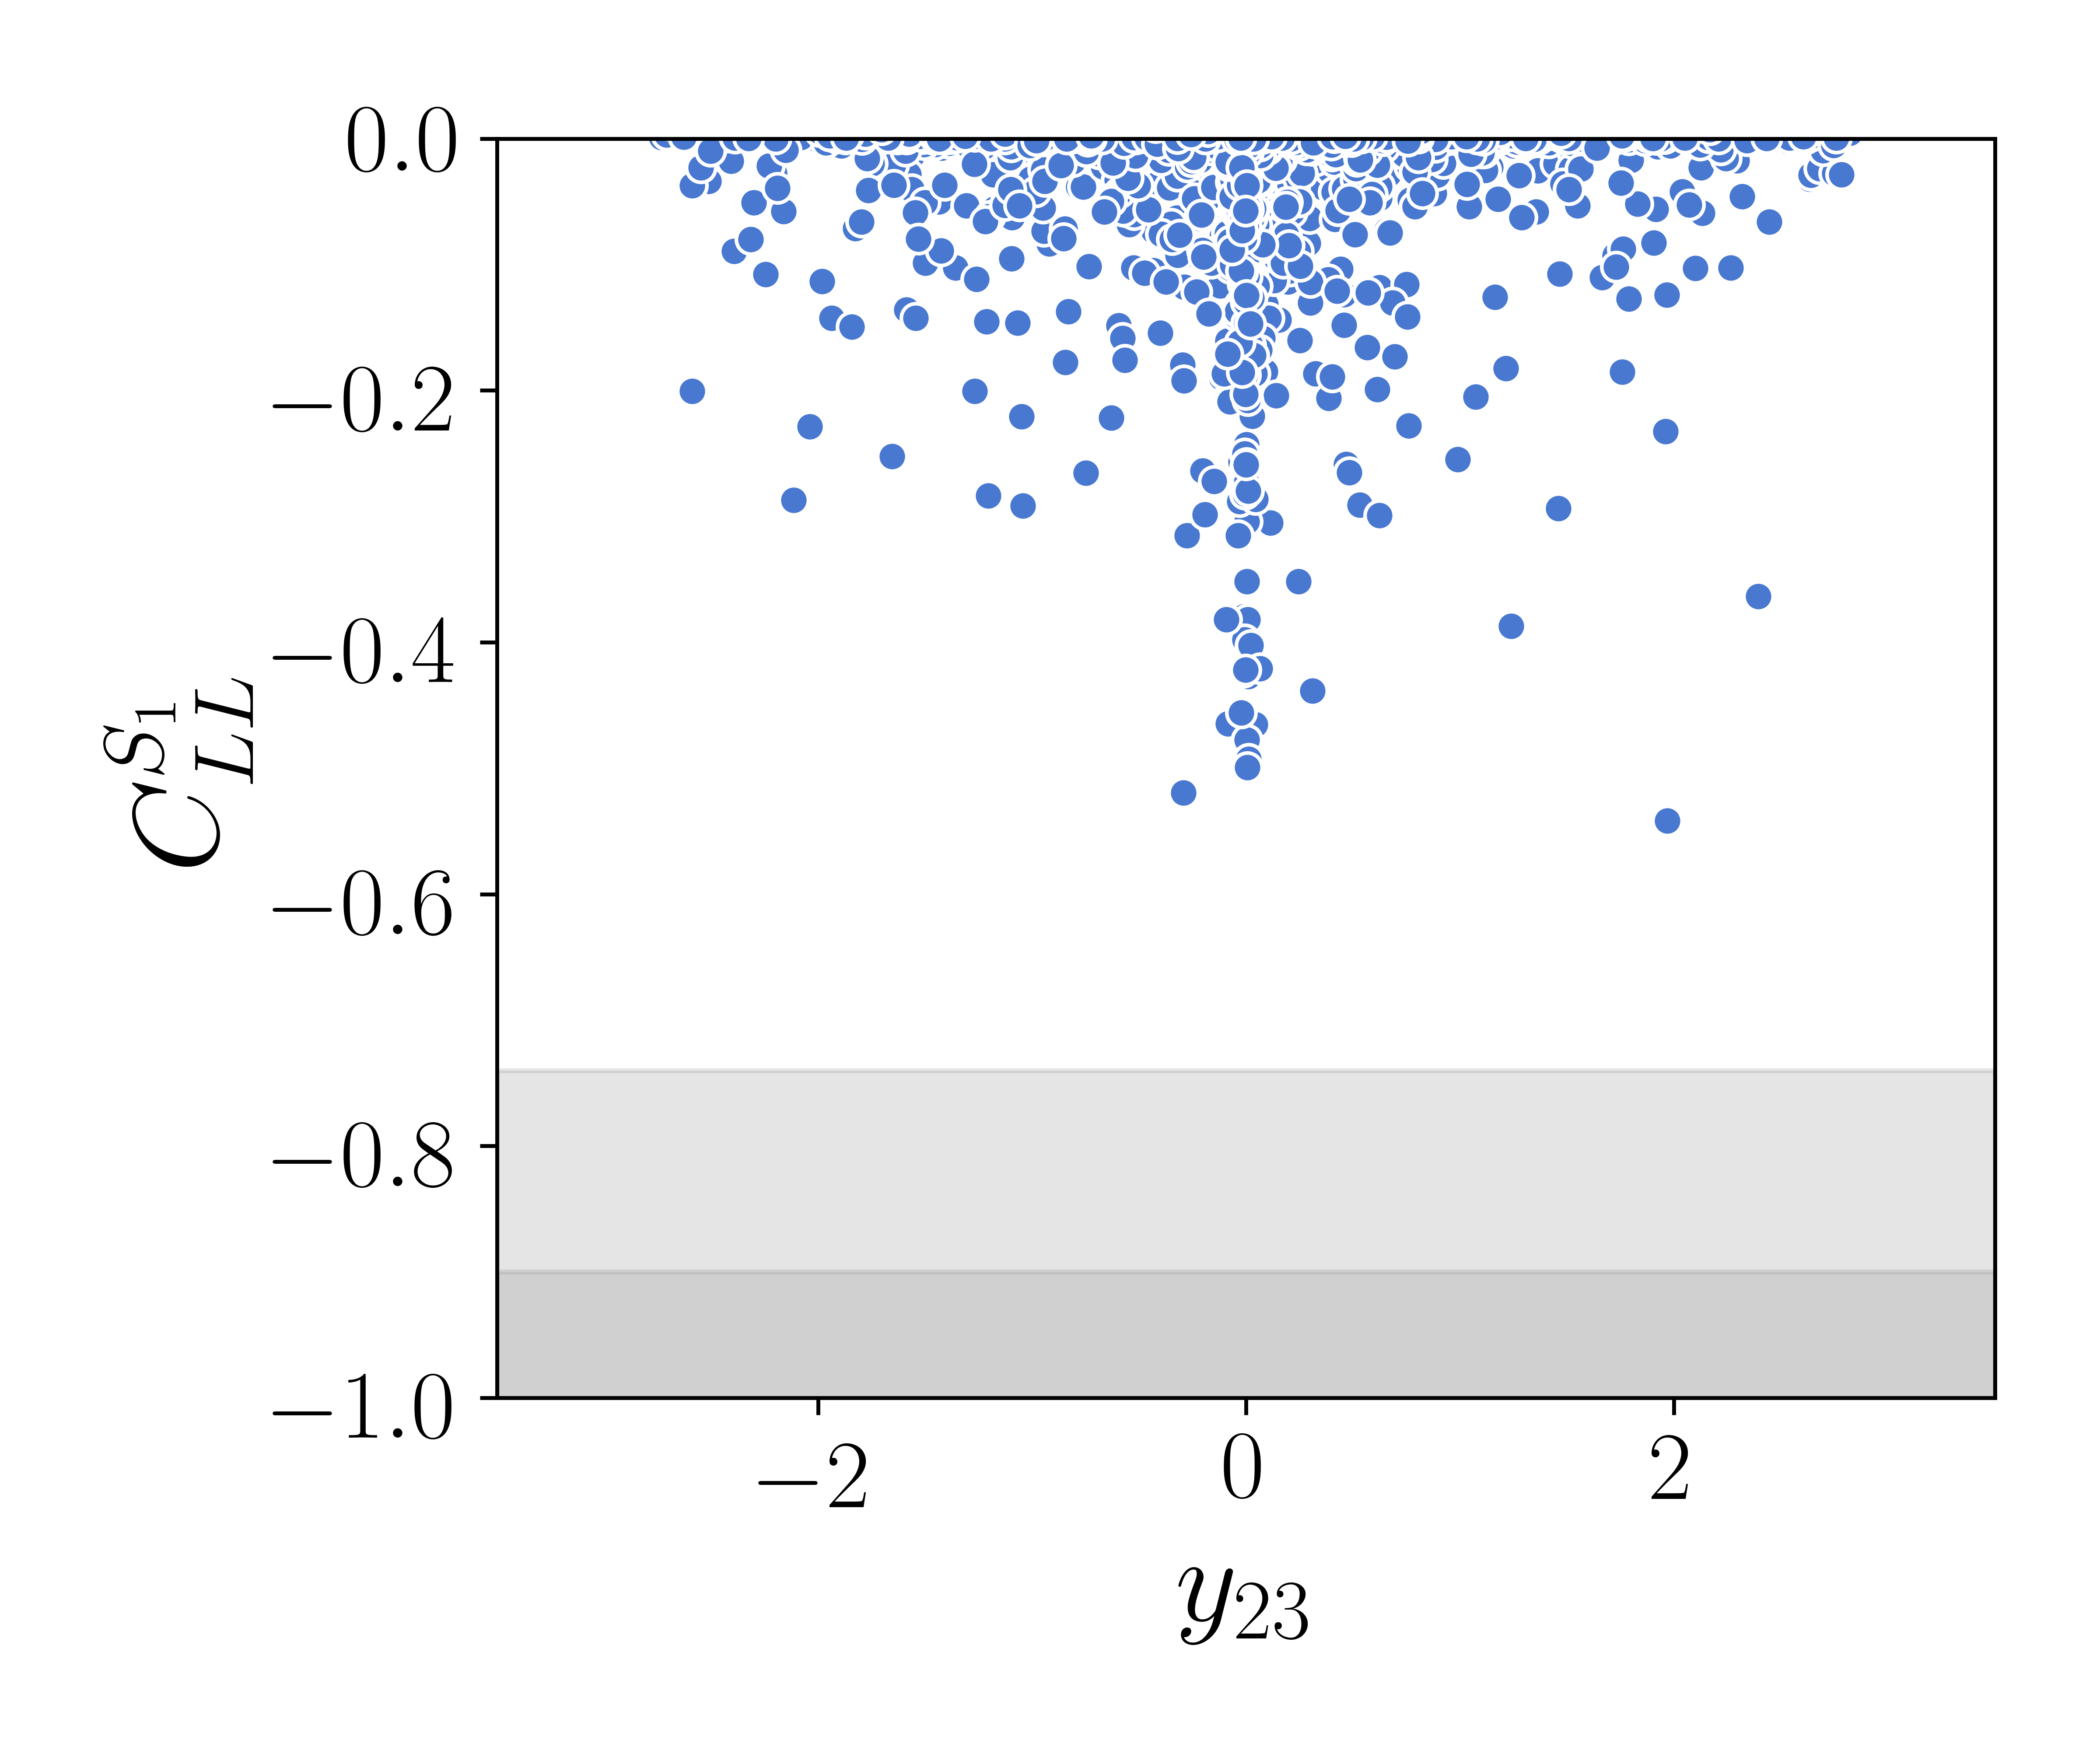
\includegraphics[width=0.40\textwidth]{new_clly23.png}
    \caption[Slices through the parameter space investigated through scan
    II.]{Slices through the parameter space investigated through scan II. The
      value of $C_{LL}^{S_{1}}$ is plotted against each Yukawa coupling scanned
      over. Plots against the $x_{rs}$ contain points from scan II and hence $1$
      and $2\sigma$ regions for $C^{S_{1}}_{LL}$ can be specified since
      $C^{S_{1}}_{LR} = 0$; these are shaded grey. Large values of $x_{23}$ are
      essential for an adequate explanation of the $b \to s$ data in this model,
      while small, but non-zero, values for $x_{22}$ are necessary to allow
      $C_{LL}^{S_{1}}$ to be negative. The values of $x_{23}$ required to
      explain the LFU observables to $2\sigma$ begin to impinge on the
      perturbativity constraint $|x_{23}| < \sqrt{4\pi}$. Only points implying
      SM-like $R_{D^{(*)}}$ are shown.}
  \label{fig:ch3-rkscans}
\end{figure}

\paragraph{Explaining $R_{D^{(*)}}$.} We move on to consider the extent to which
the leptoquark can explain the anomalies in the $b\to c$ transition. The fit
presented in Fig.~\ref{fig:ch3-fit} suggests two scenarios for explaining the
measured tensions in the $b \to c \ell \nu$ decays: (i) new physics only in
$C_V^{33}$; or (ii) new-physics in $C_S^{33}$ and $C_T^{33}$, perhaps along with
contributions in $C_{V}^{33}$. Possibility (i) is the region of parameter space
considered in the model's original form. However, we emphasise that the
conditions presented in Eq.~\eqref{eq:ch3-bnunucond} and
Eq.~\eqref{eq:ch3-eqZll} are sufficient to preclude that effects in $C_V^{33}$
alone could be responsible for the enhancement of the $R_{D^{(*)}}$ ratios. The
product $x_{32}^* x_{33}$ is heavily constrained from $R_K^{\nu\nu}$ and
$B_s$--$\bar{B}_s$ mixing, as indicated in Fig.~\ref{fig:ch3-rknunuallowed}. One
could consider generating $z_{23}$, and therefore $C_V^{33}$, through quark
mixing, thus making do only with a non-zero $x_{33}$ and avoiding these
constraints. This set-up, however, requires excessively large values of $x_{33}$
to explain $R_{D^{(*)}}$, causing the leptoquark's contributions to the
$Z\tau\bar{\tau}$ coupling to exceed current experimental limits---a result we
illustrate in Fig.~\ref{fig:ch3-rDRes}. In addition, we find the effects of
lepton-flavour violation to be subdued, since such contributions add
incoherently to the $W$-mediated SM processes, and thus entail couplings large
enough to conflict with measurements of $B_s$--$\bar{B}_s$ mixing and precision
electroweak observables. Scenario (ii) involves new physics in $C_S^{rs}$ and
$C_T^{rs}$. The most minimal approach here is to turn on only the
bottom--tau-neutrino interaction $x_{33}$ and the right-handed tau--charm
coupling $y_{32}$. A non-zero $x_{33}$ will generate $C_V^{33}$ through
quark-mixing. We find the coupling $y_{32}$ to be weakly constrained by the
precision electroweak measurements discussed earlier: in the limit
$|y_{32}| \gg |y_{3 (1,3)}|$, the bound
\begin{equation}
  |y_{32}| < \frac{3.69 \hat{m}_{S_{1}}}{\sqrt{1 + 0.39 \ln \hat{m}_{S_{1}}}},
\end{equation}
follows from Eq.~\eqref{eq:ch3-eqZll}. In addition, small values of the
muon--top coupling $y_{23}$ will allow sizeable contributions to $(g-2)_\mu$ in
the presence of $x_{23} \neq 0$ because of the top-mass enhancement in the
mixed-chirality term of Eq.~\eqref{eq:ch3-amu}. This minimal texture involving
only third-generation couplings to left-handed quarks comes with the additional
benefit that the leptoquark can evade the constraints from measurements of
$R_{K^{*}}^{\nu\nu}$ and $B_s$--$\bar{B}_s$ mixing. In fact, the only serious
constraint is that arising from the modification of the $Z\tau\bar{\tau}$
coupling from a large $x_{33}$, a situation that can be remedied for
$y_{32} \sim \mathscr{O}(1)$, allowing a good fit to the $R_{D^{(*)}}$ data for
slightly smaller values of $x_{33}$. A sizeable $y_{32}$ is thus a necessary
requirement for this leptoquark model to explain the experimental anomalies in
$R_D$ and $R_{D^*}$. Note also that the measured tension in $(g-2)_\mu$ can be
accommodated at the same time since the couplings involved are unimportant for
$b \to c \tau \nu$. Saturating both $x_{33}$ and $y_{32}$ at the perturbativity
bound $\sqrt{4\pi}$, we find that an explanation of $R_{D^{(*)}}$ loses
viability at $\sim \SI{10}{\TeV}$.

\begin{figure}[t]
  \centering
  \begin{minipage}[t]{0.45\linewidth}
    \centering 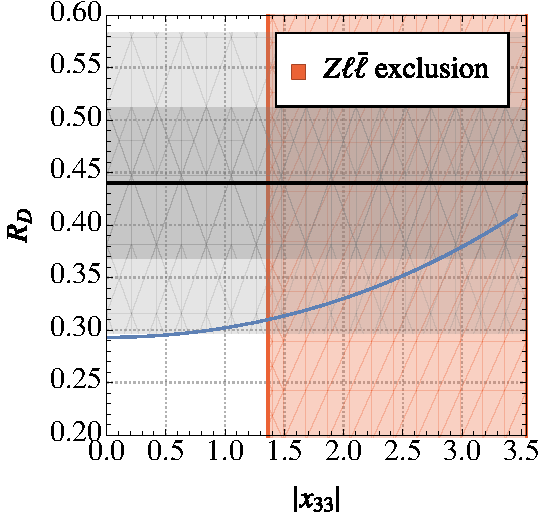
\includegraphics[scale=0.7]{rDRes.pdf}
  \end{minipage}
  \hfill
  \begin{minipage}[t]{0.45\linewidth}
    \centering 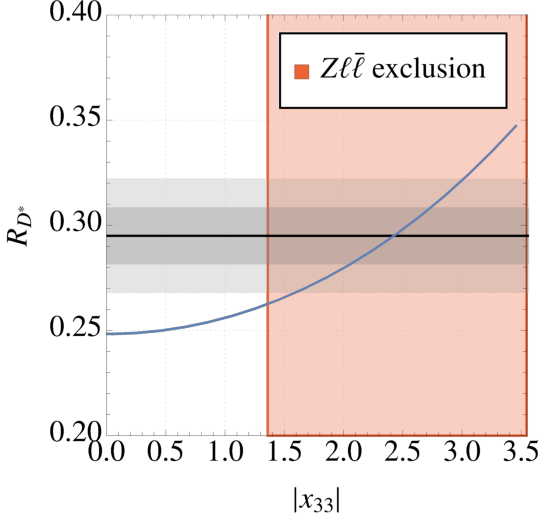
\includegraphics[scale=0.7]{rDStarRes.pdf}
  \end{minipage}
  \caption[The solid blue lines represents the dependence of $R_D$ (left) and
  $R_{D^{(*)}}$ (right) on $|x_{33}|$ when all other couplings are set to zero
  and $m_{S_{1}} = \SI{1}{\TeV}$.]{The solid blue lines represents the dependence
    of $R_D$ (left) and $R_{D^{(*)}}$ (right) on $|x_{33}|$ when all other
    couplings are set to zero and $m_{S_{1}} = \SI{1}{\TeV}$. A non-zero $x_{33}$
    generates a small $z_{32}$ through the quark mixing of
    Eq.~\eqref{eq:ch3-mixing}, although the $|x_{33}|$ values required to meet the
    anomalies become large enough to dangerously modify the $Z \to \tau\tau$
    rate. The values of $|x_{33}|$ excluded by measurements of the $Z\tau\tau$
    coupling are shaded red. The solid black line represents the central values
    of the measurements for $R_D$ and $R_{D^{(*)}}$, and the grey areas are the
    $1$ and $2\sigma$ regions.}
  \label{fig:ch3-rDRes}
\end{figure}

In Fig.~\ref{fig:ch3-money1} we present the results of scan II in the
$R_D$--$R_{D^*}$ plane, while Fig.~\ref{fig:ch3-ObsScans} displays the values of
the Yukawa couplings from the same scan that lead to interesting $R_{D^{*}}$ values.
Limits on the $B \to K^{*} \nu \nu$ rate and measurements of $B_s$--$\bar{B}_s$
mixing constrain the $x_{r2}$ to be small, while large values for $x_{33}$ and
$y_{32}$ are necessary since their product appears in the expressions for
$C_{ V }^{33}$, $C_{ S }^{33}$ and $C_{ T }^{33}$. As discussed above, these
large $x_{33}$ values imply dangerous contributions to $Z \to \tau \tau$,
causing few points to stray into the $1\sigma$ region. The model can, however,
significantly reduce the tension in the $b\to c \tau \nu$ measurements in a
large region of parameter space.

\begin{figure}[t]
  \centering 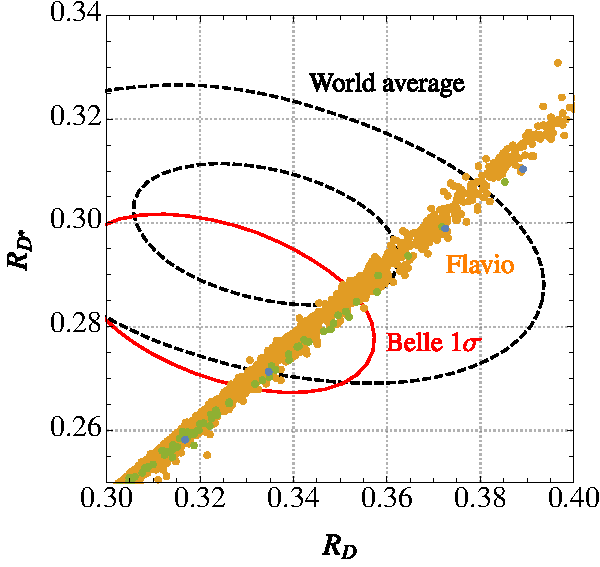
\includegraphics[width=0.6\linewidth]{rdrdstarNew.pdf}
  \caption[The results of scan II presented as a scatter plot of $R_D$ against
  $R_{D^*}$.]{The results of scan II (orange points) presented as a scatter plot
    of $R_D$ against $R_{D^*}$. The dashed black ellipses represent the $1$, $2$
    and $3\sigma$ contours from our fit with an assumed correlation
    $\rho = -0.2$, while the solid red curve indicates the $1\sigma$ allowed
    region implied by the Belle measurement from Ref.~\cite{Abdesselam:2019dgh}.
    The green points place $C_{LL}$ in the $3\sigma$ region of the fit of
    Ref.~\cite{Aebischer:2019mlg}, while the blue points place $C_{LL}$ within
    the $2\sigma$ region. It is clear that the anomalies in $b \to c \tau \nu$
    can be well accommodated in this model, with relatively good agreement with
    the $b \to s$ data at the same time. Almost all of the points in the region
    of interest contribute along the scalar--tensor direction.}
  \label{fig:ch3-money1}
\end{figure}

\begin{figure}
    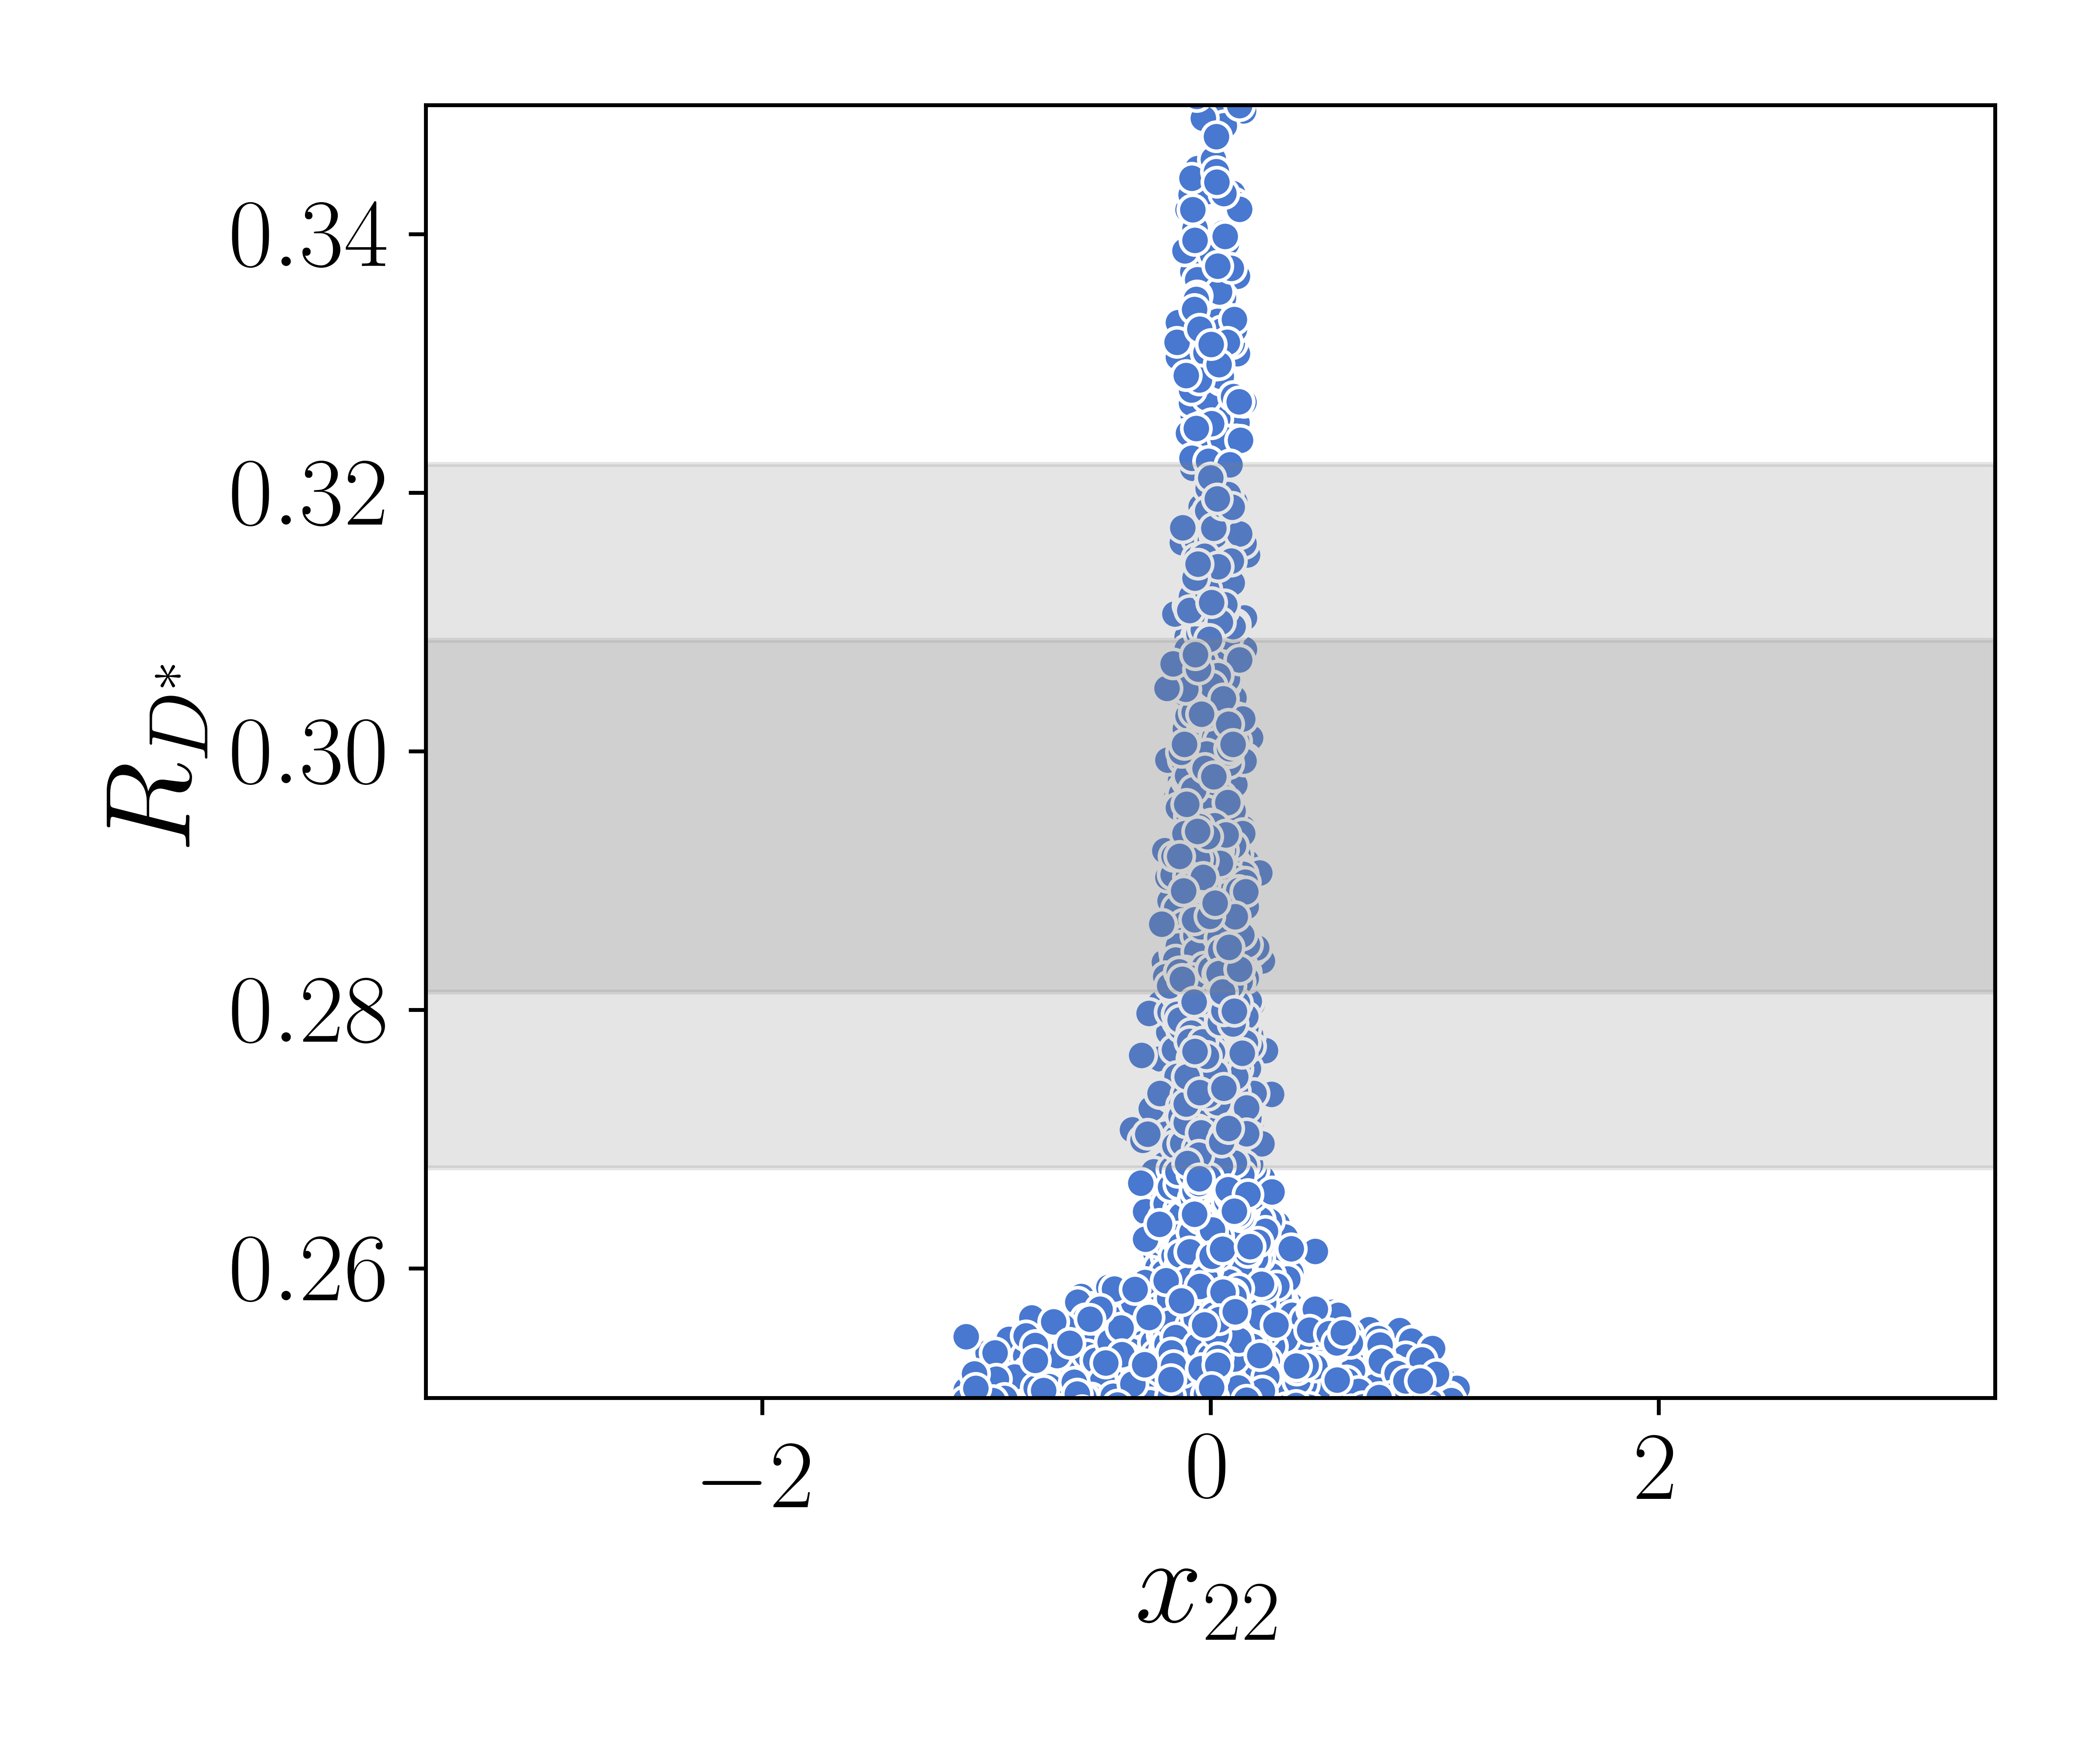
\includegraphics[width=0.49\textwidth]{new_obsx22.png} \hfill
    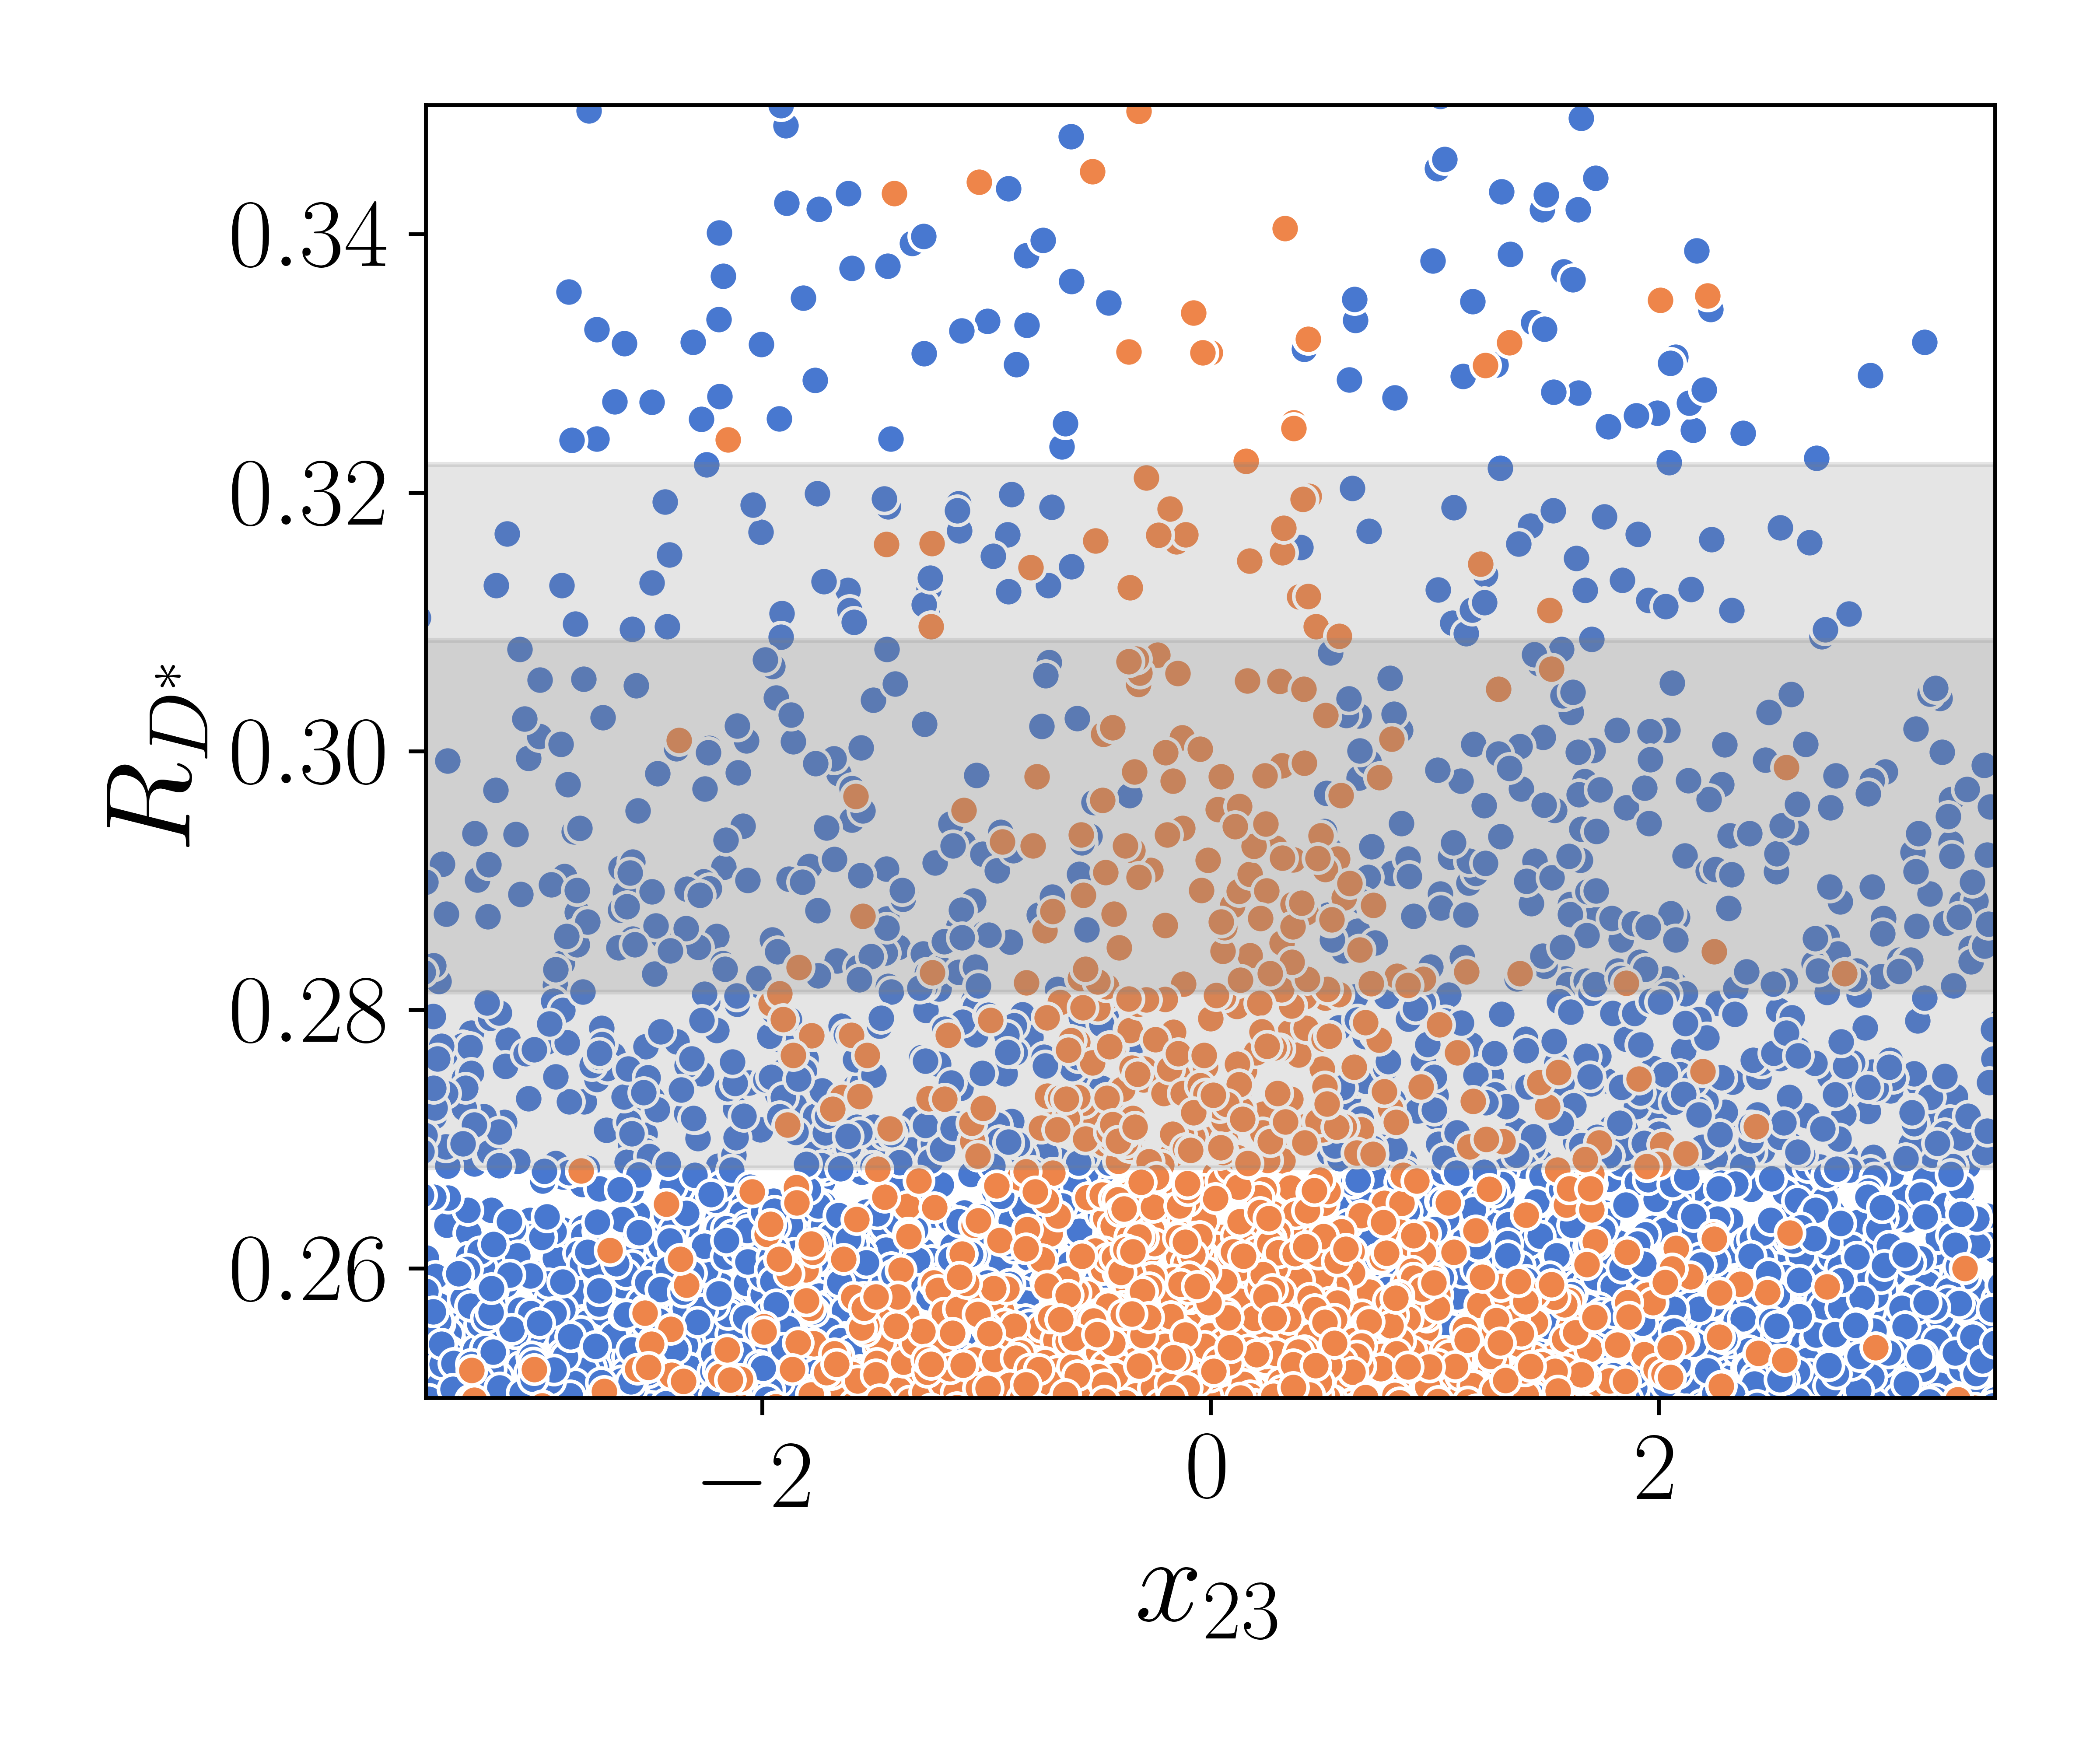
\includegraphics[width=0.49\textwidth]{new_obsx23.png} \\
    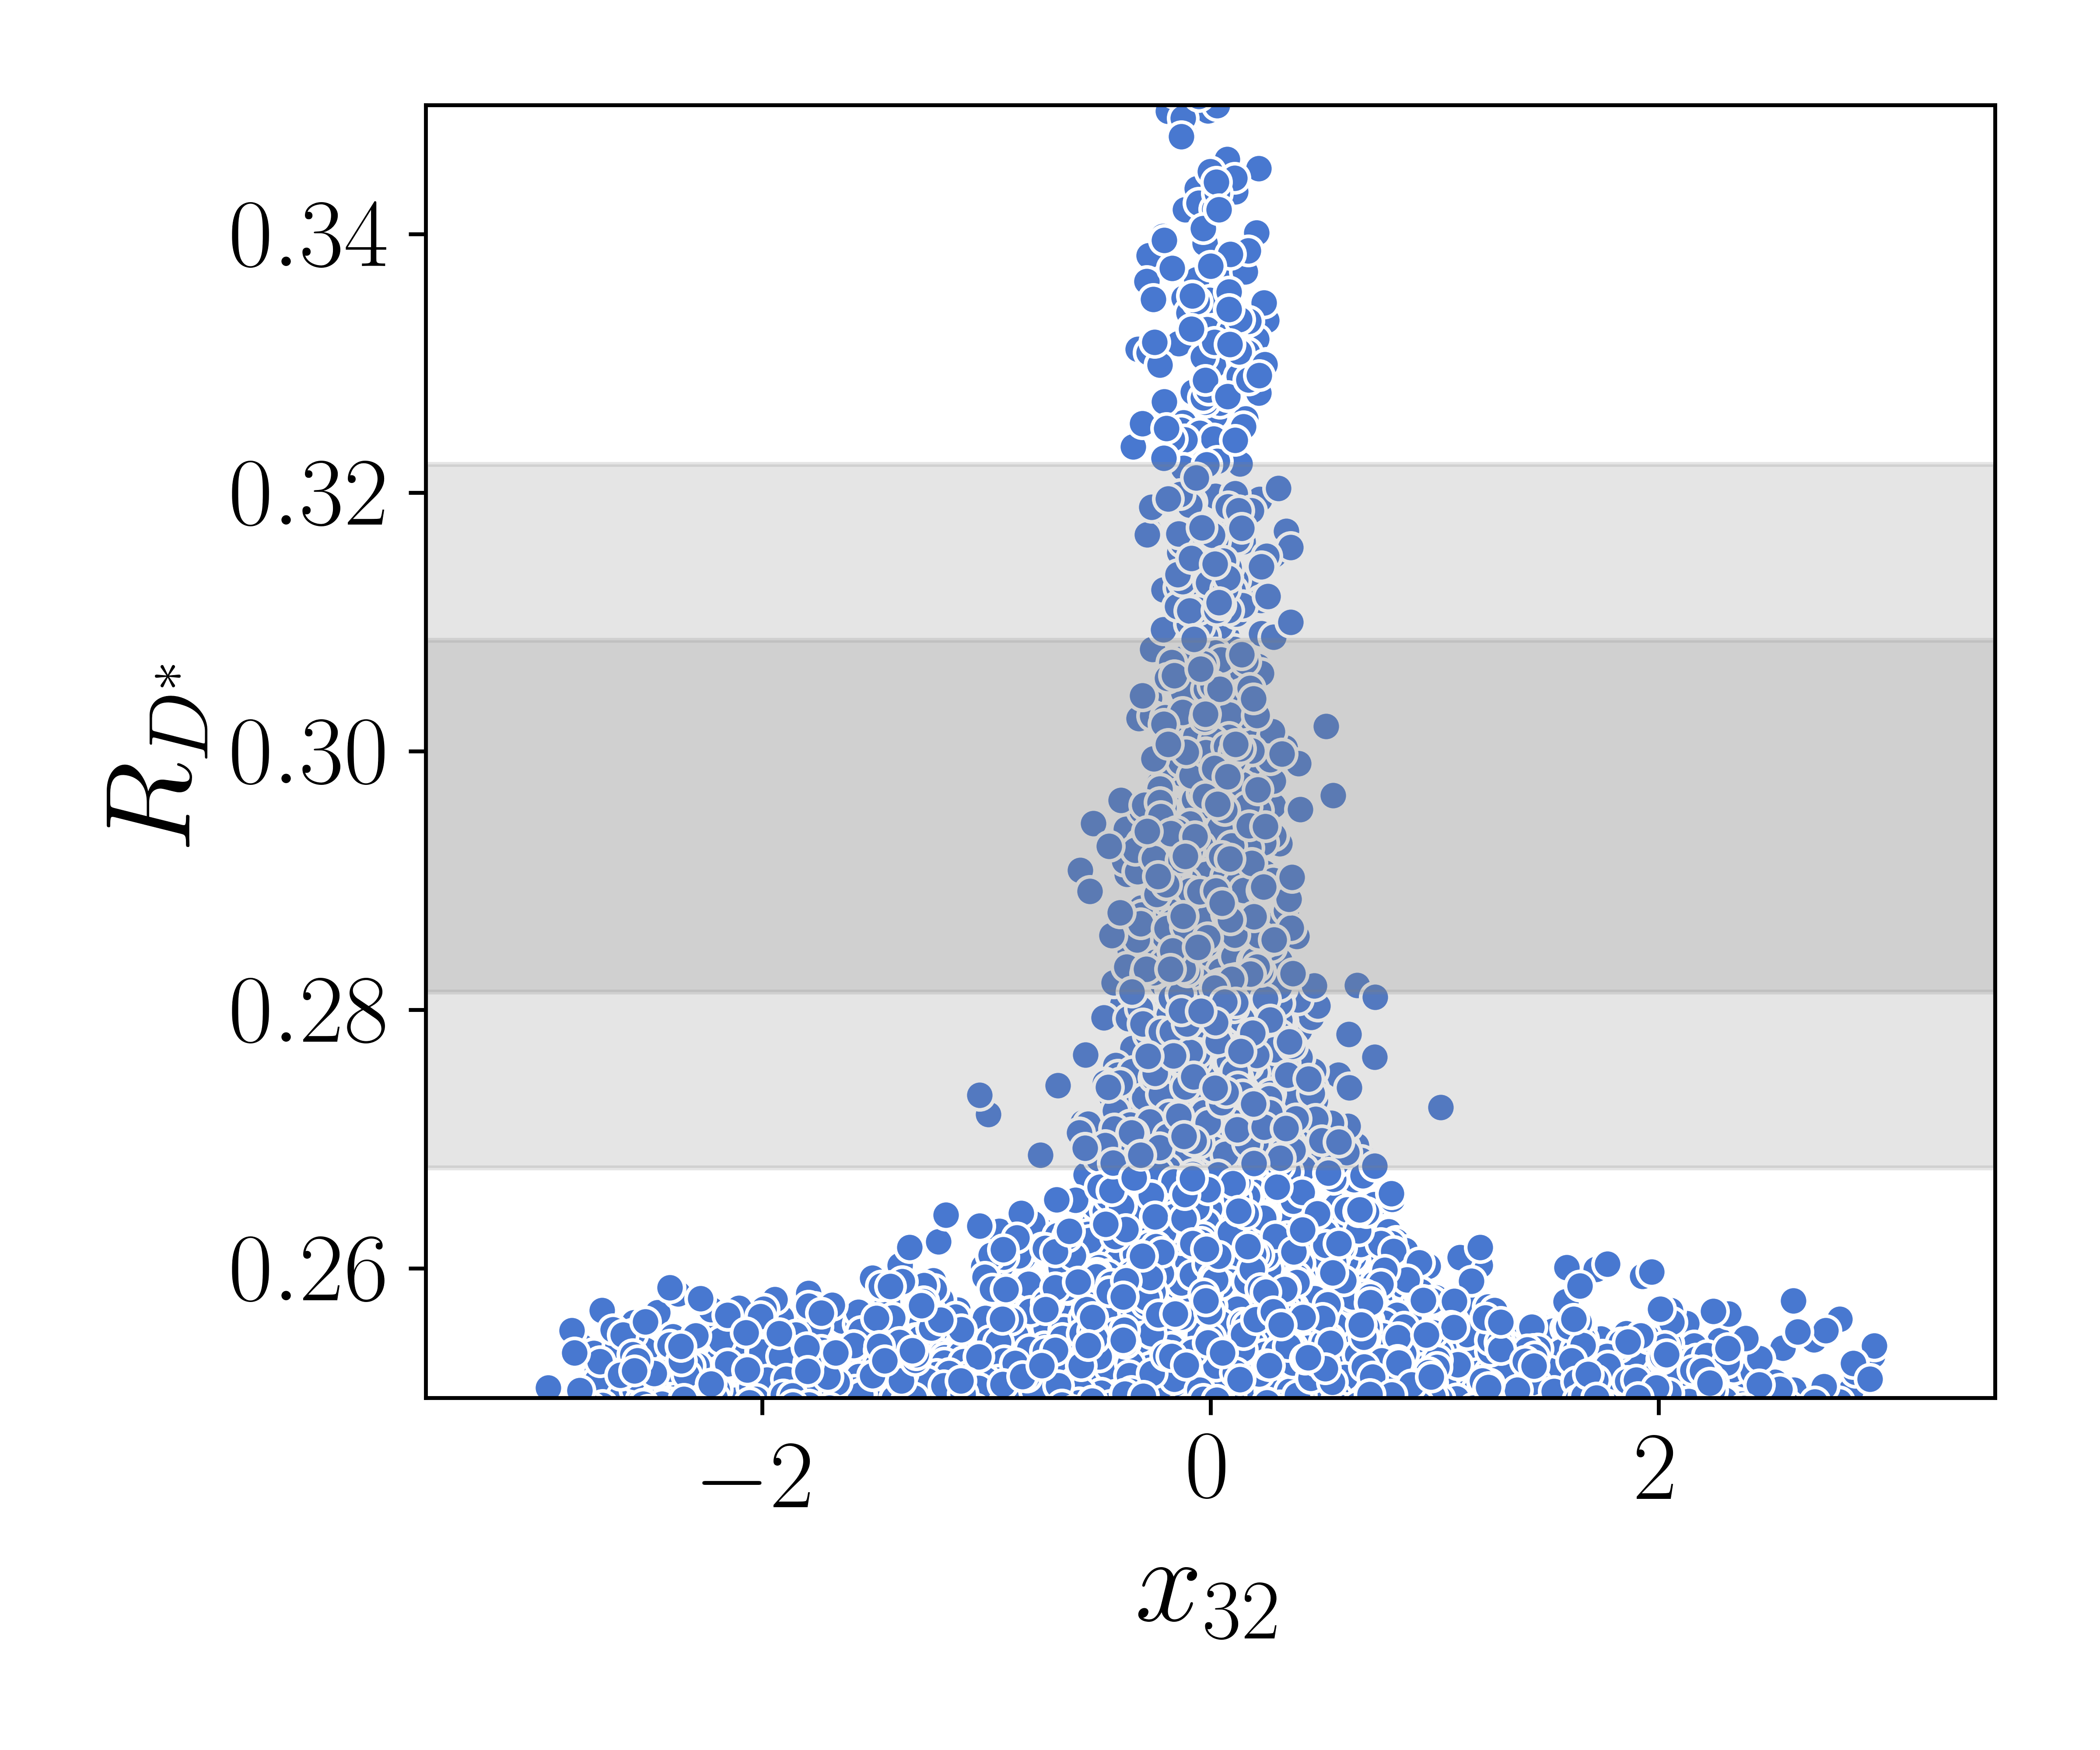
\includegraphics[width=0.49\textwidth]{new_obsx32.png} \hfill
    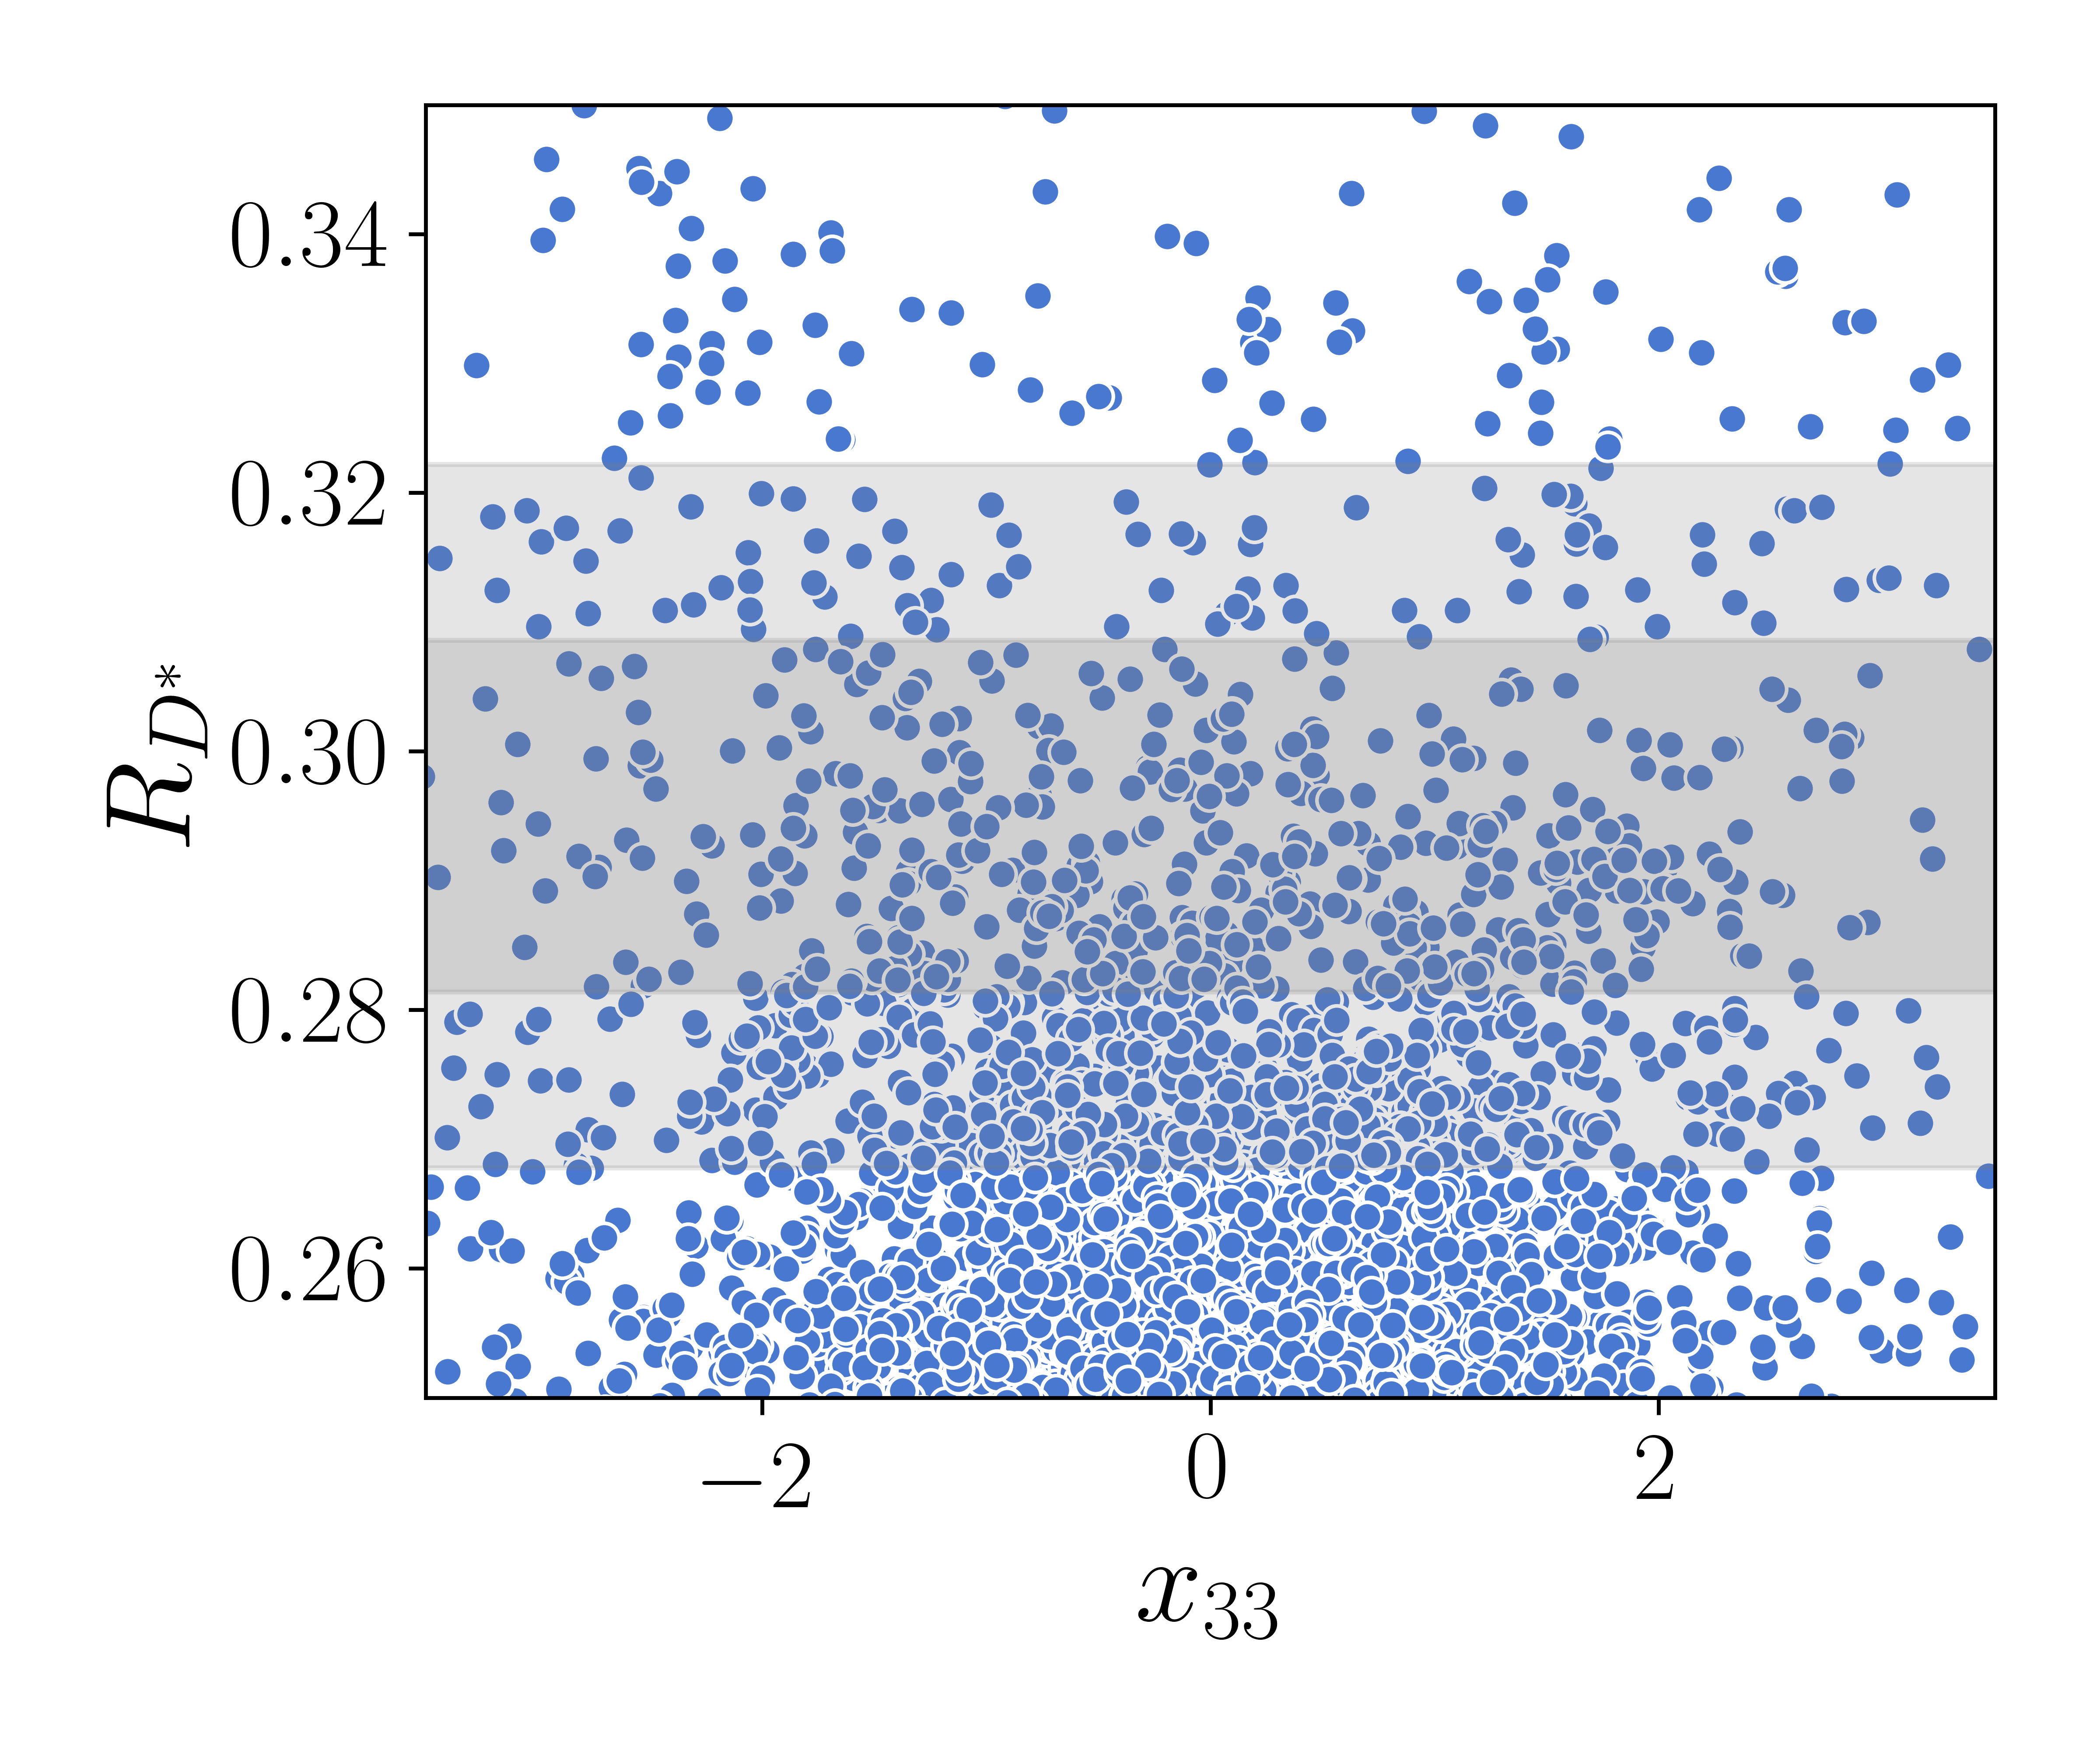
\includegraphics[width=0.49\textwidth]{new_obsx33.png} \\
    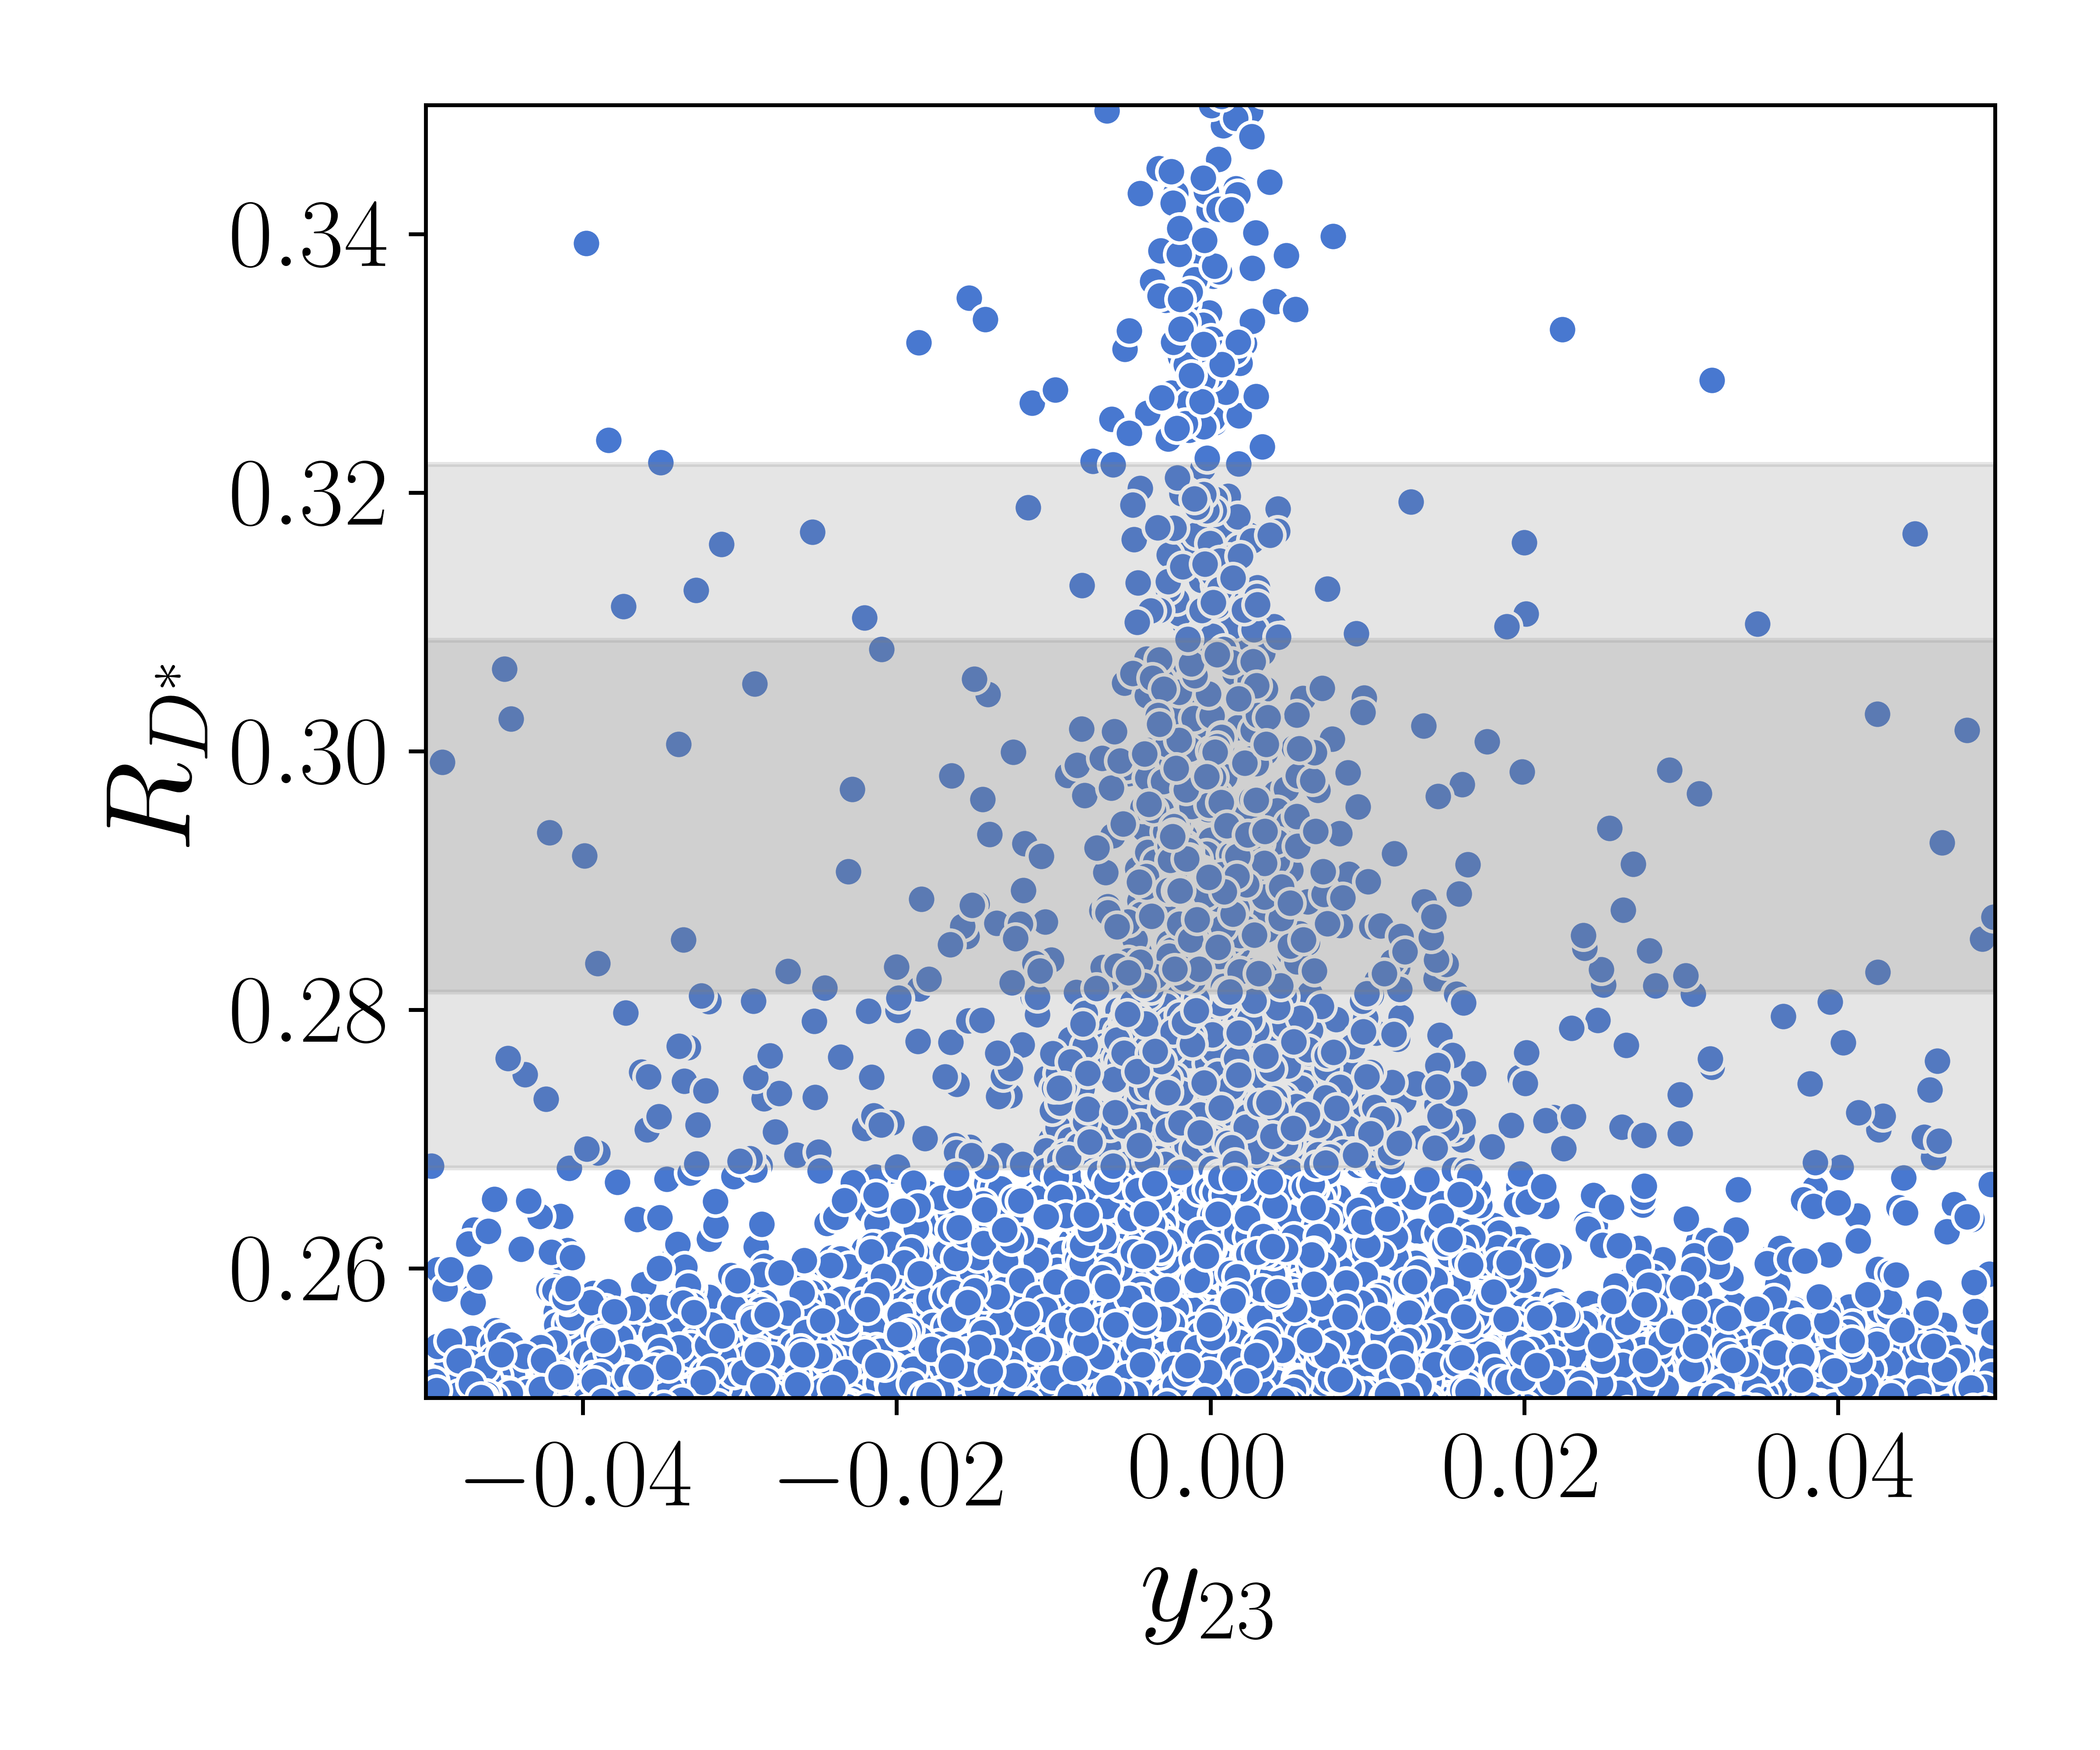
\includegraphics[width=0.49\textwidth]{new_obsy23.png} \hfill
    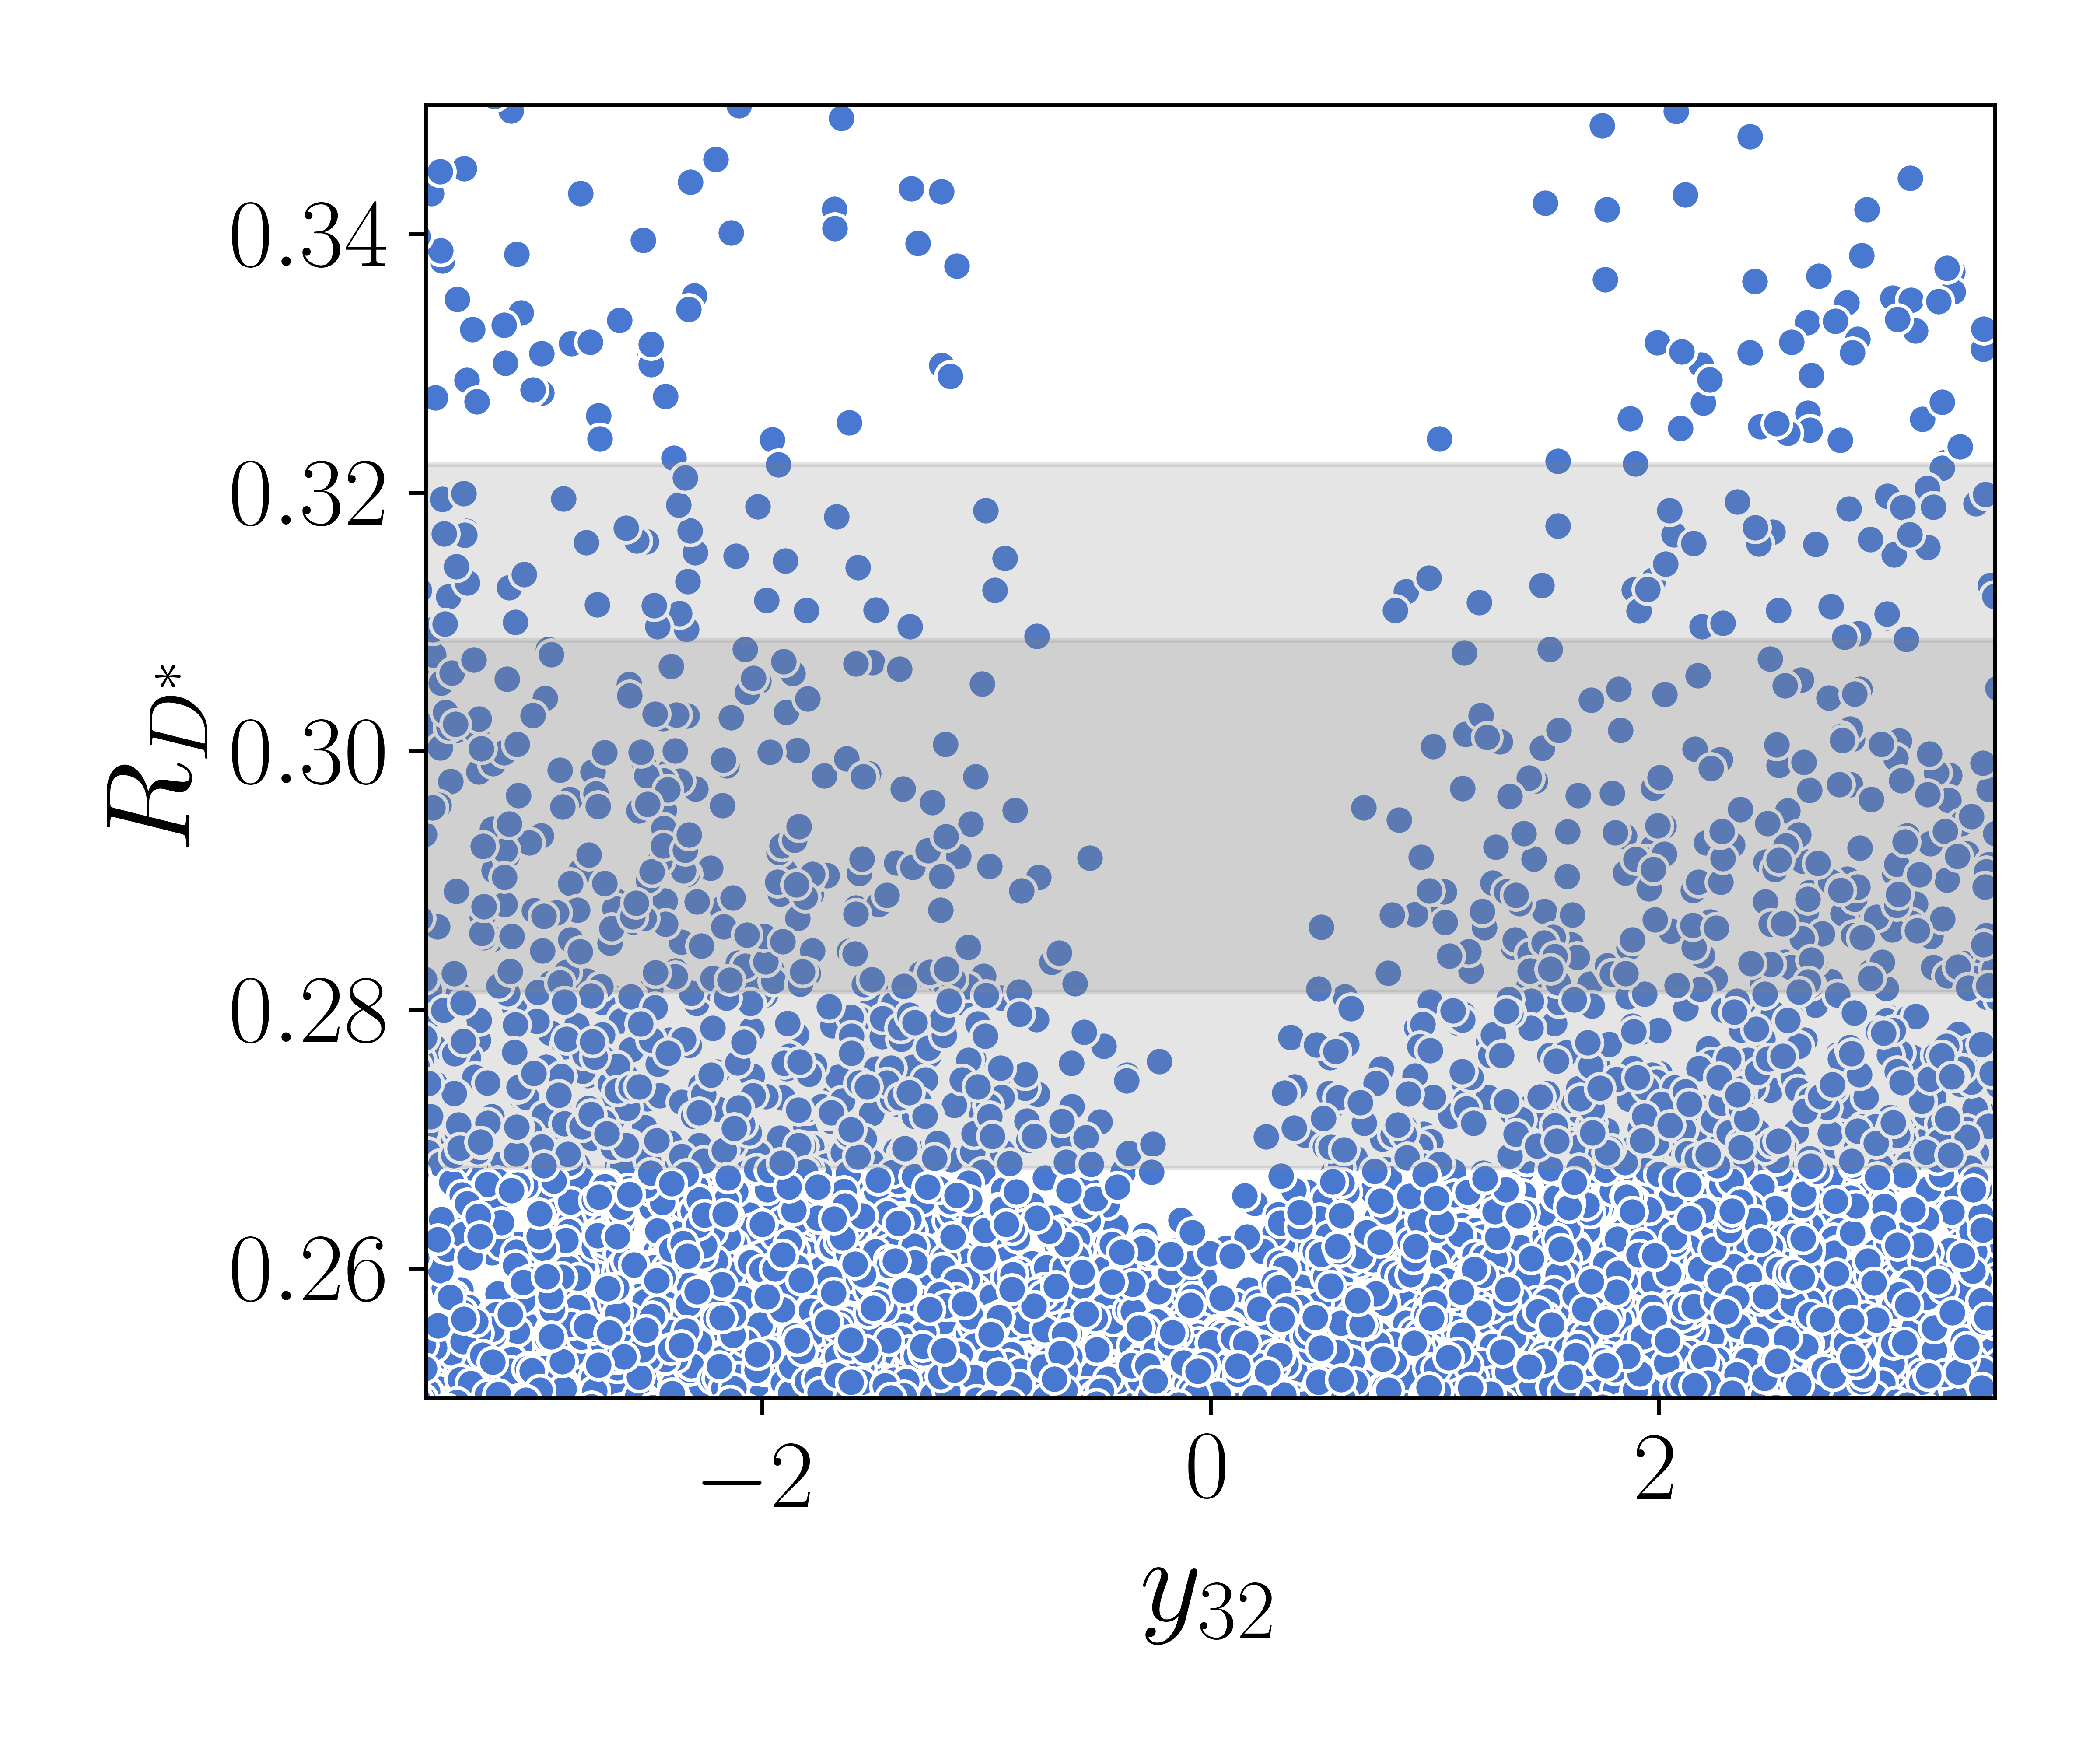
\includegraphics[width=0.49\textwidth]{new_obsy32.png}
    \caption[Slices through the parameter space of scan II shown against
    $R_{D^{*}}$.]{Slices through the parameter space of scan II shown against
      $R_{D^{*}}$. The grey bands correspond to the $1$ and $2\sigma$ regions
      for the measurements to $R_{D^{*}}$. The orange points keep $C_{LL}$
      SM-like, while blue points show $> 1\%$ deviation in $C_{LL}$ from the SM
      prediction. Large values $x_{33}$ and $y_{32}$ are necessary for an
      adequate explanation of $R_{D^{*}}$ since these feature in $C_S$ and $C_T$.
      Other left-handed couplings must be small to evade constraints from
      $R_K^{\nu\nu}$ and $B_s$--$\bar{B}_s$ mixing. The results for $R_{D}$ are
      qualitatively the same.}
  \label{fig:ch3-ObsScans}
\end{figure}

\paragraph{Other $b \to c$ observables.} The fit we present in
Sec.~\ref{sec:ch3-signals} does not include the less-precisely measured
observables $R_{J/\psi}$, $f_L^{D^*}$ and $\mathcal{P}_\tau^*$, introduced in
section.~\ref{sec:ch1-chargedcurrentanomalies}. We instead use the preferred
values from our fit to make predictions for these observables, concentrating on
the scalar--tensor solution, since we find this to be the easiest to accommodate
with the leptoquark. We note that this solution gives negligible efficiency
variation from the SM for the measurement in the $D^*$ mode~\cite{Sato:2016svk}
and displays a $q^2$ spectrum that agrees well with
experiment~\cite{Freytsis:2015qca}.

In figure~\ref{fig:ch3-btocpredictions} we project the $2\sigma$ preferred
region for $C_{S_L}$ (see Table~\ref{tab:ch3-fitresults}) onto combinations of
$b \to c$ related observables to illustrate the ability of combined measurements
to close in on this scenario. Were possible, we have also shown Belle II
$50 \text{ ab}^{-1}$ sensitivity~\cite{Alonso:2017ktd} in grey centred around
the SM prediction in black. Current measurements are shown in red with their
$1 \sigma$ errors in orange. With contributions in the scalar--tensor direction,
the $S_{1}$ leptoquark's contributions to $f_L^{D^*}$ are in the opposite
direction to current measurements, although still within the $2\sigma$ region.
If the central value of $f_L^{D^*}$ stays close to where it is, or moves down
slightly, the model would then predict $\mathcal{P}_\tau \approx 0.4$, which
compromises the potential mild improvement in $R_{J/\psi}$ the model can offer.
This scenario leads to a SM-like $\mathcal{P}_{\tau}^*$, but potentially large
deviations in the $\mathcal{P}_{\perp}^{(*)}$ observables.

\begin{figure}[t]
  \centering
  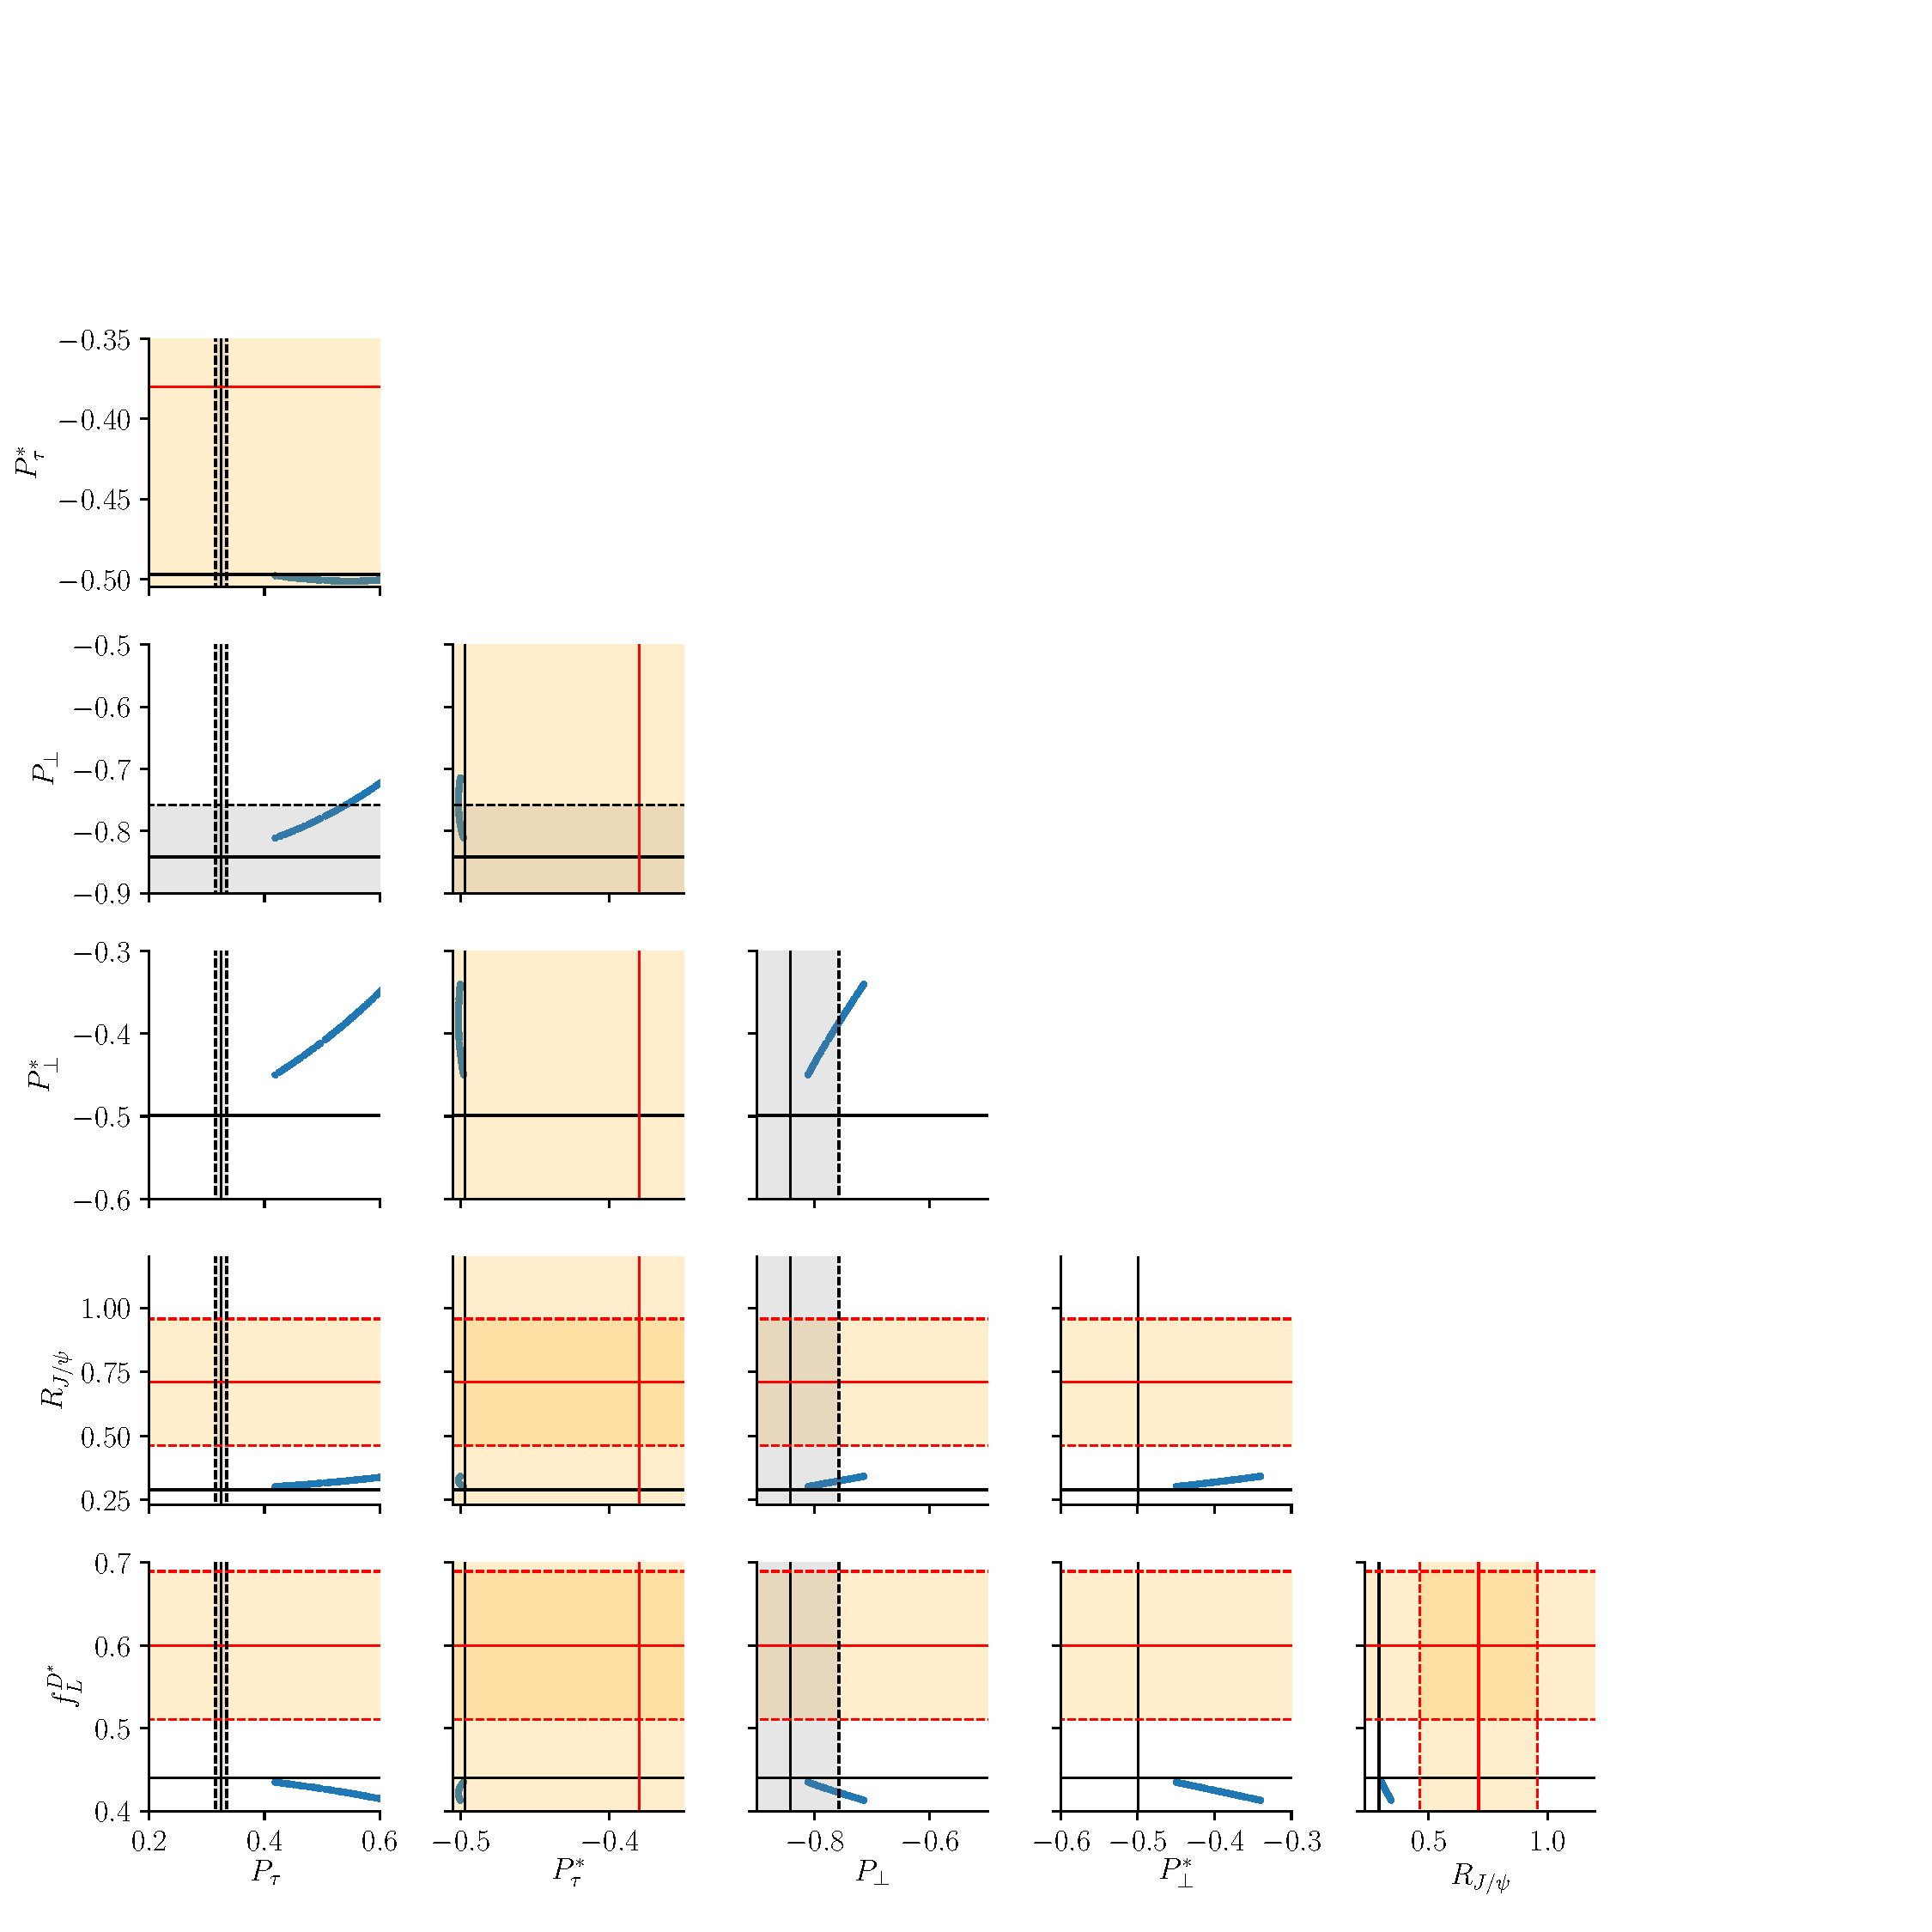
\includegraphics[width=\textwidth]{pairplot}
  \caption[A grid plot of the various $b \to c$ related observables in addition
  to $R_{D}$ and $R_{D^*}$ considered in our analysis.]{A grid plot of the
    various $b \to c$ related observables in addition to $R_{D}$ and $R_{D^*}$
    considered in our analysis. Solid black lines represent the SM predictions
    around which the grey shaded regions are the Belle II $50 \text{ ab}^{-1}$
    sensitivities~\cite{Alonso:2017ktd}, bordered by the black dashed lines. Red
    lines are current measurements and orange regions are their $1\sigma$
    errors. Where the Belle II sensitivity is unavailable we present only the SM
    prediction without a shaded region. The blue points explain $R_{D^{(*)}}$ to
    $2 \sigma$.}
  \label{fig:ch3-btocpredictions}
\end{figure}


\paragraph{Explaining both the $b \to s$ data and $R_{D^{(*)}}$.} In order to
establish the full power of the model to explain both $R_{D^{(*)}}$ and the
$B \to s$ data, we perform a complete scan over the 7-dimensional parameter
space spanned by the leptoquark mass and the couplings $x_{rs}$ for
$r,s \neq 1$, $y_{23}$ and $y_{32}$---the parameters of scan II. Results from
this scan have been presented above in Fig.~\ref{fig:ch3-money1}, where the
green and blue points project the results of scan II into
$C_{LL}$--$R_D$--$R_{D^*}$ space, where colour is used as the third axis. The
green points imply $C_{LL} \in [-1.54, -0.58]$ (the $3\sigma$ region), while the
blue points have $C_{LL} \in [-1.38, -0.74]$ (the $2\sigma$
region)~\cite{Aebischer:2019mlg}. This plot demonstrates a mild tension between
$b \to s$ and $R_{D^{(*)}}$ in this leptoquark model: points lying within the
$1\sigma$ region for $C_{LL}$ keep $R_{D^{(*)}}$ SM-like. This can be attributed
to the behaviour evident in Fig.~\ref{fig:ch3-x33x32rat}: large, negative values
of $C_{LL}^{S_{1}}$ require $x_{33} \approx 0$, but $x_{33}$ is essential to
this model's explanation of $R_{D^{(*)}}$, since it features in
$C^{33}_{V,S,T}$. At best, we find that the model can explain all of the
discrepant measurements to within $2\sigma$, a striking level of consistency
with all constraints and anomalies. In both cases the $(g-2)_\mu$ anomaly can
also be accommodated.

\section{Conclusions}

We have reconsidered the potential of a scalar leptoquark
$S_{1} \sim (\mathbf{3},\mathbf{1},-1/3)$ to explain recent $B$-physics
anomalies: the LFU ratios $R_{K^{(*)}}$ and $R_{D^{(*)}}$, anomalies in
branching ratio data and angular observables in the $b \to s$ transition, as
well as the anomalous magnetic moment of the muon.

The leptoquark can reduce the tension in the $R_{D^{(*)}}$ observables to within
$1\sigma$ of their current experimental values at the price of a sizeable
coupling to the right-handed tau and charm quark. The explanation loses
viability for masses above about \SI{10}{\TeV}. The leptoquark can also reduce
the tensions in the $b \to s$ data, albeit at some expense to the explanation of
$R_{D^{(*)}}$. Explicitly, the region of parameter space in which $R_{D^{(*)}}$
is accommodated to within $1\sigma$ implies $C_{LL}$ values differing from the
SM value by $< 1\%$, and coupling textures explaining the neutral-current
anomalies to within $1\sigma$ keep $R_{D^{(*)}}$ within theoretical uncertainty
from SM prediction. At best, we find that the model can accommodate the combined
tensions in both the $b \to s$ and $b \to c$ transitions to within $2\sigma$ as
well as eliminate the tension in $(g-2)_\mu$, a remarkable feat for a
single-particle extension of the SM.

A crucial new ingredient for this model's explanation of $R_{D^{(*)}}$ is the
consideration of the area of parameter space in which the coupling $y_{32}$ is
large. The combination of right- and left-handed couplings induces scalar and
tensor operators, which lift the chirality suppression of the $B$-meson decays
and consequently produce a sizeable new-physics contribution. Moreover the
tensor contribution resolves a possible tension induced by the scalar
contribution to leptonic charmed $B$-meson decays, $B_c\to\tau\nu$. In our
numerical scans we found that the right-handed Yukawa coupling $y_{32}$ need
take $\mathscr{O}(1)$ values, while the left-handed couplings $x_{22}$ and
$x_{32}$ and the right-handed coupling $y_{22}$ are required to be small.
Interestingly, this model predicts a value of $R_{D^*}$ slightly smaller than
that suggested by current data, consistent with the Belle results. Future
measurements of the asymmetry observable $P_\tau$ by Belle II can also test this
model, which prefers $P_\tau \approx 0.4$, assuming the central values of
$f_L^{D^*}$ and $R_{D^{(*)}}$ remain constant.

An explanation of $b \to s$ data requires $\mathscr{O}(1)$ couplings of the
leptoquark to the muon, a scenario in conflict with the experimental
measurements of the decays of the $Z$ boson and $D^0$ mesons in the context of
this leptoquark model. Moreover, the tension between the preferred value of
$C_{LL}$ and the lepton universality ratio $R_{D^{(*)}}^{\mu/e}$, pointed out in
Ref.~\cite{Becirevic:2016oho}, is naturally relieved for leptoquark masses
$m_{S_{1}} \gtrsim \SI{1}{\TeV}$. Consequently, the best fit to the $b \to s$
data (requiring large, negative values of $C_{LL}^{S_{1}}$) is obtained for
large leptoquark masses of $\sim \SI{5}{\TeV}$ with a large hierarchy between
the left-handed couplings $|x_{32}|\gg|x_{33}|$ to avoid constraints from
$\tau\to \mu$ LFV transitions.

Apart from the anomalies in lepton flavor universality ratios, the leptoquark
can easily account for the anomalous magnetic moment of the muon by an
appropriate choice of the product of couplings $y_{23} z_{23}$.

At a future $100 \text{ TeV}$ proton--proton collider the pair-production cross
section of the leptoquark will be substantially enhanced compared to the LHC
with about \SI{1}{\fb} for a \SI{5}{\TeV} leptoquark~\cite{Arkani-Hamed:2015vfh}
and thus will be able to probe most of the relevant parameter space for the
$B$-physics anomalies studied here.
